%! TEX program = pdflatex
\documentclass[aspectratio=169,10pt,xcolor=table]{beamer}

% =========================================================================
% PAQUETES Y CODIFICACIÓN
% =========================================================================
\usepackage[utf8]{inputenc}
\usepackage[T1]{fontenc}
\usepackage[spanish,es-nodecimaldot,es-noshorthands]{babel}
\usepackage{lmodern}
\usepackage{amsmath,amssymb,mathtools,bm}
\usepackage{graphicx}
\usepackage{booktabs}
\usepackage{array}
\usepackage{multirow}
\usepackage{tabularx}
\usepackage{tikz}
\usetikzlibrary{shapes.geometric, arrows.meta, positioning, calc, fit}
\usepackage{hyperref}

% =========================================================================
% PALETA DE COLORES INSTITUCIONAL IPN - ESCOM
% =========================================================================
\definecolor{ipnDark}{HTML}{6B1D2F}
\definecolor{ipnDarker}{HTML}{4E1422}
\definecolor{ipnMed}{HTML}{8A2432}
\definecolor{ipnSoft}{HTML}{F6EEF0}
\definecolor{ipnAccent}{HTML}{D9B8C0}
\definecolor{bgLight}{HTML}{F8F9FA}
\definecolor{textDark}{HTML}{212529}
\definecolor{textMuted}{HTML}{5A626A}
\definecolor{rowLight}{HTML}{F4ECEE}
\definecolor{rowHighlight}{HTML}{EAD6DA}
\definecolor{accentBlue}{HTML}{1B4F72}
\definecolor{accentGreen}{HTML}{1E6B47}
\definecolor{borderGray}{HTML}{D0D5DD}

% =========================================================================
% TEMA VISUAL Y MÁRGENES AMPLIOS (16:9)
% =========================================================================
\usetheme{default}
\usecolortheme{default}
\usefonttheme{professionalfonts}

\setbeamersize{text margin left=10mm, text margin right=10mm}
\setbeamertemplate{navigation symbols}{}

\setbeamercolor{background canvas}{bg=white}
\setbeamercolor{normal text}{fg=textDark,bg=white}
\setbeamercolor{structure}{fg=ipnDark}
\setbeamercolor{palette primary}{bg=ipnDark,fg=white}
\setbeamercolor{palette secondary}{bg=ipnMed,fg=white}
\setbeamercolor{palette tertiary}{bg=ipnDarker,fg=white}
\setbeamercolor{frametitle}{bg=ipnDark,fg=white}
\setbeamercolor{framesubtitle}{fg=ipnAccent}
\setbeamercolor{block title}{bg=ipnDark,fg=white}
\setbeamercolor{block body}{bg=bgLight,fg=textDark}
\setbeamercolor{block title alerted}{bg=ipnMed,fg=white}
\setbeamercolor{block body alerted}{bg=ipnSoft,fg=textDark}
\setbeamercolor{block title example}{bg=accentBlue,fg=white}
\setbeamercolor{block body example}{bg=bgLight,fg=textDark}
\setbeamercolor{itemize item}{fg=ipnDark}
\setbeamercolor{itemize subitem}{fg=ipnMed}
\setbeamercolor{enumerate item}{fg=ipnDark}

\setbeamerfont{frametitle}{size=\normalsize,series=\bfseries}
\setbeamerfont{framesubtitle}{size=\scriptsize,series=\mdseries}
\setbeamerfont{block title}{size=\footnotesize,series=\bfseries}
\setbeamerfont{itemize/enumerate body}{size=\footnotesize}
\setbeamerfont{itemize/enumerate subbody}{size=\scriptsize}

\setbeamertemplate{itemize items}[circle]
\setbeamertemplate{enumerate items}[default]
\setbeamertemplate{blocks}[rounded][shadow=false]

% =========================================================================
% ENCABEZADO EN DOS LÍNEAS SIN COLISIONES
% =========================================================================
\setbeamertemplate{frametitle}{%
  \nointerlineskip%
  \begin{beamercolorbox}[wd=\paperwidth,leftskip=8mm,rightskip=8mm,sep=1.8mm]{frametitle}%
    {\usebeamerfont{frametitle}\insertframetitle\par}%
    \ifx\insertframesubtitle\@empty\else%
      \vspace{0.4mm}%
      {\usebeamerfont{framesubtitle}\insertframesubtitle\par}%
    \fi%
  \end{beamercolorbox}%
  \vspace{-1.5mm}%
}

% =========================================================================
% PIE DE PÁGINA INSTITUCIONAL CON CONTADOR CLARO
% =========================================================================
\newcommand{\maindecktotal}{22}
\newif\ifbibslide
\bibslidefalse
\newif\ifannexslide
\annexslidefalse

\setbeamertemplate{footline}{%
  \leavevmode%
  \hbox{%
    \begin{beamercolorbox}[wd=.25\paperwidth,ht=2.5ex,dp=1.1ex,leftskip=4mm]{palette tertiary}%
      \tiny\bfseries TT 2026-B145 \,|\, IPN -- ESCOM
    \end{beamercolorbox}%
    \begin{beamercolorbox}[wd=.57\paperwidth,ht=2.5ex,dp=1.1ex,center]{palette primary}%
      \tiny Rodas Bautista \& Valencia San Roman --- Decodificaci\'on ECoG con U-Net 1D y Optuna TPE
    \end{beamercolorbox}%
    \begin{beamercolorbox}[wd=.18\paperwidth,ht=2.5ex,dp=1.1ex,rightskip=4mm,right]{palette secondary}%
      \tiny\bfseries%
      \ifbibslide
        Referencias (\insertframenumber)%
      \else
        \ifannexslide
          Anexo (\insertframenumber)%
        \else
          Diapositiva \insertframenumber{} / \maindecktotal%
        \fi
      \fi
    \end{beamercolorbox}%
  }%
  \vskip0pt%
}

% =========================================================================
% COMANDOS REUTILIZABLES PARA CAJAS, MÉTRICAS Y FIGURAS
% =========================================================================
\newcommand{\cmark}{\textcolor{accentGreen}{\textbf{Cumplido}}}
\newcommand{\hlnum}[1]{\textcolor{ipnDark}{\textbf{#1}}}

\newcommand{\takeaway}[1]{%
  \vspace{1mm}%
  \begin{beamercolorbox}[rounded=true,sep=1.8mm]{block body alerted}%
    \scriptsize\textcolor{ipnDark}{\textbf{Interpretaci\'on t\'ecnica:}} #1%
  \end{beamercolorbox}%
}

\newcommand{\figcap}[2]{%
  \par\vspace{1mm}%
  {\centering\scriptsize\textcolor{ipnDark}{\textbf{Figura #1.}} \textcolor{textDark}{#2}\par}%
}

\newcommand{\fuente}[1]{%
  \par\vspace{0.8mm}%
  {\centering\tiny\textcolor{textMuted}{\textbf{Fuente:} #1}\par}%
}

\begin{document}

% 1. Exposición Principal — Contexto TT2, Objetivos y Validación (Diapositivas 1 a 5)
% =========================================================================
% MÓDULO 1: PORTADA, AGENDA TT2, OBJETIVOS Y CONTEXTO DE VALIDACIÓN (DIAPS. 1 A 5)
% =========================================================================

% --- DIAPOSITIVA 1: PORTADA INSTITUCIONAL ---
\begin{frame}[t]
  \vspace{1mm}
  \begin{columns}[c,onlytextwidth]
    \begin{column}{0.14\textwidth}
      \centering
      
\includegraphics[height=1.65cm,keepaspectratio]{imgs/ipn.jpg}
    \end{column}
    \begin{column}{0.70\textwidth}
      \centering
      {\footnotesize\bfseries\textcolor{ipnDark}{INSTITUTO POLIT\'ECNICO NACIONAL}}\\[1mm]
      {\scriptsize\bfseries\textcolor{textDark}{ESCUELA SUPERIOR DE C\'OMPUTO (ESCOM)}}\\[0.8mm]
      {\scriptsize\textcolor{textMuted}{Ingenier\'ia en Inteligencia Artificial}}
    \end{column}
    \begin{column}{0.14\textwidth}
      \centering
      
\includegraphics[height=1.55cm,keepaspectratio]{imgs/escom.png}
    \end{column}
  \end{columns}

  \vspace{2mm}
  \begin{beamercolorbox}[rounded=true,sep=3mm]{palette primary}
    \centering
    {\normalsize\bfseries Optimizaci\'on bayesiana de redes neuronales para la decodificaci\'on de movimientos de los dedos a partir de se\~nales electrocorticogr\'aficas}\\[2mm]
    {\scriptsize\textcolor{ipnAccent}{\textbf{Defensa de Trabajo Terminal II}} \quad|\quad Registro Oficial: \textbf{2026-B145}}
  \end{beamercolorbox}

  \vspace{2.5mm}
  \begin{columns}[T,onlytextwidth]
    \begin{column}{0.48\textwidth}
      \begin{block}{Autores que Presentan}
        \footnotesize
        \begin{itemize}\setlength{\itemsep}{2pt}
          \item \textbf{Saul Rodas Bautista}
          \item \textbf{Joel Valencia San Roman}
        \end{itemize}
      \end{block}
    \end{column}
    \begin{column}{0.48\textwidth}
      \begin{block}{Directores del Trabajo Terminal}
        \footnotesize
        \begin{itemize}\setlength{\itemsep}{2pt}
          \item \textbf{Dra.\ Miriam Pescador Rojas}
          \item \textbf{M.C.\ Miguel Abel Le\'on Hern\'andez}
        \end{itemize}
      \end{block}
    \end{column}
  \end{columns}
\end{frame}

% --- DIAPOSITIVA 2: PROBLEMÁTICA DEL PROYECTO ---
\begin{frame}{Problem\'atica del Proyecto}{Variabilidad inter-sujeto, costo computacional y decodificaci\'on cinem\'atica continua \cite{miller2008prediction}}
  \begin{columns}[T,onlytextwidth]
    \begin{column}{0.48\textwidth}
      \begin{block}{Calidad de Se\~nales y Tarea Motora}
        \scriptsize
        El desarrollo de interfaces cerebro-computadora de alta precisi\'on depende de la calidad de las se\~nales capturadas y de la capacidad de interpretar los patrones neuronales asociados al movimiento. En este estudio, se utilizan se\~nales de electrocorticograf\'ia (ECoG) del Data Set 4 de la BCI Competition IV, las cuales permiten estudiar la relaci\'on entre la actividad cerebral y las trayectorias continuas de flexi\'on de los dedos \cite{miller2008prediction}.
      \end{block}
      \vspace{1.5mm}
      \begin{block}{Variabilidad Inter-Sujeto y Redes Profundas}
        \scriptsize
        Uno de los principales desaf\'ios en el procesamiento de estas se\~nales es la diferencia en la cantidad de canales y en la ubicaci\'on de los electrodos entre sujetos. Esta variabilidad dificulta la construcci\'on de un modelo de aprendizaje preciso para todos los casos. Para interpretar estas se\~nales complejas, las redes neuronales profundas representan una herramienta \'util; no obstante, su eficacia depende en gran medida de la configuraci\'on de su arquitectura y de sus hiperpar\'ametros.
      \end{block}
    \end{column}

    \begin{column}{0.48\textwidth}
      \begin{block}{Costo Computacional y Optimizaci\'on Bayesiana}
        \scriptsize
        Al explorar diferentes combinaciones posibles, se requiere una capacidad computacional considerable, ya que cada configuraci\'on puede necesitar un nuevo entrenamiento. Incluso con otros m\'etodos de b\'usqueda, como los algoritmos bioinspirados, este proceso puede resultar complejo y costoso. Por ello, surge la necesidad de estudiar la optimizaci\'on bayesiana como una alternativa para realizar una b\'usqueda inteligente, basada en modelos probabil\'isticos, dentro del espacio de configuraciones de la red neuronal.
      \end{block}
      \vspace{1.5mm}
      \begin{alertblock}{Problema Central y Propuesta de Soluci\'on}
        \scriptsize
        El problema central reside en determinar qu\'e configuraciones de arquitectura e hiperpar\'ametros permiten obtener una mayor precisi\'on en la predicci\'on de las trayectorias continuas de flexi\'on de los dedos, considerando las diferencias entre los datos de cada sujeto. Para ello, se propone desarrollar un marco de configuraci\'on basado en redes neuronales profundas y optimizaci\'on bayesiana, cuyo desempe\~no ser\'a evaluado mediante la correlaci\'on entre los movimientos predichos y los reales, y comparado con el modelo base y con los resultados reportados en la literatura.
      \end{alertblock}
    \end{column}
  \end{columns}
\end{frame}

% --- DIAPOSITIVA 3: OBJETIVO GENERAL, OBJETIVOS PARTICULARES Y PROPUESTA DE SOLUCIÓN ---
\begin{frame}{Objetivo General, Objetivos Particulares y Propuesta de Soluci\'on}
  \begin{alertblock}{Objetivo General}
    \footnotesize
    Desarrollar un marco de configuraci\'on basado en redes neuronales profundas para la decodificaci\'on continua de movimientos de dedos a partir de se\~nales electrocorticogr\'aficas del Dataset 4 de la BCI Competition IV, optimizando su arquitectura e hiperpar\'ametros mediante optimizaci\'on bayesiana y comparando su desempe\~no frente al modelo base y al estado del arte.
  \end{alertblock}

  \vspace{2mm}
  \begin{columns}[T,onlytextwidth]
    \begin{column}{0.48\textwidth}
      \begin{block}{Objetivo Particular 1}
        \scriptsize
        Implementar una metodolog\'ia de filtrado, segmentaci\'on, normalizaci\'on y extracci\'on espectral libre de fuga de informaci\'on temporal.
      \end{block}
      \vspace{2mm}
      \begin{block}{Objetivo Particular 2}
        \scriptsize
        Integrar el flujo continuo de modelado dise\~nando una arquitectura base y su evoluci\'on estructural para predecir trayectorias de flexi\'on.
      \end{block}
    \end{column}

    \begin{column}{0.48\textwidth}
      \begin{block}{Objetivo Particular 3}
        \scriptsize
        Dise\~nar e implementar con Optuna un esquema de optimizaci\'on bayesiana para buscar autom\'aticamente arquitecturas e hiperpar\'ametros por sujeto.
      \end{block}
      \vspace{2mm}
      \begin{block}{Objetivo Particular 4}
        \scriptsize
        Comparar el modelo optimizado frente al modelo base y al estado del arte bajo condiciones auditables.
      \end{block}
    \end{column}
  \end{columns}
\end{frame}

% --- DIAPOSITIVA 4: RECUERDO DEL TRABAJO TERMINAL 1: CONTEXTO DE LA MUESTRA ---
\begin{frame}{Recuerdo del Trabajo Terminal 1: contexto de la muestra}{Heterogeneidad anat\'omica de los tres sujetos en el \textit{Dataset 4} (\textit{BCI Competition IV}) \cite{miller2008prediction,schalk2004bci2000,Schalk2011}}
  \vfill
  \centering
  {\small
  \renewcommand{\arraystretch}{1.28}
  \setlength{\tabcolsep}{6pt}
  \begin{tabularx}{\textwidth}{@{} l c c c >{\raggedright\arraybackslash}X @{}}
    \toprule
    \rowcolor{ipnDark}
    \textcolor{white}{\textbf{Sujeto}} &
    \textcolor{white}{\textbf{Canales V\'alidos}} &
    \textcolor{white}{\textbf{Desarrollo (CV)}} &
    \textcolor{white}{\textbf{Prueba Oficial}} &
    \textcolor{white}{\textbf{Condici\'on Anat\'omica y Relaci\'on Se\~nal-Ruido}} \\
    \midrule
    \textbf{Sujeto 1 (\texttt{S1})} & $61\text{ electrodos}$ & $400\text{ s}$ ($5\text{ bloques}$) & $200\text{ s}$ & Cobertura fronto-parietal est\'andar con acoplamiento moderado entre dedos. \\
    \rowcolor{rowHighlight}
    \textbf{Sujeto 2 (\texttt{S2})} & $46\text{ electrodos}$ & $400\text{ s}$ ($5\text{ bloques}$) & $200\text{ s}$ & Menor densidad espacial de rejilla y menor relaci\'on se\~nal-ruido basal. \\
    \textbf{Sujeto 3 (\texttt{S3})} & $63\text{ electrodos}$ & $400\text{ s}$ ($5\text{ bloques}$) & $200\text{ s}$ & Cobertura densa sobre el giro precentral (M1) con alta selectividad motora. \\
    \bottomrule
  \end{tabularx}
  }
  \fuente{Creaci\'on propia a partir de \cite{miller2008prediction,Schalk2011} y el repositorio GitHub \cite{rodas_valencia_tpe_ecog}.}

  \vspace{1.5mm}
  \begin{beamercolorbox}[rounded=true,sep=1.5mm]{block body alerted}
    \scriptsize\centering
    \textbf{Enfoque TT2:} Redise\~no Arquitect\'onico (\texttt{A1--A5}) \ \textbullet\ Optuna \textbf{TPE} \ \textbullet\ $723$ Entrenamientos Verificados
  \end{beamercolorbox}
  \vfill
\end{frame}

% --- DIAPOSITIVA 5: CONTEXTO METODOLÓGICO II: DIVISIÓN DE LOS BLOQUES DE VALIDACIÓN ---
\begin{frame}{Procedimiento de Validaci\'on: Divisi\'on en Cinco Bloques}{Partici\'on cronol\'ogica con zona de purga para impedir fuga de informaci\'on temporal \cite{roberts2017crossvalidation,rodas_valencia_tpe_ecog}}
  \begin{columns}[c,onlytextwidth]
    \begin{column}{0.40\textwidth}
      \begin{block}{Esquema de Validaci\'on Cruzada ($K = 5$)}
        \scriptsize
        \begin{itemize}\setlength{\itemsep}{3pt}
          \item \textbf{Cinco bloques cronol\'ogicos (\texttt{B1--B5}):} Los $400\text{ s}$ de desarrollo se dividen en $5$ bloques contiguos de $N = 7750$ muestras v\'alidas a $100\text{ Hz}$ cada uno.
          \item \textbf{Rotaci\'on de pliegues:} En cada pliegue $k \in \{1,\dots,5\}$, un bloque completo act\'ua como validaci\'on y los $4$ restantes como entrenamiento.
          \item \textbf{Margen de purga ($\mathbf{P = 256}$):} Con ventanas deslizantes de $W=256$ muestras ($2.56\text{ s}$), se aplica una separaci\'on de $256$ muestras para garantizar \textbf{solapamiento cero ($\mathbf{0.0}$)} entre entrenamiento y validaci\'on \cite{roberts2017crossvalidation}.
        \end{itemize}
      \end{block}
    \end{column}

    \begin{column}{0.57\textwidth}
      \centering
      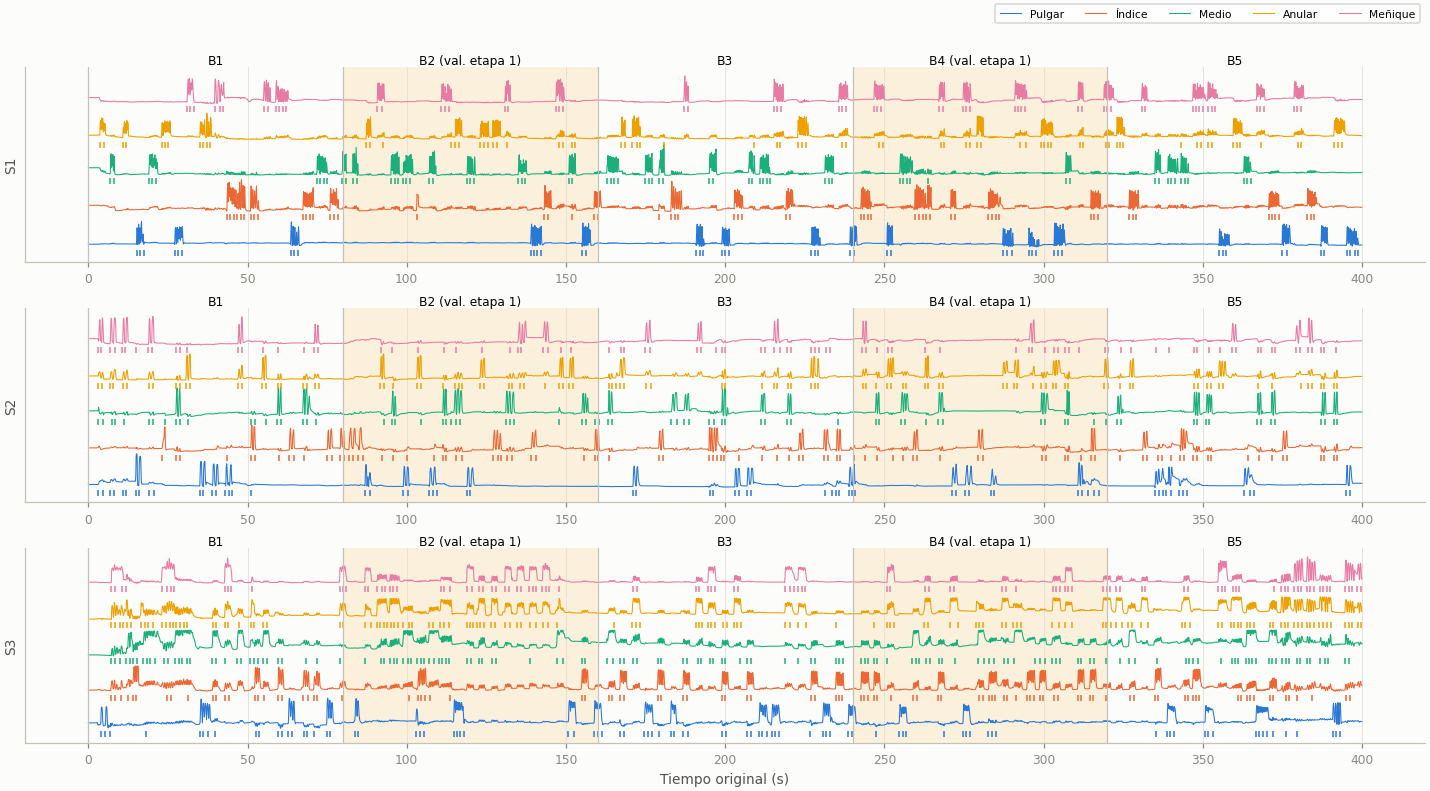
\includegraphics[width=\linewidth,height=0.47\textheight,keepaspectratio]{imgs/s11_blocks_timeline.png}
      \figcap{1}{Divisi\'on de la se\~nal en cinco bloques cronol\'ogicos (\texttt{B1--B5}) y zona de purga ($P=256$ muestras) empleada en todos los experimentos de TT2. \textbf{Fuente:} Obtenida del repositorio GitHub \cite{rodas_valencia_tpe_ecog}.}
    \end{column}
  \end{columns}

  \takeaway{Esta divisi\'on por bloques purgados garantiza que tanto las ablaciones arquitect\'onicas como la b\'usqueda en Optuna TPE eval\'uen la generalizaci\'on real sobre intervalos futuros no observados \cite{roberts2017crossvalidation,rodas_valencia_tpe_ecog}.}
\end{frame}


% 2. Exposición Principal — Evolución Arquitectónica A1-A5 y Optuna TPE (Diapositivas 6 a 9)
% =========================================================================
% MÓDULO 2: EVOLUCIÓN ARQUITECTÓNICA A1-A5 Y OPTUNA TPE (DIAPOSITIVAS 6 A 9)
% =========================================================================

% --- DIAPOSITIVA 6: EVOLUCIÓN ARQUITECTÓNICA EN TT2 (DE A0 A A5b Y A5) ---
\begin{frame}{Evoluci\'on Arquitect\'onica en TT2: De \texttt{A0} hasta \texttt{A5b} y \texttt{A5}}{Cuatro modificaciones estructurales acopladas sobre la l\'inea base de TT1 \cite{ronneberger2015unet,rodas_valencia_tpe_ecog}}
  \centering
  \scriptsize
  \renewcommand{\arraystretch}{1.18}
  \setlength{\tabcolsep}{4.5pt}
  \begin{tabularx}{\textwidth}{@{} l l l >{\raggedright\arraybackslash}X @{}}
    \toprule
    \rowcolor{ipnDark}
    \textcolor{white}{\textbf{Variante}} &
    \textcolor{white}{\textbf{Eje de Redise\~no}} &
    \textcolor{white}{\textbf{Operador / Configuraci\'on}} &
    \textcolor{white}{\textbf{Efecto T\'ecnico y Ganancia en CV (\'Epoca 50)}} \\
    \midrule
    \textbf{\texttt{A0} (Base TT1)} & Punto de partida & \texttt{BatchNorm1d}, \texttt{Dropout} $0.30$ & L\'inea base inicial de referencia ($\mathbf{0.5489}$). \\
    \rowcolor{rowLight}
    \textbf{\texttt{A1}} & Normalizaci\'on & \textbf{\texttt{LayerNorm}} por instante $t$ & Elimina dependencia de estad\'isticas de lote ($\mathbf{+0.0605}$). \\
    \textbf{\texttt{A2}} & Regularizaci\'on & \textbf{\texttt{Dropout}} $0.30 \rightarrow \mathbf{0.10}$ & Conserva detalles finos de la envolvente ($\mathbf{+0.0110}$ aislado). \\
    \rowcolor{rowLight}
    \textbf{\texttt{A3}} & Sobremuestreo aislado & \texttt{ConvTranspose1d} sin \texttt{A1/A2/A4} & Inestable por s\'i sola; cae a $0.5173$ ($\mathbf{-0.0316}$ vs.\ \texttt{A0}). \\
    \textbf{\texttt{A4}} & Fusi\'on en Decoder & \textbf{\texttt{Up} $\to$ \texttt{Concat(skip)} $\to$ \texttt{Conv}} & Filtra conjuntamente el mapa sobremuestreado y el \textit{skip}. \\
    \rowcolor{rowLight}
    \textbf{\texttt{A5b}} & Integraci\'on lineal & \texttt{A1} + \texttt{A2} + \texttt{A4} + \textbf{Interp.\ Lineal} & Sobremuestreo fijo libre de pesos ($\mathbf{0.6779}$, $+0.1290$). \\
    \rowcolor{rowHighlight}
    \textbf{\texttt{A5} (Propuesta)} & Integraci\'on completa & \texttt{A1} + \texttt{A2} + \texttt{A4} + \textbf{\texttt{ConvTranspose1d} DW} & Sobremuestreo aprendible por canal (\texttt{groups}$=C$, $-99.8\%$ params vs.\ densa; alcanza $\mathbf{0.6837}$, $\mathbf{+0.1349}$). \\
    \bottomrule
  \end{tabularx}
  \fuente{Creaci\'on propia, obtenida del repositorio GitHub \cite{rodas_valencia_tpe_ecog}.}

  \takeaway{La convoluci\'on transpuesta \textit{depthwise} (\texttt{groups}$=C$) en \texttt{A5} a\~nade solo $4C$ pesos por nivel ($2048$ vs.\ $1\,048\,576$ en el nivel $8f$), evitando la sobreparametrizaci\'on y logrando la mayor fidelidad al acoplarse con \texttt{LayerNorm} y el nuevo orden del Decoder \cite{rodas_valencia_tpe_ecog}.}
\end{frame}

% --- DIAPOSITIVA 7: ENTRENAMIENTO, FUNCIÓN DE PÉRDIDA Y PARADA TEMPRANA ---
\begin{frame}{Entrenamiento, Funci\'on de P\'erdida H\'ibrida y Parada Temprana}{Alineaci\'on simult\'anea de amplitud y fase temporal en trayectorias continuas \cite{wang2025dtcnet,loshchilov2019decoupled,rodas_valencia_tpe_ecog}}
  \begin{columns}[T,onlytextwidth]
    \begin{column}{0.49\textwidth}
      \begin{block}{1. Funci\'on de P\'erdida H\'ibrida Compuesta}
        \scriptsize
        Para evitar predicciones planas cercanas a la media, la funci\'on objetivo pondera en partes iguales el error de escala ($\operatorname{MSE}$) y la distancia coseno temporal ($\mathcal{L}_{\text{cos}}$) \cite{wang2025dtcnet,Sliwowski2022}:
        \[
          \mathcal{L}(\mathbf{Y}, \hat{\mathbf{Y}}) = 0.5\,\operatorname{MSE}(\mathbf{Y}, \hat{\mathbf{Y}}) + 0.5\big(1 - \operatorname{CosSim}_{\text{temp}}(\mathbf{Y}, \hat{\mathbf{Y}})\big)
        \]
        \begin{itemize}\setlength{\itemsep}{2pt}
          \item $\operatorname{MSE}$: Penaliza desviaciones de amplitud absoluta en $[0,1]$.
          \item $1 - \operatorname{CosSim}_{\text{temp}}$: Maximiza directamente la correlaci\'on morfol\'ogica y la sincron\'ia de fase de los picos de flexi\'on.
        \end{itemize}
      \end{block}
    \end{column}

    \begin{column}{0.47\textwidth}
      \begin{block}{2. Optimizador \texttt{Adam} con $L_2$ Acoplada}
        \scriptsize
        \begin{itemize}\setlength{\itemsep}{3pt}
          \item \textbf{Regla de actualizaci\'on:} \texttt{Adam} est\'andar con penalizaci\'on $L_2$ acoplada en el gradiente ($\tilde{g}_i = \nabla_{w_i}\mathcal{L} + \lambda w_i$) \cite{loshchilov2019decoupled}.
          \item \textbf{Estabilidad num\'erica:} Tama\~no de lote $B=128$ y recorte de norma global de gradiente $\|\mathbf{g}\|_2 \le 1.0$.
        \end{itemize}
      \end{block}

      \begin{alertblock}{3. Pol\'itica de \textit{Early Stopping}}
        \scriptsize
        Selecci\'on del mejor \textit{checkpoint} de validaci\'on bajo la regla:
        \[
          \text{min\_epochs} = 15, \quad \text{patience} = 10, \quad \text{max\_epochs} = 50
        \]
      \end{alertblock}
    \end{column}
  \end{columns}
\end{frame}

% --- DIAPOSITIVA 8: OPTIMIZACIÓN BAYESIANA MEDIANTE OPTUNA TPE ---
\begin{frame}{Optimizaci\'on Bayesiana mediante Optuna TPE}{B\'usqueda conjunta de arquitectura e hiperpar\'ametros adaptada por sujeto \cite{Bergstra2011,akiba2019optuna,rodas_valencia_tpe_ecog}}
  \begin{columns}[T,onlytextwidth]
    \begin{column}{0.47\textwidth}
      \begin{block}{Muestreador TPE en Optuna}
        \scriptsize
        \begin{itemize}\setlength{\itemsep}{3pt}
          \item El estimador \textit{Tree-structured Parzen Estimator} (TPE) modela dos densidades sobre el historial ($\gamma = 0.25$) \cite{Bergstra2011,akiba2019optuna}:
            \begin{itemize}\scriptsize
              \item $\ell(\bm{\lambda})$: Configuraciones en el cuartil superior.
              \item $g(\bm{\lambda})$: Configuraciones restantes.
            \end{itemize}
          \item Maximiza la mejora esperada seleccionando candidatos que maximizan el cociente $\ell(\bm{\lambda}) / g(\bm{\lambda})$.
          \item \textbf{Funci\'on objetivo por sujeto $s$:}
            \[
              J(\bm{\lambda}, s) = \frac{1}{5}\sum_{k=1}^{5}\left[\max_{e \in E_{s,k,\bm{\lambda}}} r_{s,k,e}^{\text{val}}\right]
            \]
        \end{itemize}
      \end{block}
    \end{column}

    \begin{column}{0.49\textwidth}
      \begin{block}{Espacio de B\'usqueda Mixto ($\Lambda$) y Presupuesto}
        \scriptsize
        \centering
        \renewcommand{\arraystretch}{1.2}
        \setlength{\tabcolsep}{2.8pt}
        \begin{tabular}{@{} l l l @{}}
          \toprule
          \rowcolor{ipnDark}
          \textcolor{white}{\textbf{Hiperpar\'ametro}} &
          \textcolor{white}{\textbf{Escala}} &
          \textcolor{white}{\textbf{Dominio Explorado}} \\
          \midrule
          \texttt{architecture\_id} & Categ\'orica & $\{\texttt{A5},\; \texttt{A5b}\}$ \\
          \rowcolor{rowLight}
          Learning rate ($\eta$) & Log-continua & $[5\times 10^{-5},\; 5\times 10^{-4}]$ \\
          Regularizaci\'on $L_2$ ($\lambda$) & Log-continua & $[10^{-7},\; 10^{-3}]$ \\
          \rowcolor{rowLight}
          Tama\~no de kernel ($k$) & Categ\'orica & $\{5,\; 7\}$ \\
          Niveles U-Net ($L$) & Entera & $\{4,\; 5\}$ \\
          \rowcolor{rowLight}
          Canales base ($f$) & Categ\'orica & $\{64,\; 96\}$ \\
          \bottomrule
        \end{tabular}
        \fuente{Creaci\'on propia, obtenida del repositorio GitHub \cite{rodas_valencia_tpe_ecog}.}
        \vspace{1mm}

        {\scriptsize\textbf{Presupuesto 100\% completado:} $32\text{ trials/sujeto}$ ($10$ \textit{warmups} balanceados $5\text{ \texttt{A5}}/5\text{ \texttt{A5b}} + 22\text{ TPE}$) $\times 5\text{ folds} = \mathbf{480\text{ entrenamientos}}$.}
      \end{block}
    \end{column}
  \end{columns}
\end{frame}

% --- DIAPOSITIVA 9: DINÁMICA DE EXPLORACIÓN EN OPTUNA TPE ---
\begin{frame}{Din\'amica de Exploraci\'on y Capacidad en Optuna TPE}{Evoluci\'on de los 32 ensayos por sujeto y relaci\'on entre n\'umero de par\'ametros y objetivo CV \cite{akiba2019optuna,rodas_valencia_tpe_ecog}}
  \begin{columns}[T,onlytextwidth]
    \begin{column}{0.48\textwidth}
      \centering
      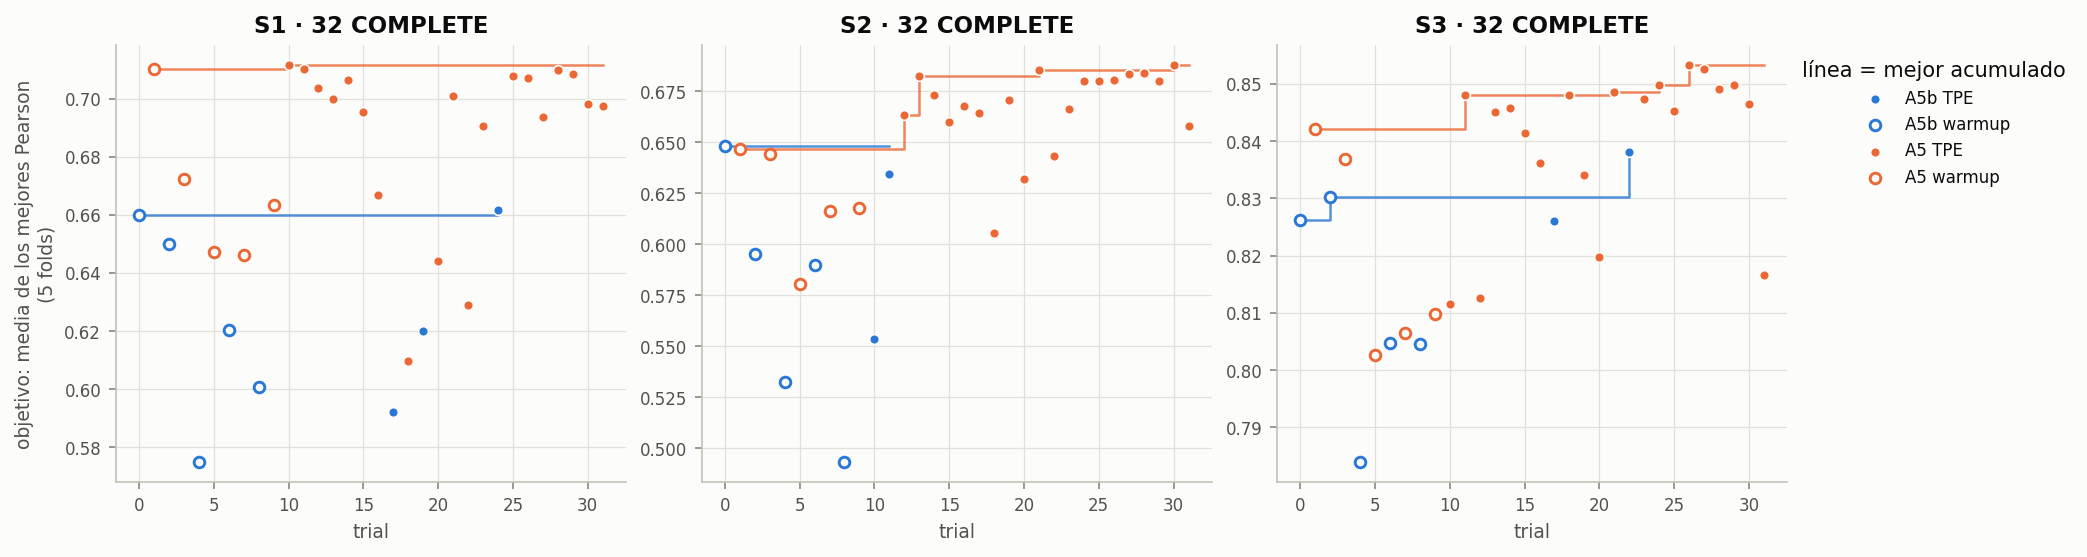
\includegraphics[width=\linewidth,height=0.47\textheight,keepaspectratio]{imgs/optimization_history.png}
      \figcap{2}{Historial de optimizaci\'on a lo largo de los $32$ ensayos por sujeto ($96$ trials totales) en Optuna TPE. \textbf{Fuente:} Obtenida del repositorio GitHub \cite{rodas_valencia_tpe_ecog}.}
    \end{column}
    \begin{column}{0.48\textwidth}
      \centering
      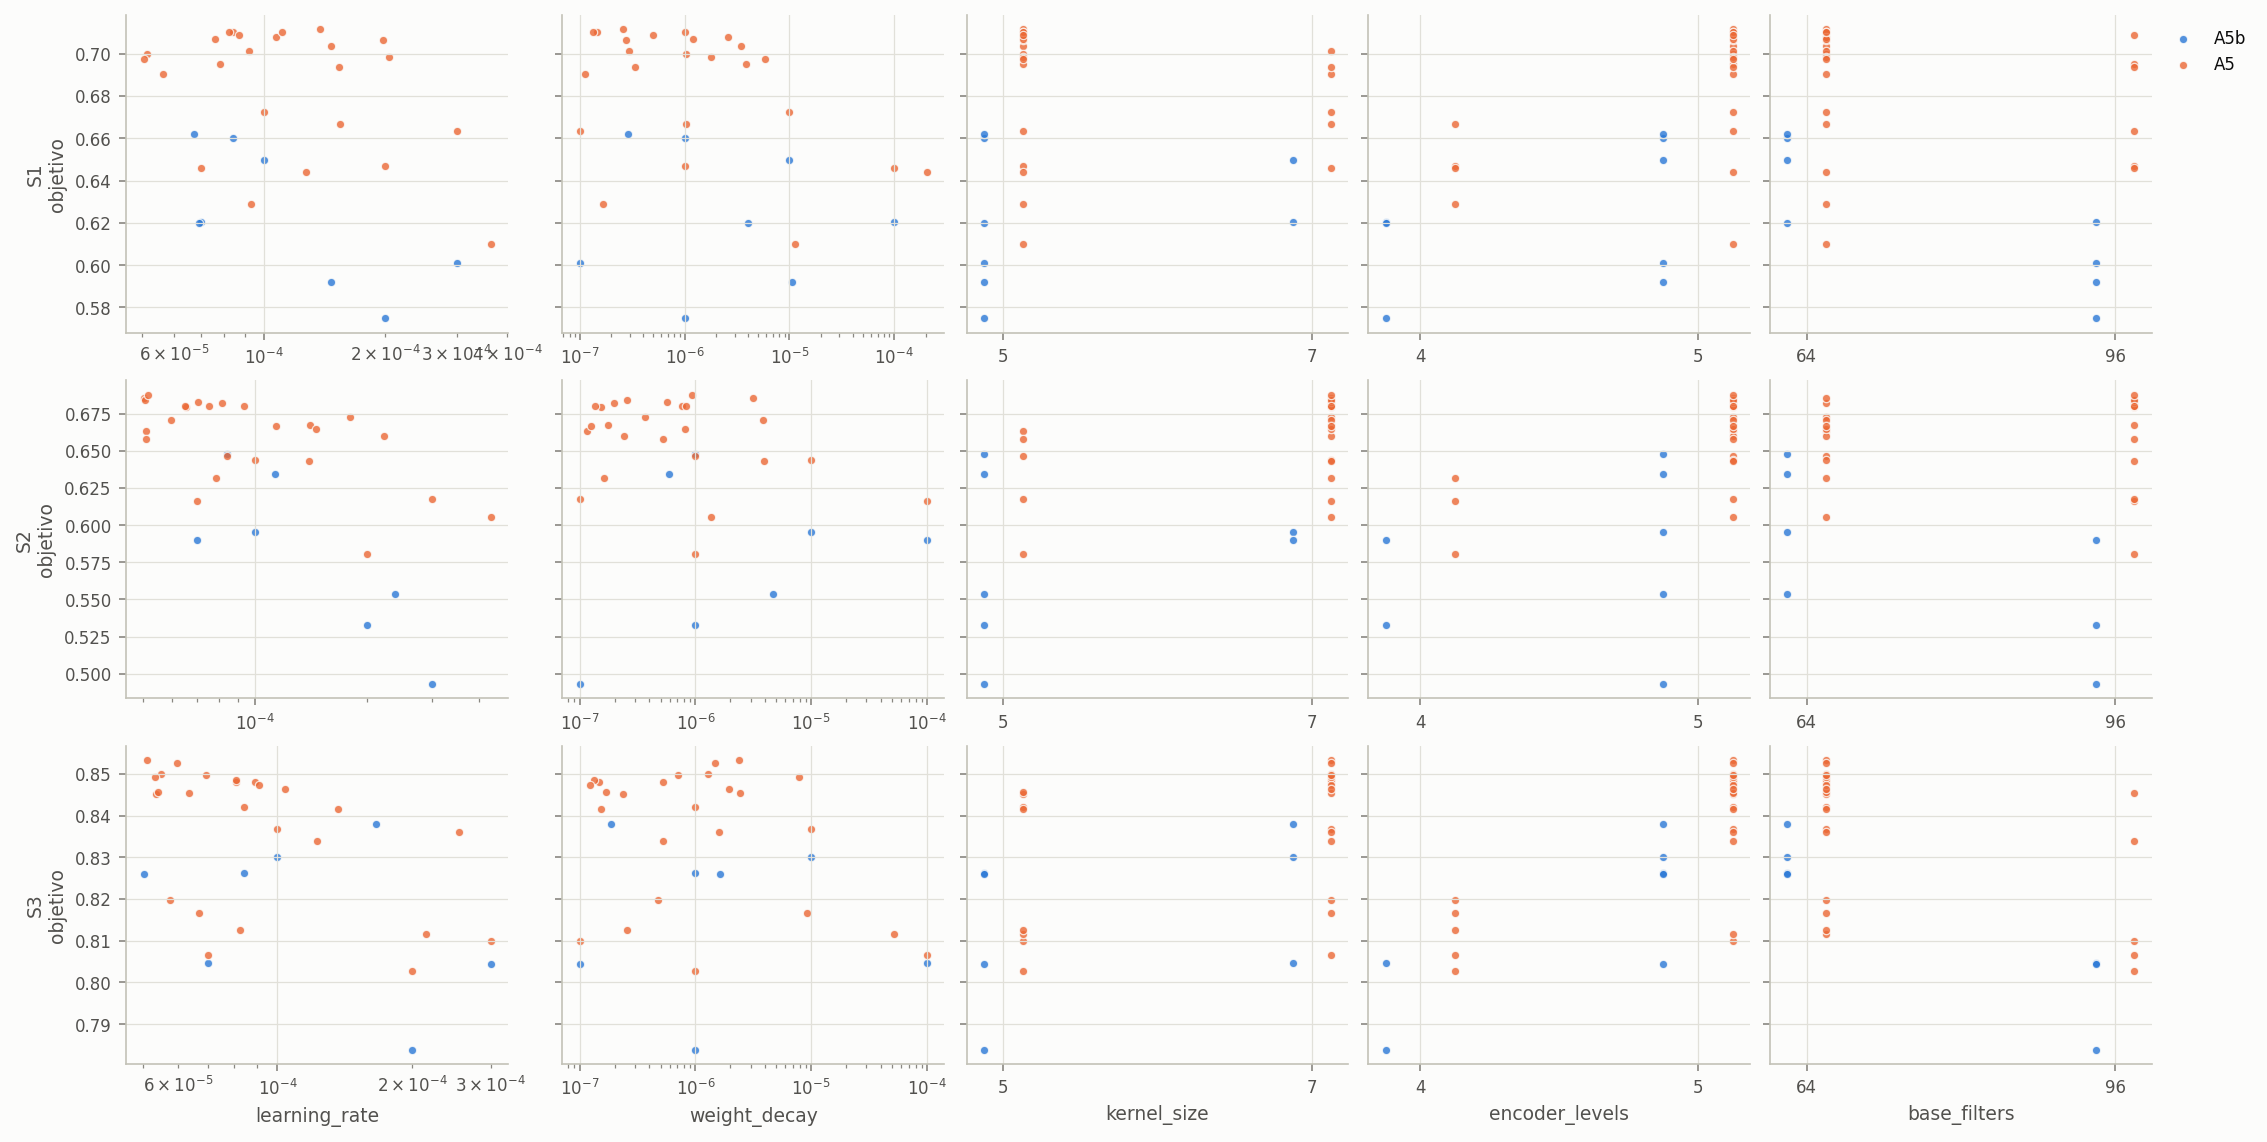
\includegraphics[width=\linewidth,height=0.47\textheight,keepaspectratio]{imgs/params_vs_objective.png}
      \figcap{3}{Relaci\'on entre complejidad param\'etrica ($N_{\text{params}}$), familia arquitect\'onica (\texttt{A5} vs.\ \texttt{A5b}) y correlaci\'on CV. \textbf{Fuente:} Obtenida del repositorio GitHub \cite{rodas_valencia_tpe_ecog}.}
    \end{column}
  \end{columns}

  \takeaway{En \texttt{S1} y \texttt{S3} las redes moderadas ($f=64$, $9.35\text{--}12.71\text{ M}$ params) saturan tempranamente el techo de validaci\'on, mientras que en el paciente m\'as complejo (\textbf{\texttt{S2}}) TPE identifica una mejora clara al escalar hacia mayor capacidad representacional ($k=7, L=5, f=96$, $28.03\text{ M}$ params) \cite{rodas_valencia_tpe_ecog}.}
\end{frame}


% 3. Exposición Principal — Resultados en 5 Etapas, Trayectorias y SOTA (Diapositivas 10 a 18)
% =========================================================================
% MÓDULO 3: RESULTADOS EN 5 ETAPAS, TRAYECTORIAS Y SOTA (DIAPOSITIVAS 10 A 18)
% =========================================================================

% --- DIAPOSITIVA 10: MAPA GENERAL DE LAS CINCO ETAPAS EXPERIMENTALES ---
\begin{frame}{Dise\~no Experimental y Mapa de las Cinco Etapas}{Trazabilidad de los 723 entrenamientos bajo preprocesamiento fijo \texttt{P0} \cite{rodas_valencia_tpe_ecog}}
  \scriptsize
  \centering
  \renewcommand{\arraystretch}{1.28}
  \setlength{\tabcolsep}{4.5pt}
  \begin{tabularx}{\textwidth}{@{} l c c c c >{\raggedright\arraybackslash}X @{}}
    \toprule
    \rowcolor{ipnDark}
    \textcolor{white}{\textbf{Etapa Experimental (\texttt{P0} fijo)}} &
    \textcolor{white}{\textbf{S1}} &
    \textcolor{white}{\textbf{S2}} &
    \textcolor{white}{\textbf{S3}} &
    \textcolor{white}{\textbf{Media}} &
    \textcolor{white}{\textbf{Aporte e Interpretaci\'on Metodol\'ogica}} \\
    \midrule
    \textbf{1.\ \texttt{A0} Base (CV \'ep.\ 50)} & $0.4990$ & $0.4289$ & $0.7187$ & $\mathbf{0.5489}$ & L\'inea base inicial de referencia ($15$ fits). \\
    \rowcolor{rowLight}
    \textbf{2.\ \texttt{A5} sin TPE (CV \'ep.\ 50)} & $0.6038$ & $0.6216$ & $0.8258$ & $\mathbf{0.6837}$ & $\mathbf{+0.1349}$ por redise\~no arquitect\'onico ($14/15$ folds $>0$). \\
    \textbf{2b.\ \texttt{A5} sin TPE (\textit{Checkpoint*})} & $0.7103$ & $0.6466$ & $0.8422$ & $\mathbf{0.7330}$ & $\mathbf{+0.0493}$ por parada temprana sobre hist\'oricos sin TPE. \\
    \rowcolor{rowLight}
    \textbf{3.\ \texttt{A5} con TPE (Mejor trial CV)} & $0.7117$ & $0.6878$ & $0.8533$ & $\mathbf{0.7509}$ & $\mathbf{+0.0179}$ durante la b\'usqueda en Optuna ($480$ fits). \\
    \textbf{4.\ \texttt{A5} Verificada (Semillas nuevas)} & $0.6929$ & $0.6785$ & $0.8402$ & $\mathbf{0.7372}$ & $\mathbf{+0.0041}$ neto global vs.\ 2b; $\mathbf{+0.0319}$ en \texttt{S2} ($60$ fits). \\
    \midrule
    \rowcolor{rowLight}
    \textbf{5a.\ \texttt{A5} Test Inicial (\texttt{B1--B4})} & $0.6087$ & $0.5226$ & $0.7685$ & $\mathbf{0.6333}$ & Evaluaci\'on inicial en prueba con parada en \texttt{B5} ($9$ fits). \\
    \rowcolor{rowHighlight}
    \textbf{5b.\ \texttt{A5} Test Oficial (\texttt{B1--B5})} & $\mathbf{0.6723}$ & $\mathbf{0.5490}$ & $\mathbf{0.7796}$ & $\mathbf{0.6669}$ & $\mathbf{+0.0337}$ al reentrenar con los 5 bloques ($9/9 > 0$). \\
    \bottomrule
  \end{tabularx}
  \fuente{Creaci\'on propia a partir del protocolo experimental implementado en GitHub \cite{rodas_valencia_tpe_ecog}.}

  \takeaway{Todas las correlaciones se calculan sobre la trayectoria continua reconstruida con \textit{overlap-add}, promediando los 5 dedos, los 5 bloques en CV y las \textbf{3 semillas completas en Test} (\texttt{3042, 4042, 5042}) sin elegir la mejor semilla \cite{rodas_valencia_tpe_ecog}.}
\end{frame}

% --- DIAPOSITIVA 11: ETAPAS 1 Y 2: ABLACIONES ARQUITECTÓNICAS ---
\begin{frame}{Etapas 1 y 2: Campa\~na de Ablaciones Arquitect\'onicas}{Impacto cuantitativo de las variantes sobre 165 entrenamientos controlados \cite{rodas_valencia_tpe_ecog}}
  \begin{columns}[c,onlytextwidth]
    \begin{column}{0.40\textwidth}
      \begin{block}{Resultados Clave de Ablaci\'on}
        \scriptsize
        \begin{itemize}\setlength{\itemsep}{3.5pt}
          \item \textbf{Mayor salto interno ($\mathbf{+0.1349}$):} Pasar de \texttt{A0} ($0.5489$) a \texttt{A5} ($0.6837$) en \'epoca 50 mejora \textbf{$14$ de los $15$ pliegues} (\texttt{S2} gana $\mathbf{+0.1927}$; \'unica excepci\'on \texttt{S1-B3} con $-0.0359$).
          \item \textbf{Lecci\'on de \texttt{A3} ($0.5173$):} Usar \texttt{ConvTranspose1d} de forma aislada degrad\'o $-0.0316$. Su ventaja emerge solo al combinarse con \texttt{LayerNorm} (\texttt{A1}: $+0.0605$) y el nuevo orden del Decoder en \texttt{A5}.
          \item \textbf{Control experimental:} Se mantuvo fijo el preprocesamiento \texttt{P0} en las etapas posteriores para aislar sin confusi\'on el aporte de \texttt{A5} y TPE.
        \end{itemize}
      \end{block}
    \end{column}

    \begin{column}{0.57\textwidth}
      \centering
      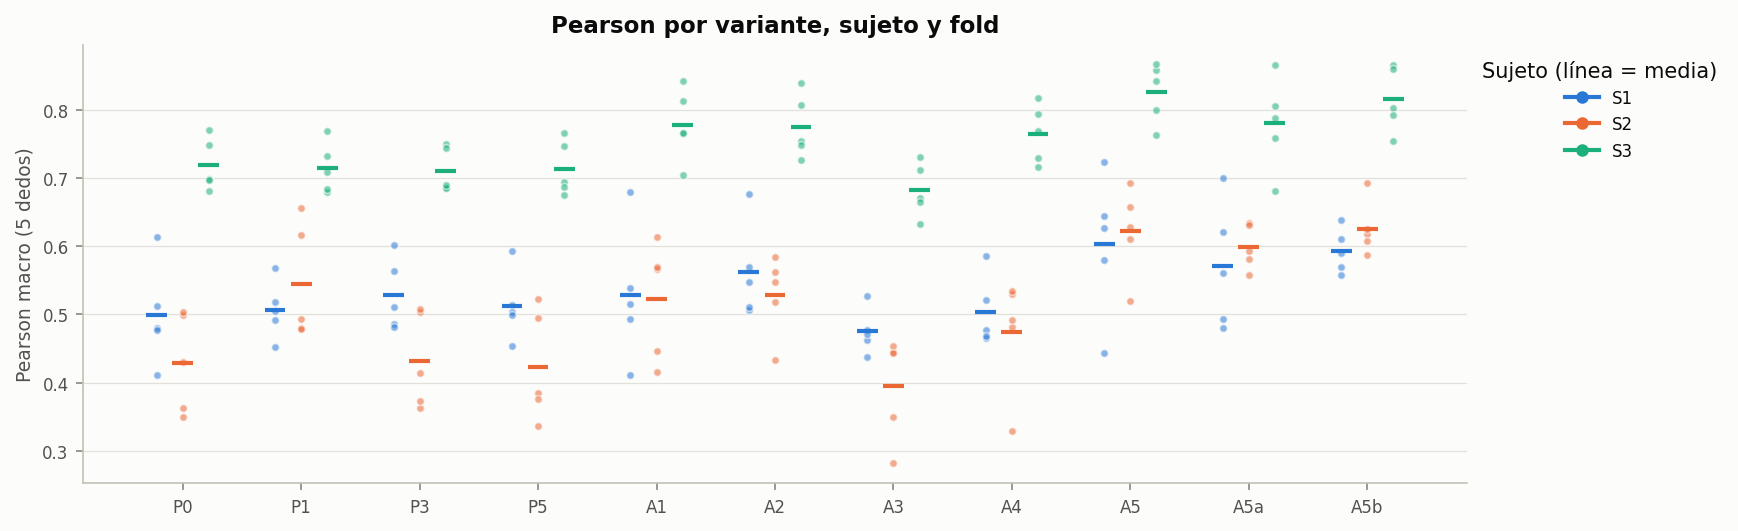
\includegraphics[width=\linewidth,height=0.49\textheight,keepaspectratio]{imgs/pearson_by_variant.png}
      \figcap{4}{Correlaci\'on de Pearson macro por variante (\texttt{P0--P5} y \texttt{A1--A5b}), sujeto y pliegue en la \'epoca 50. \textbf{Fuente:} Obtenida del repositorio GitHub \cite{rodas_valencia_tpe_ecog}.}
    \end{column}
  \end{columns}

  \takeaway{El redise\~no arquitect\'onico acoplado ($\texttt{A0} \to \texttt{A5}$) constituye el factor individual de mayor impacto en todo el proyecto, superando ampliamente el efecto posterior del ajuste fino de hiperpar\'ametros \cite{rodas_valencia_tpe_ecog}.}
\end{frame}

% --- DIAPOSITIVA 12: DINÁMICA DE CONVERGENCIA Y SELECCIÓN DE CHECKPOINT ---
\begin{frame}{Din\'amica de Convergencia y Selecci\'on de \textit{Checkpoint}}{Desacoplamiento del efecto de parada temprana ($+0.0493$) antes de aplicar Optuna TPE \cite{cawley2010overfitting,rodas_valencia_tpe_ecog}}
  \begin{columns}[c,onlytextwidth]
    \begin{column}{0.40\textwidth}
      \begin{block}{Puente Metodol\'ogico 2b}
        \scriptsize
        \begin{itemize}\setlength{\itemsep}{3.5pt}
          \item \textbf{Sobreajuste al final de las 50 \'epocas:} Las curvas de validaci\'on alcanzan su m\'aximo entre las \'epocas $18$ y $35$, degrad\'andose ligeramente hacia la \'epoca $50$.
          \item \textbf{Efecto puro del \textit{checkpoint} ($\mathbf{+0.0493}$):} Evaluar los mismos entrenamientos hist\'oricos de \texttt{A5} sin TPE con la regla de parada temprana ($\text{min}=15, \text{patience}=10$) eleva la media de $0.6837$ a $\mathbf{0.7330}$.
          \item \textbf{Impacto por sujeto:} \texttt{S1} sube $\mathbf{+0.1066}$ ($0.6038 \to 0.7103$), \texttt{S2} $+0.0250$ y \texttt{S3} $+0.0164$.
        \end{itemize}
      \end{block}
    \end{column}

    \begin{column}{0.57\textwidth}
      \centering
      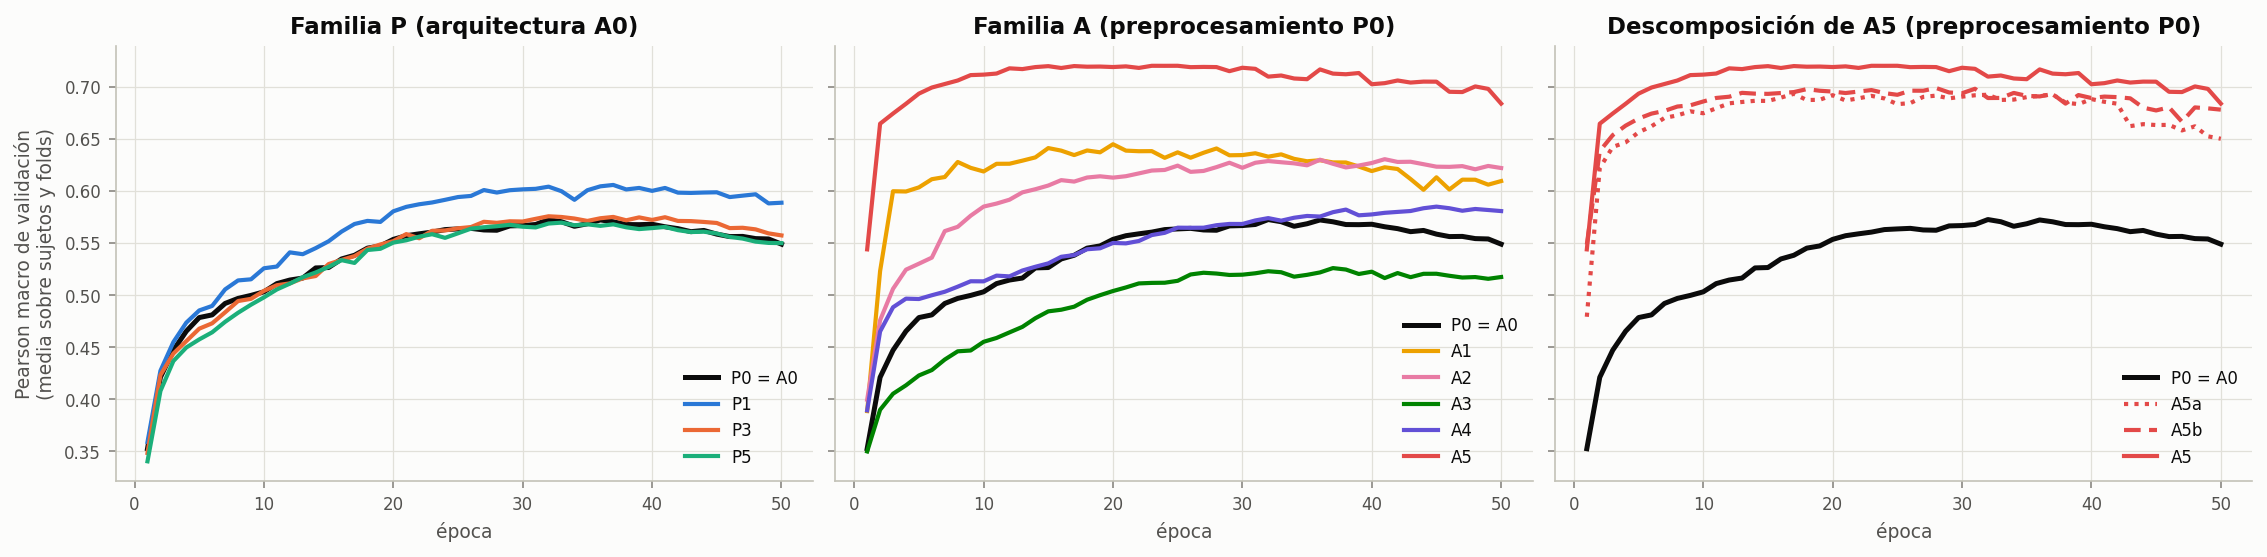
\includegraphics[width=\linewidth,height=0.52\textheight,keepaspectratio]{imgs/training_curves.png}
      \figcap{5}{Evoluci\'on de la correlaci\'on de validaci\'on por \'epoca para las familias \texttt{P}, \texttt{A} y la descomposici\'on hacia \texttt{A5}. \textbf{Fuente:} Obtenida del repositorio GitHub \cite{rodas_valencia_tpe_ecog}.}
    \end{column}
  \end{columns}

  \takeaway{Cuantificar este escal\'on de $\mathbf{+0.0493}$ evita un error metodol\'ogico com\'un: atribuir falsamente a la optimizaci\'on bayesiana una ganancia que en realidad proviene de seleccionar el mejor \textit{checkpoint} temporal \cite{cawley2010overfitting}.}
\end{frame}

% --- DIAPOSITIVA 13: ETAPAS 3 Y 4: BÚSQUEDA TPE Y VERIFICACIÓN MULTI-SEMILLA ---
\begin{frame}{Etapas 3 y 4: B\'usqueda TPE y Verificaci\'on Multi-Semilla}{Control del optimismo de b\'usqueda con 60 entrenamientos sobre semillas nuevas \cite{cawley2010overfitting,rodas_valencia_tpe_ecog}}
  \begin{columns}[c,onlytextwidth]
    \begin{column}{0.41\textwidth}
      \begin{block}{Auditor\'ia Estad\'istica de TPE}
        \scriptsize
        \begin{itemize}\setlength{\itemsep}{3pt}
          \item \textbf{Etapa 3 (Mejor Trial TPE = $\mathbf{0.7509}$):} Frente a \texttt{A5} con \textit{checkpoint} ($0.7330$), la b\'usqueda aporta $\mathbf{+0.0179}$ en la media ($\text{S2}$ sube $+0.0413$).
          \item \textbf{Etapa 4 (Verificaci\'on con 2 semillas nuevas/fold = $60$ fits):}
            \begin{itemize}\scriptsize
              \item \textbf{\texttt{A5} ($\mathbf{0.7372}$) supera a \texttt{A5b} ($0.7112$)} por $\mathbf{+0.0260}$ con mejoras en los 3 sujetos.
              \item Al descontar el sesgo del m\'aximo \cite{cawley2010overfitting}, la ganancia global sobre $0.7330$ es marginal ($\mathbf{+0.0041}$), pero \textbf{se mantiene un beneficio real en \texttt{S2} ($\mathbf{+0.0319}$)}.
            \end{itemize}
        \end{itemize}
      \end{block}
    \end{column}

    \begin{column}{0.56\textwidth}
      \centering
      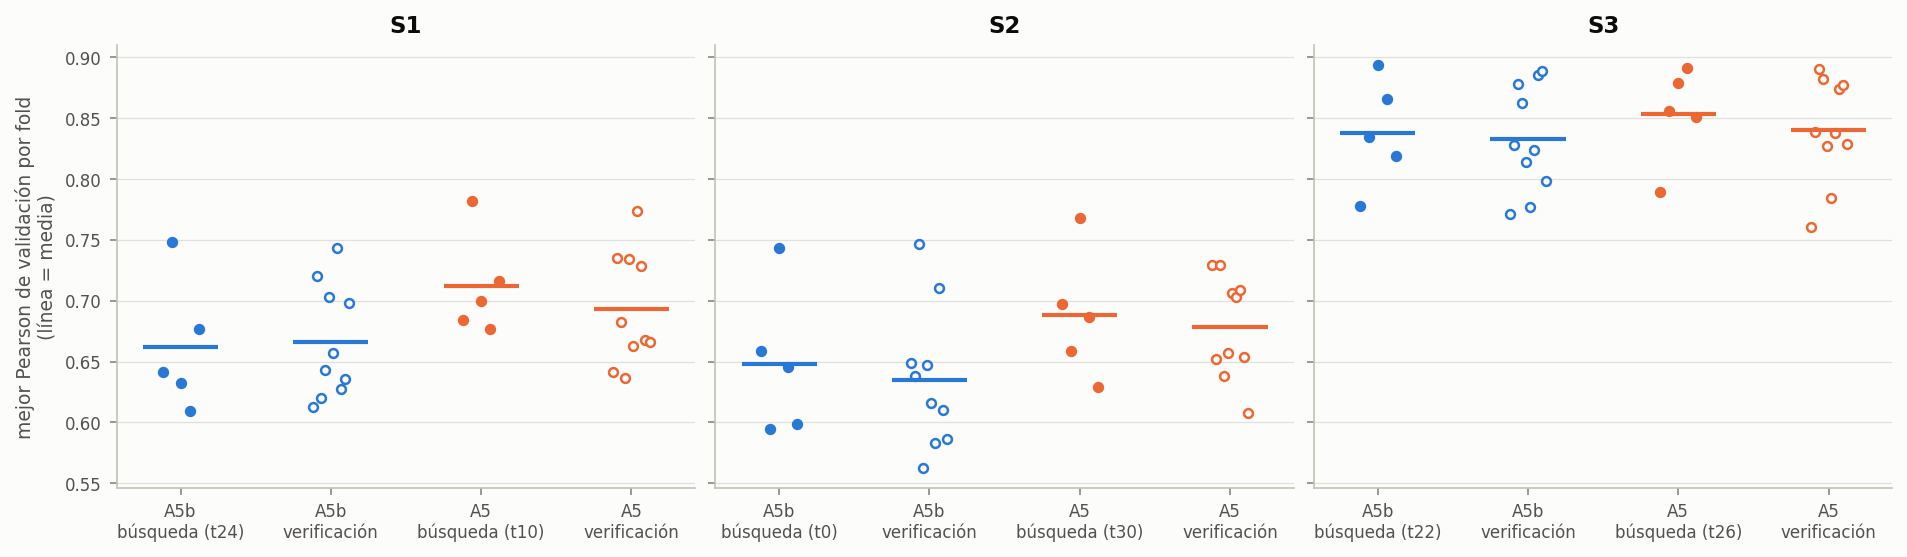
\includegraphics[width=\linewidth,height=0.52\textheight,keepaspectratio]{imgs/verification.png}
      \figcap{6}{Contraste entre el puntaje de b\'usqueda TPE y la verificaci\'on con semillas independientes para \texttt{A5} y \texttt{A5b} en los 3 sujetos. \textbf{Fuente:} Obtenida del repositorio GitHub \cite{rodas_valencia_tpe_ecog}.}
    \end{column}
  \end{columns}

  \takeaway{La verificaci\'on multi-semilla demostr\'o que \texttt{S1} y \texttt{S3} ya operaban cerca de su techo con hiperpar\'ametros base, mientras que TPE fue determinante para rescatar el desempe\~no del \textbf{Sujeto 2} ($+0.0319$) y confirmar la superioridad de \texttt{A5} sobre \texttt{A5b} \cite{rodas_valencia_tpe_ecog}.}
\end{frame}

% --- DIAPOSITIVA 14: CONFIGURACIONES SELECCIONADAS Y REGLA DE ÉPOCAS FIJAS ---
\begin{frame}{Configuraciones Seleccionadas por Sujeto y Regla de \'Epocas Fijas}{Modelos ganadores de la familia \texttt{A5} y protocolo de transici\'on al conjunto de prueba \cite{rodas_valencia_tpe_ecog}}
  \scriptsize
  \centering
  \renewcommand{\arraystretch}{1.35}
  \setlength{\tabcolsep}{5.5pt}
  \begin{tabularx}{\textwidth}{@{} l c c c c c c >{\raggedright\arraybackslash}X @{}}
    \toprule
    \rowcolor{ipnDark}
    \textcolor{white}{\textbf{Sujeto}} &
    \textcolor{white}{\textbf{Trial}} &
    \textcolor{white}{\textbf{Kernel $k$}} &
    \textcolor{white}{\textbf{Niveles $L$}} &
    \textcolor{white}{\textbf{Canales $f$}} &
    \textcolor{white}{\textbf{Par\'ametros}} &
    \textcolor{white}{\textbf{Verif.\ CV}} &
    \textcolor{white}{\textbf{Horizonte Fijo Test (\texttt{B1--B5})}} \\
    \midrule
    \textbf{\texttt{S1}} & Trial 10 & $k = 5$ & $L = 5$ & $f = 64$ & $\mathbf{9.35\text{ M}}$ & $0.6929 \pm 0.0566$ & $\mathbf{21\text{ \'epocas}}$ ($\eta = 1.38\times 10^{-4}$) \\
    \rowcolor{rowHighlight}
    \textbf{\texttt{S2}} & Trial 30 & $k = 7$ & $L = 5$ & $f = 96$ & $\mathbf{28.03\text{ M}}$ & $0.6785 \pm 0.0680$ & $\mathbf{32\text{ \'epocas}}$ ($\eta = 5.16\times 10^{-5}$) \\
    \textbf{\texttt{S3}} & Trial 26 & $k = 7$ & $L = 5$ & $f = 64$ & $\mathbf{12.71\text{ M}}$ & $0.8402 \pm 0.0369$ & $\mathbf{28\text{ \'epocas}}$ ($\eta = 5.10\times 10^{-5}$) \\
    \midrule
    \rowcolor{rowLight}
    \textbf{Media} & --- & --- & --- & --- & $16.70\text{ M}$ & $\mathbf{0.7372}$ & Mediana de $10$ corridas de verif. \\
    \bottomrule
  \end{tabularx}
  \fuente{Creaci\'on propia, obtenida del repositorio GitHub \cite{rodas_valencia_tpe_ecog}.}

  \vspace{1.5mm}
  \begin{columns}[T,onlytextwidth]
    \begin{column}{0.48\textwidth}
      \begin{block}{Protocolo Inicial \texttt{b1b4\_es\_b5}}
        \scriptsize
        Entrena sobre los bloques \texttt{B1--B4} ($80\%$ de los datos) y utiliza el bloque \texttt{B5} como validaci\'on interna para parada temprana. Desaprovecha el bloque m\'as cercano al conjunto de prueba.
      \end{block}
    \end{column}
    \begin{column}{0.48\textwidth}
      \begin{alertblock}{Protocolo Reentrenado \texttt{b1b5\_fixed}}
        \scriptsize
        Integra el $\mathbf{100\%}$ \textbf{de los bloques de desarrollo (\texttt{B1--B5})} entrenando durante la mediana exacta de \'epocas verificadas ($21, 32\text{ y }28$), sin observar jam\'as el bloque de prueba oficial.
      \end{alertblock}
    \end{column}
  \end{columns}
\end{frame}

% --- DIAPOSITIVA 15: ETAPA 5: EVALUACIÓN EN EL CONJUNTO DE PRUEBA OFICIAL ---
\begin{frame}{Etapa 5: Evaluaci\'on en el Conjunto de Prueba Oficial}{Desempe\~no final auditado sobre las tres semillas independientes (\texttt{3042, 4042, 5042}) \cite{lin1989concordance,rodas_valencia_tpe_ecog}}
  \begin{columns}[c,onlytextwidth]
    \begin{column}{0.49\textwidth}
      \scriptsize
      \centering
      \renewcommand{\arraystretch}{1.24}
      \setlength{\tabcolsep}{2.8pt}
      \begin{tabular}{@{} l c c c c @{}}
        \toprule
        \rowcolor{ipnDark}
        \textcolor{white}{\textbf{Suj.}} &
        \textcolor{white}{\textbf{\texttt{B1--B4}}} &
        \textcolor{white}{\textbf{\texttt{B1--B5} (Test)}} &
        \textcolor{white}{\textbf{CCC}} &
        \textcolor{white}{\textbf{MSE}} \\
        \midrule
        \textbf{\texttt{S1}} & $0.6087$ & $\mathbf{0.6723 \pm 0.0009}$ & $0.5534$ & $0.6497$ \\
        \rowcolor{rowLight}
        \textbf{\texttt{S2}} & $0.5226$ & $\mathbf{0.5490 \pm 0.0143}$ & $0.4050$ & $0.8667$ \\
        \textbf{\texttt{S3}} & $0.7685$ & $\mathbf{0.7796 \pm 0.0069}$ & $0.7694$ & $0.3606$ \\
        \midrule
        \rowcolor{rowHighlight}
        \textbf{Media} & $\mathbf{0.6333}$ & $\mathbf{0.6669}$ ($\mathbf{+0.0337}$) & $\mathbf{0.5759}$ & $\mathbf{0.6257}$ \\
        \bottomrule
      \end{tabular}
      \fuente{Creaci\'on propia, obtenida del repositorio GitHub \cite{rodas_valencia_tpe_ecog}.}

      \vspace{1.2mm}
      \begin{block}{Consistencia en las 9 Ejecuciones}
        \scriptsize
        \begin{itemize}\setlength{\itemsep}{2pt}
          \item El protocolo \texttt{b1b5\_fixed} supera a \texttt{b1b4\_es\_b5} en las \textbf{$9/9$ parejas sujeto-semilla} ($+0.0635$ en \texttt{S1}, $+0.0264$ en \texttt{S2}, $+0.0111$ en \texttt{S3}).
          \item Mejora simult\'aneamente el $\operatorname{CCC}$ de Lin ($0.5210 \to \mathbf{0.5759}$) y reduce el $\operatorname{MSE}$ ($0.6597 \to \mathbf{0.6257}$) \cite{lin1989concordance}.
        \end{itemize}
      \end{block}
    \end{column}

    \begin{column}{0.48\textwidth}
      \centering
      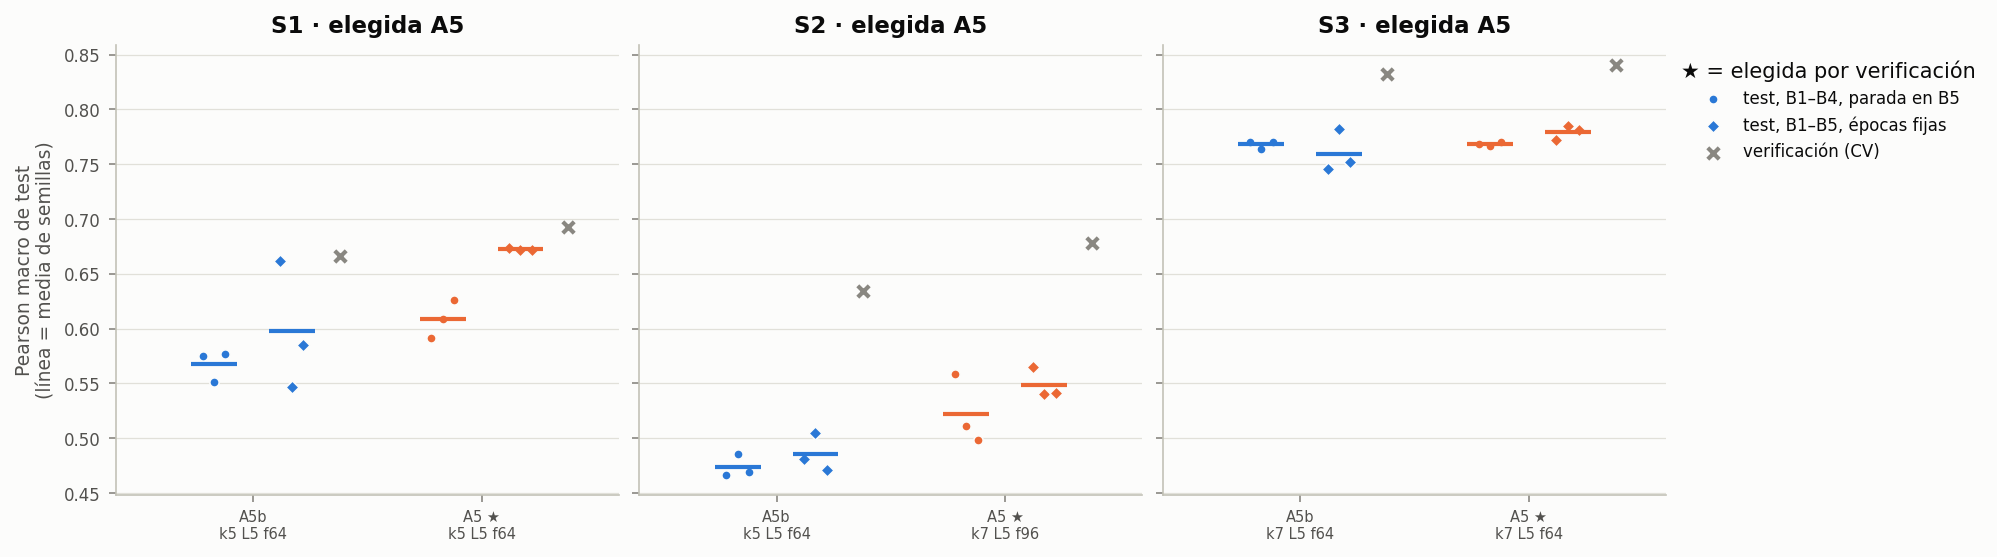
\includegraphics[width=\linewidth,height=0.50\textheight,keepaspectratio]{imgs/test_scores.png}
      \figcap{7}{Puntajes en el conjunto de prueba oficial por sujeto y semilla: protocolo inicial (\texttt{B1--B4}) frente a reentrenamiento completo (\texttt{B1--B5}). \textbf{Fuente:} Obtenida del repositorio GitHub \cite{rodas_valencia_tpe_ecog}.}
    \end{column}
  \end{columns}

  \takeaway{Por transparencia metodol\'ogica se reportan siempre ambas cifras: $0.6333$ como primera evaluaci\'on en prueba y $\mathbf{0.6669}$ como resultado del protocolo reentrenado sobre los 5 bloques \cite{rodas_valencia_tpe_ecog}.}
\end{frame}

% --- DIAPOSITIVA 16: ANÁLISIS DE RESULTADOS POR SUJETO Y POR DEDO ---
\begin{frame}{An\'alisis de Resultados por Sujeto y por Dedo}{Desempe\~no individual de los cinco dedos e interpretaci\'on biomec\'anica \cite{rodas_valencia_tpe_ecog}}
  \begin{columns}[c,onlytextwidth]
    \begin{column}{0.46\textwidth}
      \scriptsize
      \centering
      \renewcommand{\arraystretch}{1.22}
      \setlength{\tabcolsep}{3.2pt}
      \begin{tabular}{@{} l c c c c @{}}
        \toprule
        \rowcolor{ipnDark}
        \textcolor{white}{\textbf{Dedo}} &
        \textcolor{white}{\textbf{S1}} &
        \textcolor{white}{\textbf{S2}} &
        \textcolor{white}{\textbf{S3}} &
        \textcolor{white}{\textbf{Media Test}} \\
        \midrule
        \rowcolor{rowHighlight}
        \textbf{1.\ Anular} & $0.7429$ & $0.6431$ & $0.7745$ & $\mathbf{0.7202}$ \\
        \rowcolor{rowLight}
        \textbf{2.\ \'Indice} & $0.7525$ & $0.6197$ & $0.7760$ & $\mathbf{0.7161}$ \\
        \textbf{3.\ Pulgar} & $0.6777$ & $0.5835$ & $0.8130$ & $\mathbf{0.6914}$ \\
        \rowcolor{rowLight}
        \textbf{4.\ Me\~nique} & $0.6085$ & $0.4918$ & $0.7982$ & $\mathbf{0.6328}$ \\
        \textbf{5.\ Medio} & $0.5798$ & $0.4107$ & $0.7322$ & $\mathbf{0.5742}$ \\
        \midrule
        \textbf{Media Sujeto} & $\mathbf{0.6723}$ & $\mathbf{0.5490}$ & $\mathbf{0.7796}$ & $\mathbf{0.6669}$ \\
        \bottomrule
      \end{tabular}
      \fuente{Creaci\'on propia, obtenida del repositorio GitHub \cite{rodas_valencia_tpe_ecog}.}

      \vspace{1.5mm}
      \begin{block}{Patr\'on Somatot\'opico y Biomec\'anico}
        \scriptsize
        \begin{itemize}\setlength{\itemsep}{2pt}
          \item \textbf{Anular ($0.7202$) e \'Indice ($0.7161$)} presentan la mayor fidelidad de reconstrucci\'on en los 3 sujetos.
          \item El \textbf{dedo Medio ($0.5742$)} constituye el mayor reto ($\text{S2}=0.4107$) por su fuerte coactivaci\'on tendinosa y solapamiento cortical con los dedos adyacentes.
        \end{itemize}
      \end{block}
    \end{column}

    \begin{column}{0.51\textwidth}
      \centering
      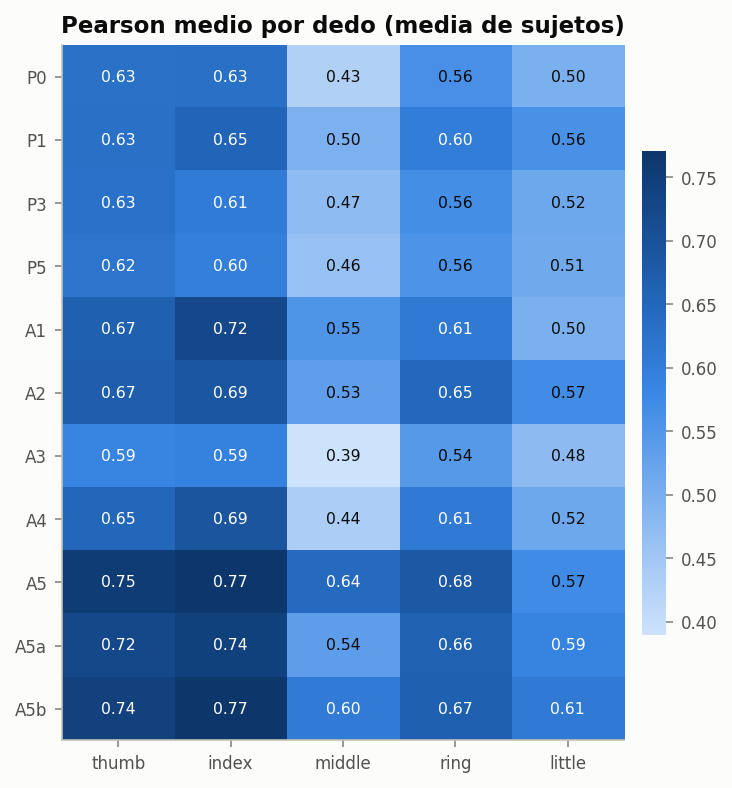
\includegraphics[width=\linewidth,height=0.52\textheight,keepaspectratio]{imgs/pearson_per_finger.png}
      \figcap{8}{Mapa de calor de correlaci\'on de Pearson por dedo a trav\'es de las variantes evaluadas (media de los tres sujetos). \textbf{Fuente:} Obtenida del repositorio GitHub \cite{rodas_valencia_tpe_ecog}.}
    \end{column}
  \end{columns}
\end{frame}

% --- DIAPOSITIVA 17: DEMOSTRACIÓN DE TRAYECTORIAS CONTINUAS Y AUDITORÍA V01-V14 ---
\begin{frame}{Demostraci\'on de Trayectorias Continuas y Auditor\'ia \texttt{V01--V14}}{Comparaci\'on visual del seguimiento cinem\'atico y verificaci\'on de integridad del software \cite{rodas_valencia_tpe_ecog}}
  \begin{columns}[T,onlytextwidth]
    \begin{column}{0.48\textwidth}
      \centering
      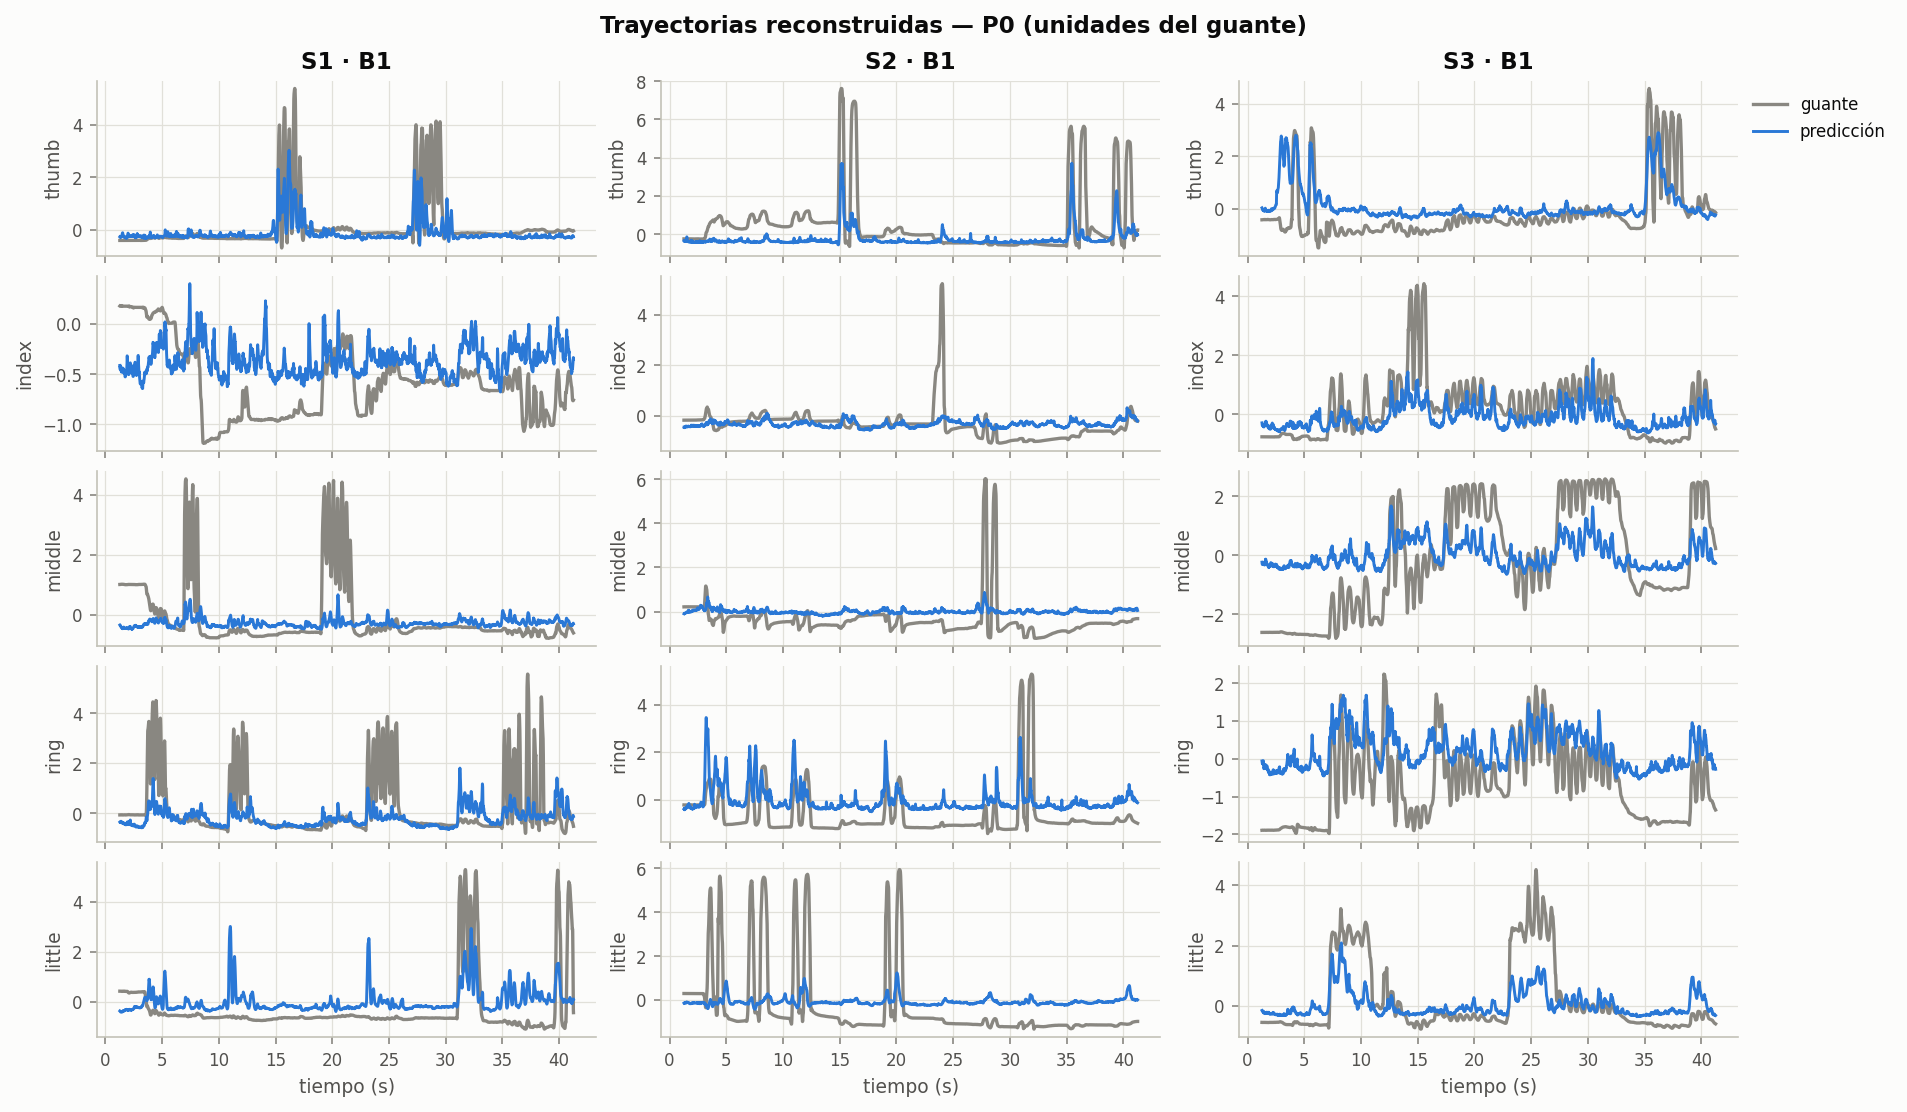
\includegraphics[width=\linewidth,height=0.45\textheight,keepaspectratio]{imgs/example_predictions_P0.png}
      \figcap{9}{\textbf{Modelo Base \texttt{A0/P0} ($0.5489$ CV):} predicciones con oscilaciones espurias. \textbf{Fuente:} Obtenida del repositorio GitHub \cite{rodas_valencia_tpe_ecog}.}
    \end{column}
    \begin{column}{0.48\textwidth}
      \centering
      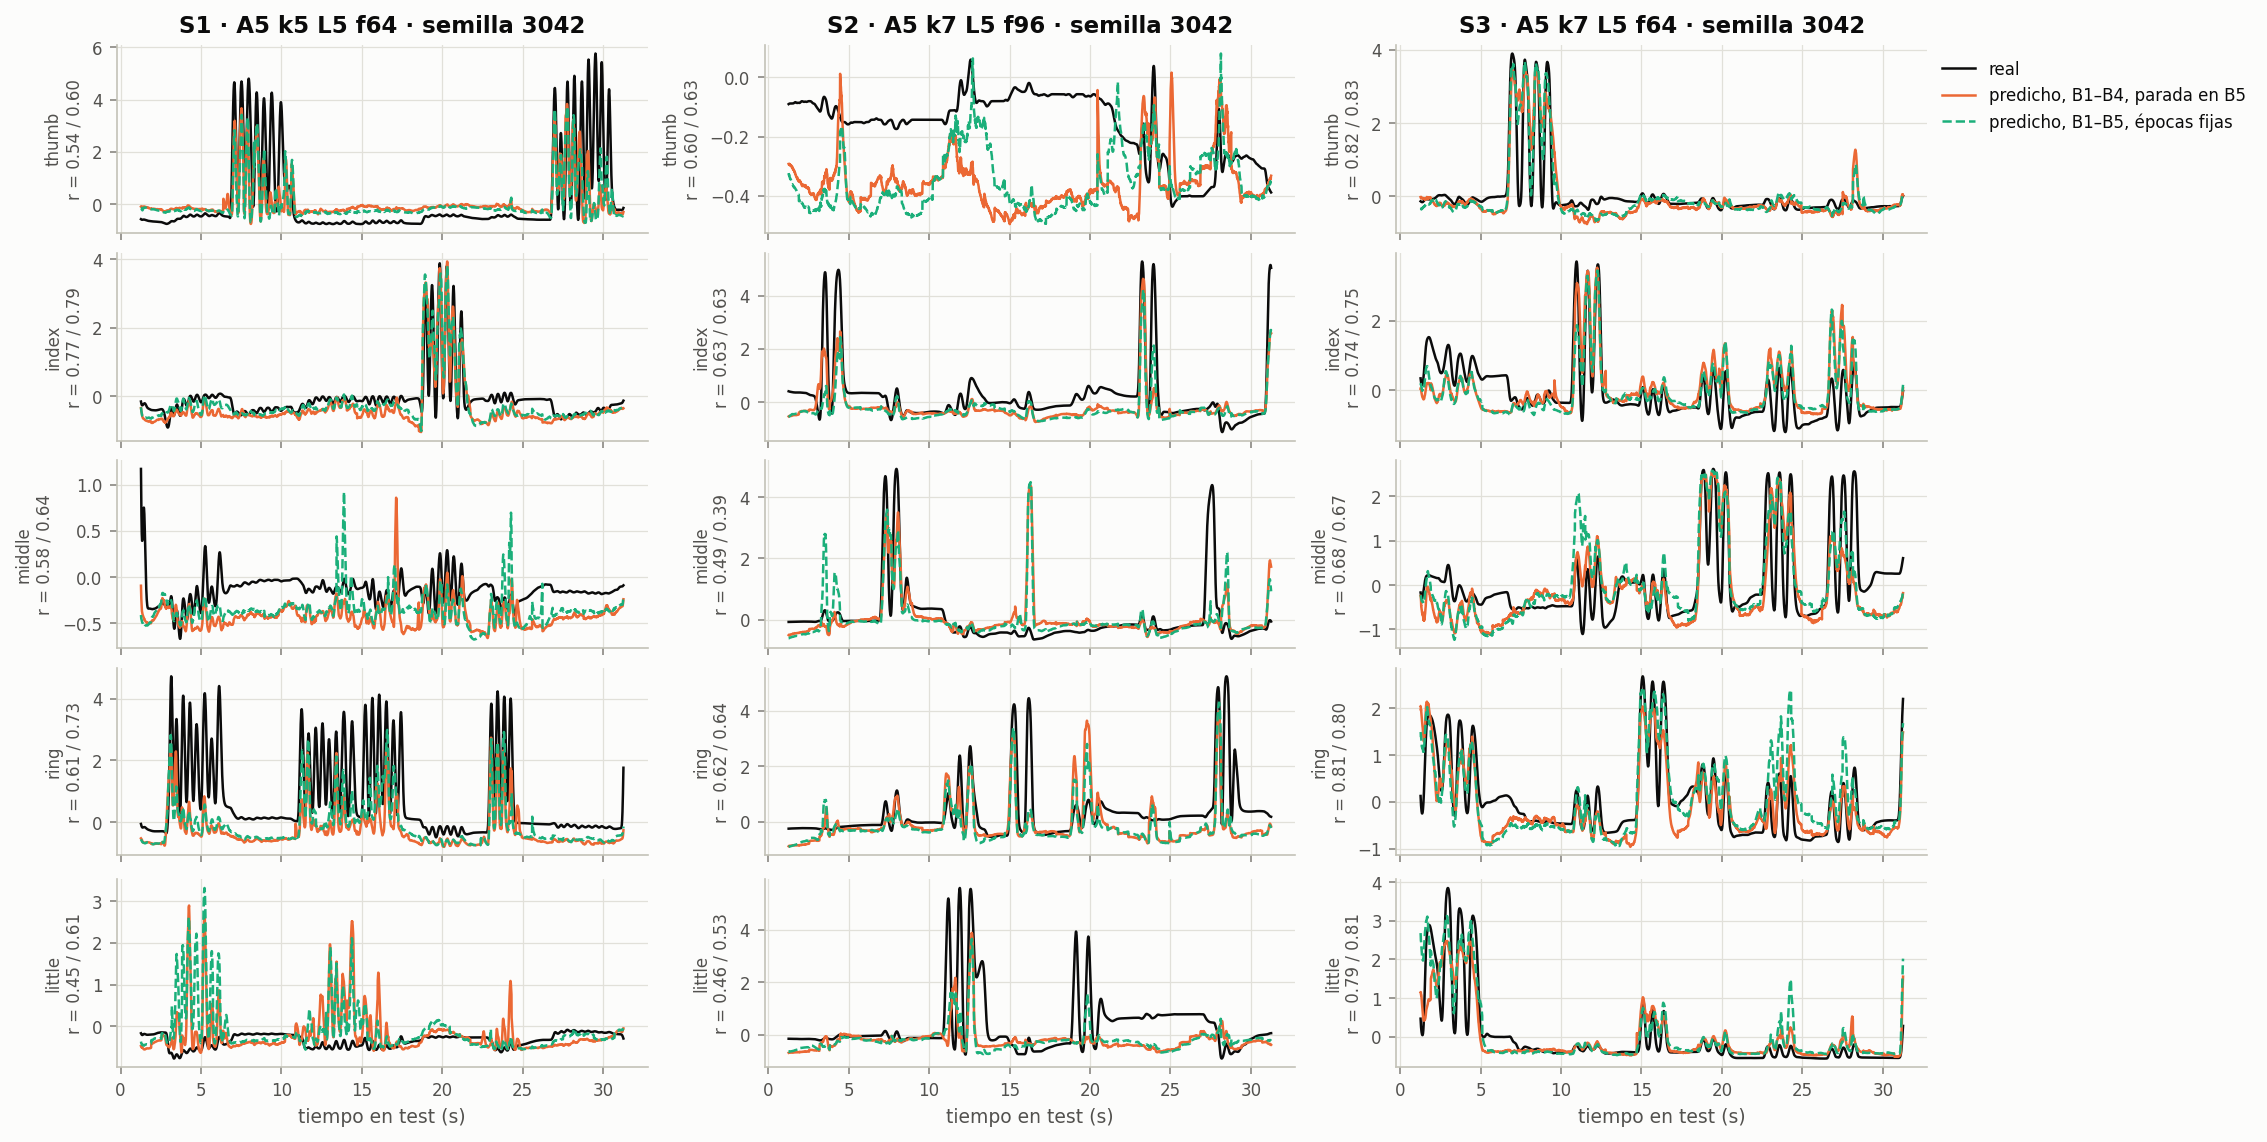
\includegraphics[width=\linewidth,height=0.45\textheight,keepaspectratio]{imgs/test_trajectories.png}
      \figcap{10}{\textbf{Modelo Final \texttt{A5} en Test Oficial ($0.6669$):} seguimiento preciso de flexi\'on y reposo. \textbf{Fuente:} Obtenida del repositorio GitHub \cite{rodas_valencia_tpe_ecog}.}
    \end{column}
  \end{columns}

  \takeaway{\textbf{Auditor\'ia Automatizada (\texttt{14/14 PASS}):} Las compuertas \texttt{V01--V14} y el manifiesto SHA-256 (\texttt{b26db4c4...}) certifican cero solapamiento entre bloques, ajuste exclusivo de escaladores en entrenamiento y reproducibilidad determinista \cite{rodas_valencia_tpe_ecog}.}
\end{frame}

% --- DIAPOSITIVA 18: COMPARACIÓN CRÍTICA FRENTE AL ESTADO DEL ARTE ---
\begin{frame}{Comparaci\'on Cr\'itica frente al Estado del Arte}{Benchmark en el \textit{Dataset 4} de la \textit{BCI Competition IV} \cite{liang2012decoding,Xie2018,Lomtev2022,wang2025dtcnet,rodas_valencia_tpe_ecog}}
  \scriptsize
  \centering
  \renewcommand{\arraystretch}{1.20}
  \setlength{\tabcolsep}{5pt}
  \begin{tabularx}{\textwidth}{@{} >{\raggedright\arraybackslash}X c c c c @{}}
    \toprule
    \rowcolor{ipnDark}
    \textcolor{white}{\textbf{M\'etodo / Arquitectura Reportada en Literatura}} &
    \textcolor{white}{\textbf{Sujeto 1}} &
    \textcolor{white}{\textbf{Sujeto 2}} &
    \textcolor{white}{\textbf{Sujeto 3}} &
    \textcolor{white}{\textbf{Promedio}} \\
    \midrule
    \textit{Switching linear model} (Liang \& Bougrain, 2012) \cite{liang2012decoding} & $0.48$ & $0.24$ & $0.56$ & $0.43$ \\
    \rowcolor{rowLight}
    \textit{Compact CNN} (2018) / \textit{Linear regression} (2017) & $0.45$ & $0.34$ & $0.56$ & $0.45\text{--}0.48$ \\
    \textit{CNN-LSTM} (Xie et al., 2018) \cite{Xie2018} / \textit{highGRM} (2022) & $0.55\text{--}0.56$ & $0.41\text{--}0.42$ & $0.58\text{--}0.61$ & $0.52\text{--}0.53$ \\
    \midrule
    \textbf{\textit{FingerFlex}} (U-Net 1D, Lomtev et al., 2022) \cite{Lomtev2022} & $0.64$ & $0.56$ & $0.73$ & $\mathbf{0.64}$ \\
    \rowcolor{rowLight}
    \textbf{\textit{DTCNet}} (Conv 3D dilatada, Wang et al., 2025) \cite{wang2025dtcnet} & $0.71$ & $0.59$ & $0.77$ & $\mathbf{0.69}$ \\
    \midrule
    \textbf{Nuestro Modelo Base \texttt{A0/P0}} (CV \'ep.\ 50) & $0.4990$ & $0.4289$ & $0.7187$ & $0.5489$ \\
    \rowcolor{rowLight}
    \textbf{Nuestro Modelo \texttt{A5}} (Test inicial \texttt{b1b4\_es\_b5}, 3 semillas) & $0.6087$ & $0.5226$ & $0.7685$ & $\mathbf{0.6333}$ \\
    \rowcolor{rowHighlight}
    \textbf{Nuestro Modelo \texttt{A5}} (Test reentrenado \texttt{b1b5\_fixed}, 3 semillas) & $\mathbf{0.6723}$ & $\mathbf{0.5490}$ & $\mathbf{0.7796}$ & $\mathbf{0.6669}$ \\
    \bottomrule
  \end{tabularx}
  \fuente{Creaci\'on propia a partir de \cite{liang2012decoding,Lomtev2022,wang2025dtcnet} y resultados del repositorio GitHub \cite{rodas_valencia_tpe_ecog}.}

  \vspace{1.5mm}
  \begin{columns}[T,onlytextwidth]
    \begin{column}{0.48\textwidth}
      \begin{block}{Superaci\'on de \textit{FingerFlex} \cite{Lomtev2022}}
        \scriptsize
        \texttt{A5} ($0.6669$) supera a la referencia directa U-Net 1D ($0.64$) en \textbf{\texttt{S1} ($+0.0323$), \texttt{S3} ($+0.0496$) y en la media global ($\mathbf{+0.0269}$)}.
      \end{block}
    \end{column}
    \begin{column}{0.48\textwidth}
      \begin{alertblock}{Contraste frente a \textit{DTCNet} \cite{wang2025dtcnet}}
        \scriptsize
        \texttt{A5} (1D) supera a \textit{DTCNet} (3D) en \textbf{\texttt{S3} ($0.7796$ vs.\ $0.77$), en el dedo Anular ($0.7202$ vs.\ $0.70$) y en $8/15$ celdas sujeto-dedo}; la brecha radica en el dedo Medio ($0.5742$ vs.\ $0.67$).
      \end{alertblock}
    \end{column}
  \end{columns}
\end{frame}


% 4. Conclusiones, Cumplimiento de Objetivos, Limitaciones y Trabajo Futuro (Diapositivas 19 a 22)
% =========================================================================
% MÓDULO 4: CONCLUSIONES, CUMPLIMIENTO, LIMITACIONES Y FUTURO (DIAPS. 19 A 22)
% =========================================================================

% --- DIAPOSITIVA 19: CONCLUSIONES GENERALES Y HALLAZGOS H1-H5 ---
\begin{frame}{Conclusiones Generales y Hallazgos Esenciales (\texttt{H1--H5})}{Desacoplamiento estad\'istico del aporte de arquitectura, \textit{checkpoint}, TPE y reentrenamiento \cite{rodas_valencia_tpe_ecog}}
  \begin{columns}[T,onlytextwidth]
    \begin{column}{0.48\textwidth}
      \begin{block}{Hallazgos sobre Arquitectura y HPO}
        \scriptsize
        \begin{itemize}\setlength{\itemsep}{1.5pt}
          \item \textbf{\texttt{H1} (Redise\~no Arquitect\'onico $\mathbf{+0.1349}$):} El paso de \texttt{A0} ($0.5489$) a \texttt{A5} ($0.6837$) con \texttt{LayerNorm}, menor \texttt{Dropout}, \textit{skip} previo y \texttt{ConvTranspose1d} \textit{depthwise} fue el avance m\'as determinante ($14/15$ folds positivos).
          \item \textbf{\texttt{H2} (Selecci\'on de \textit{Checkpoint} $\mathbf{+0.0493}$):} La parada temprana elev\'o \texttt{A5} sin TPE a $\mathbf{0.7330}$, separando el efecto temporal de la b\'usqueda de hiperpar\'ametros.
          \item \textbf{\texttt{H3} (Beneficio Espec\'ifico de TPE):} En verificaci\'on ($0.7372$), la mejora media fue marginal ($+0.0041$), pero result\'o \textbf{sustancial en el Sujeto 2 ($\mathbf{+0.0319}$)} y confirm\'o a \texttt{A5} sobre \texttt{A5b} ($+0.0260$).
        \end{itemize}
      \end{block}
    \end{column}

    \begin{column}{0.48\textwidth}
      \begin{alertblock}{Hallazgos en Prueba Oficial y Fisiolog\'ia}
        \scriptsize
        \begin{itemize}\setlength{\itemsep}{1.5pt}
          \item \textbf{\texttt{H4} (Reentrenamiento Completo $\mathbf{0.6669}$):} Integrar los 5 bloques (\texttt{B1--B5}) con la mediana de \'epocas verificadas super\'o al test inicial ($0.6333$) por $\mathbf{+0.0337}$ en las $9/9$ ejecuciones ($\operatorname{CCC}=0.5759$).
          \item \textbf{\texttt{H5} (Variabilidad Inter-Sujeto e Inter-Dedo):} Se mantiene una brecha anat\'omica entre sujetos ($\text{S3}=0.7796$ vs.\ $\text{S2}=0.5490$) y entre dedos (Anular $0.7202$ e \'Indice $0.7161$ frente al acoplamiento biomec\'anico del Medio $0.5742$).
        \end{itemize}
      \end{alertblock}
    \end{column}
  \end{columns}

  \takeaway{\textbf{Conclusi\'on central:} Las decisiones estructurales sobre la topolog\'ia de la red y la regla de selecci\'on temporal ejercen un impacto mayor que el ajuste fino de hiperpar\'ametros, el cual act\'ua como un adaptador clave para sujetos con menor relaci\'on se\~nal-ruido basal.}
\end{frame}

% --- DIAPOSITIVA 20: CUMPLIMIENTO DE OBJETIVOS (DOS TABLAS INDEPENDIENTES) ---
\begin{frame}{Evaluaci\'on del Cumplimiento de Objetivos}
  \scriptsize
  \centering
  \renewcommand{\arraystretch}{1.28}
  \setlength{\tabcolsep}{6pt}

  % Tabla 1. Cumplimiento del objetivo general
  {\footnotesize\bfseries\textcolor{ipnDark}{Tabla 1. Cumplimiento del objetivo general}\par}
  \vspace{1mm}
  \begin{tabularx}{\textwidth}{@{} >{\raggedright\arraybackslash}X c @{}}
    \toprule
    \rowcolor{ipnDark}
    \textcolor{white}{\textbf{Objetivo general}} &
    \textcolor{white}{\textbf{Estado de cumplimiento}} \\
    \midrule
    \rowcolor{rowLight}
    Desarrollar un marco de configuraci\'on basado en redes neuronales profundas para la decodificaci\'on continua de movimientos de dedos a partir de se\~nales electrocorticogr\'aficas del Dataset 4 de la BCI Competition IV, optimizando su arquitectura e hiperpar\'ametros mediante optimizaci\'on bayesiana y comparando su desempe\~no frente al modelo base y al estado del arte. & \cmark \\
    \bottomrule
  \end{tabularx}

  \vspace{3.5mm}

  % Tabla 2. Cumplimiento de los cuatro objetivos particulares
  {\footnotesize\bfseries\textcolor{ipnDark}{Tabla 2. Cumplimiento de los cuatro objetivos particulares}\par}
  \vspace{1mm}
  \begin{tabularx}{\textwidth}{@{} l >{\raggedright\arraybackslash}X c @{}}
    \toprule
    \rowcolor{ipnDark}
    \textcolor{white}{\textbf{Objetivo}} &
    \textcolor{white}{\textbf{Objetivo particular}} &
    \textcolor{white}{\textbf{Estado de cumplimiento}} \\
    \midrule
    \textbf{Objetivo Particular 1} & Implementar una metodolog\'ia de filtrado, segmentaci\'on, normalizaci\'on y extracci\'on espectral libre de fuga de informaci\'on temporal. & \cmark \\
    \rowcolor{rowLight}
    \textbf{Objetivo Particular 2} & Integrar el flujo continuo de modelado dise\~nando una arquitectura base y su evoluci\'on estructural para predecir trayectorias de flexi\'on. & \cmark \\
    \textbf{Objetivo Particular 3} & Dise\~nar e implementar con Optuna un esquema de optimizaci\'on bayesiana para buscar autom\'aticamente arquitecturas e hiperpar\'ametros por sujeto. & \cmark \\
    \rowcolor{rowLight}
    \textbf{Objetivo Particular 4} & Comparar el modelo optimizado frente al modelo base y al estado del arte bajo condiciones auditables. & \cmark \\
    \bottomrule
  \end{tabularx}
  \fuente{Creaci\'on propia a partir de los compromisos t\'ecnicos de la investigaci\'on \cite{rodas_valencia_tpe_ecog}.}
\end{frame}

% --- DIAPOSITIVA 21: RETOS Y LIMITACIONES DEL TRABAJO ---
\begin{frame}{Retos y Limitaciones del Trabajo y C\'omo se Afrontaron}{Transparencia metodol\'ogica y fronteras de inferencia cient\'ifica \cite{cawley2010overfitting,rodas_valencia_tpe_ecog}}
  \vfill
  \centering
  {\footnotesize
  \renewcommand{\arraystretch}{1.34}
  \setlength{\tabcolsep}{6pt}
  \begin{tabularx}{\textwidth}{@{} l >{\raggedright\arraybackslash}X >{\raggedright\arraybackslash}X @{}}
    \toprule
    \rowcolor{ipnDark}
    \textcolor{white}{\textbf{Reto o Limitaci\'on}} &
    \textcolor{white}{\textbf{Implicaci\'on Metodol\'ogica}} &
    \textcolor{white}{\textbf{Medida de Rigor Implementada}} \\
    \midrule
    \textbf{1.\ Muestra cl\'inica ($N=3$)} & Alta variabilidad inter-sujeto ($\text{S2}=0.5490$ a $\text{S3}=0.7796$) que impide inferencias poblacionales. & Reporte desglosado por paciente y dedo, aplicando b\'usqueda TPE personalizada por sujeto. \\
    \rowcolor{rowLight}
    \textbf{2.\ Optimismo en 32 trials TPE} & Seleccionar el m\'aximo de $32$ ensayos introduce sesgo de selecci\'on ($0.7509$) \cite{cawley2010overfitting}. & Ejecuci\'on de $60$ entrenamientos de verificaci\'on con semillas nuevas ($0.7372$) y separaci\'on del \textit{checkpoint} ($0.7330$). \\
    \textbf{3.\ Car\'acter de \texttt{b1b5\_fixed}} & El reentrenamiento con los 5 bloques se dise\~n\'o tras observar el primer test ($0.6333$). & Reporte conjunto de ambos protocolos ($0.6333$ inicial y $0.6669$ reentrenado) con \'epocas fijadas por mediana de CV. \\
    \rowcolor{rowLight}
    \textbf{4.\ Acoplamiento del dedo Medio} & Menor correlaci\'on en prueba ($0.5742$) frente a Anular ($0.7202$) e \'Indice ($0.7161$). & Evaluaci\'on individualizada por dedo en las 15 celdas sujeto-dedo frente al estado del arte. \\
    \bottomrule
  \end{tabularx}
  }
  \fuente{Creaci\'on propia \cite{cawley2010overfitting,rodas_valencia_tpe_ecog}.}
  \vfill
\end{frame}

% --- DIAPOSITIVA 22: TRABAJO FUTURO (EXCLUSIVAMENTE COMPRESIÓN EMBEBIDA) ---
\begin{frame}{Trabajo a Futuro: Optimizaci\'on para Sistemas Embebidos}{Estrategias de compresi\'on de modelos para reducir recursos computacionales \cite{Xie2026,rodas_valencia_tpe_ecog}}
  \begin{columns}[T,onlytextwidth]
    \begin{column}{0.48\textwidth}
      \begin{block}{1. Destilaci\'on de Conocimiento}
        \scriptsize
        \begin{itemize}\setlength{\itemsep}{4.5pt}
          \item \textbf{Transferencia maestro-estudiante (\textit{Knowledge Distillation}):} Transferir el conocimiento de los modelos \texttt{A5} ($9.35\text{ M}$ a $28.03\text{ M}$ de par\'ametros) a arquitecturas m\'as compactas \cite{Xie2026}.
          \item \textbf{Alineaci\'on de representaciones:} Entrenar la red ligera para reproducir tanto las trayectorias continuas de los cinco dedos como las activaciones latentes del decodificador.
          \item \textbf{Beneficio operativo:} Disminuir el costo de inferencia manteniendo la precisi\'on alcanzada en la prueba oficial ($r = 0.6669$).
        \end{itemize}
      \end{block}
    \end{column}

    \begin{column}{0.48\textwidth}
      \begin{alertblock}{2. Poda Estructurada de Par\'ametros y Canales}
        \scriptsize
        \begin{itemize}\setlength{\itemsep}{4pt}
          \item \textbf{Eliminaci\'on de filtros redundantes:} Reducir el tama\~no de las redes \texttt{A5} podando el $50\%$ de los canales en las etapas profundas $4f$ y $8f$ (que concentran $>72\%$ de los pesos).
          \item \textbf{Criterio de relevancia por canal:} Seleccionar filtros mediante la norma $\ell_1$ de los kernels y el factor de escala $\gamma_o$ de \texttt{LayerNorm}:
            \[
              \mathcal{I}_{\text{LN}}(o) = |\gamma_o| \cdot \|\mathbf{W}_{o,:,:}\|_2
            \]
          \item \textbf{Despliegue en sistemas embebidos:} Reducci\'on proyectada del $\mathbf{75\%}$ \textbf{en FLOPs y memoria} ($<3\text{ M}$ de par\'ametros) para neuropr\'otesis de bajo consumo.
        \end{itemize}
      \end{alertblock}
    \end{column}
  \end{columns}

  \takeaway{Ambas l\'ineas permiten trasladar el desempe\~no de las redes \texttt{A5} hacia hardware embebido con restricciones estrictas de memoria, c\'omputo y disipaci\'on t\'ermica \cite{Xie2026,rodas_valencia_tpe_ecog}.}
\end{frame}


% 5. Referencias Bibliográficas (Diapositivas 23 a 25)
% =========================================================================
% MÓDULO 6: REFERENCIAS BIBLIOGRÁFICAS COMPLETAS (DIAPOSITIVAS 29 A 31)
% =========================================================================
\bibslidetrue
\setbeamertemplate{bibliography item}[text]
\begin{frame}[allowframebreaks]{Referencias Bibliogr\'aficas}{Fuentes cient\'ificas, metodol\'ogicas y de estado del arte citadas en la presentaci\'on}
  \scriptsize
  \begin{thebibliography}{21}
    \setlength{\itemsep}{3.5pt}

    \bibitem{miller2008prediction}
    K.~J. Miller and G.~Schalk, ``Prediction of finger flexion: 4th {Brain-Computer Interface} data competition ({Dataset 4}),'' \emph{BCI Competition IV}, 2008. [Online]. Available: \url{https://www.bbci.de/competition/iv/desc_4.pdf}

    \bibitem{schalk2004bci2000}
    G.~Schalk, D.~J. McFarland, T.~Hinterberger, N.~Birbaumer, and J.~R. Wolpaw, ``{BCI2000}: A general-purpose brain-computer interface ({BCI}) system,'' \emph{IEEE Transactions on Biomedical Engineering}, vol.~51, no.~6, pp. 1034--1043, 2004.

    \bibitem{Schalk2011}
    G.~Schalk and E.~C. Leuthardt, ``Brain-computer interfaces using electrocorticographic signals,'' \emph{IEEE Reviews in Biomedical Engineering}, vol.~4, pp. 140--154, 2011.

    \bibitem{kaplan2019decoding}
    K.~Volkova, M.~A. Lebedev, A.~Kaplan, and A.~Ossadtchi, ``Decoding movement from electrocorticographic activity: A review,'' \emph{Frontiers in Neuroinformatics}, vol.~13, p.~74, 2019.

    \bibitem{Bundy2016}
    D.~T. Bundy, M.~Pahwa, N.~Szrama, and E.~C. Leuthardt, ``Decoding three-dimensional reaching movements using electrocorticographic signals in humans,'' \emph{Journal of Neural Engineering}, vol.~13, no.~2, p. 026021, 2016.

    \bibitem{gruenwald2023highgamma}
    J.~Gruenwald, S.~Sieghartsleitner, C.~Kapeller, J.~Scharinger, K.~Kamada, P.~Brunner, and C.~Guger, ``Characterization of high-gamma activity in electrocorticographic signals,'' \emph{Frontiers in Neuroscience}, vol.~17, p. 1206120, 2023.

    \bibitem{wirth2000crispdm}
    R.~Wirth and J.~Hipp, ``{CRISP-DM}: Towards a standard process model for data mining,'' in \emph{Proc. 4th Int. Conf. Practical Applications of Knowledge Discovery and Data Mining}, vol.~1, 2000, pp. 29--39.

    \framebreak

    \bibitem{roberts2017crossvalidation}
    D.~R. Roberts \emph{et~al.}, ``Cross-validation strategies for data with temporal, spatial, hierarchical, or phylogenetic structure,'' \emph{Ecography}, vol.~40, no.~8, pp. 913--929, 2017.

    \bibitem{ronneberger2015unet}
    O.~Ronneberger, P.~Fischer, and T.~Brox, ``{U-Net}: Convolutional networks for biomedical image segmentation,'' in \emph{Medical Image Computing and Computer-Assisted Intervention ({MICCAI})}, vol. 9351, Springer, 2015, pp. 234--241.

    \bibitem{Sliwowski2022}
    M.~Sliwowski, ``Artificial intelligence for real-time decoding of motor commands from {ECoG} of disabled subjects for chronic brain computer interfacing,'' Ph.D. dissertation, Universit\'e Grenoble Alpes, 2022.

    \bibitem{loshchilov2019decoupled}
    I.~Loshchilov and F.~Hutter, ``Decoupled weight decay regularization,'' in \emph{International Conference on Learning Representations ({ICLR})}, 2019, pp. 1--19.

    \bibitem{Bergstra2011}
    J.~Bergstra, R.~Bardenet, Y.~Bengio, and B.~K\'egl, ``Algorithms for hyper-parameter optimization,'' in \emph{Advances in Neural Information Processing Systems ({NeurIPS})}, vol.~24, 2011, pp. 2546--2554.

    \bibitem{akiba2019optuna}
    T.~Akiba, S.~Sano, T.~Yanase, T.~Ohta, and M.~Koyama, ``{Optuna}: A next-generation hyperparameter optimization framework,'' in \emph{Proc. 25th ACM SIGKDD Int. Conf. Knowledge Discovery \& Data Mining}, 2019, pp. 2623--2631.

    \bibitem{cawley2010overfitting}
    G.~C. Cawley and N.~L.~C. Talbot, ``On over-fitting in model selection and subsequent selection bias in performance evaluation,'' \emph{Journal of Machine Learning Research}, vol.~11, pp. 2079--2107, 2010.

    \framebreak

    \bibitem{lin1989concordance}
    L.~I.-K. Lin, ``A concordance correlation coefficient to evaluate reproducibility,'' \emph{Biometrics}, vol.~45, no.~1, pp. 255--268, 1989.

    \bibitem{liang2012decoding}
    N.~Liang and L.~Bougrain, ``Decoding finger flexion from electrocorticographic signals using a sparse {G}aussian process,'' \emph{Frontiers in Neuroscience}, vol.~6, p.~91, 2012.

    \bibitem{Xie2018}
    Z.~Xie, O.~Schwartz, and A.~Prasad, ``Decoding of finger trajectory from {ECoG} using deep learning,'' \emph{Journal of Neural Engineering}, vol.~15, no.~3, p. 036009, 2018.

    \bibitem{Lomtev2022}
    V.~Lomtev, A.~Kovalev, and A.~Timchenko, ``{FingerFlex}: Inferring finger trajectories from {ECoG} signals,'' \emph{arXiv preprint arXiv:2211.01960}, 2022.

    \bibitem{wang2025dtcnet}
    F.~Wang, Z.~Luo, W.~Lv, and X.~Zhu, ``{DTCNet}: Finger flexion decoding with three-dimensional {ECoG} data,'' \emph{Frontiers in Computational Neuroscience}, vol.~19, p. 1627819, 2025.

    \bibitem{Xie2026}
    Y.~Xie \emph{et~al.}, ``{BrainDistill}: Implantable motor decoding with task-specific knowledge distillation,'' \emph{arXiv preprint arXiv:2601.17625}, 2026.

    \bibitem{rodas_valencia_tpe_ecog}
    S.~Rodas~Bautista and J.~Valencia~San~Roman, ``{TPE\_ECoG}: Optimizaci\'on mediante {TPE} para la decodificaci\'on de se\~nales {ECoG},'' GitHub, 2026. [Online]. Available: \url{https://github.com/SaulRodas/TPE_ECoG}

  \end{thebibliography}
\end{frame}
\bibslidefalse


% 6. Sección de Anexos — Material Metodológico de TT1 Trasladado (Diapositivas 26 a 31)
% =========================================================================
% MÓDULO 6: ANEXOS — MATERIAL METODOLÓGICO DE TT1 TRASLADADO (DIAPS. 26 A 31)
% =========================================================================
\appendix
\annexslidetrue

% --- ANEXO A1: METODOLOGÍA CRISP-DM GENERAL ---
\begin{frame}{Anexo A1: Metodolog\'ia General CRISP-DM (Fase TT1)}{Arquitectura integral de seis fases para decodificaci\'on ECoG reproducible \cite{wirth2000crispdm,rodas_valencia_tpe_ecog}}
  \begin{columns}[c,onlytextwidth]
    \begin{column}{0.43\textwidth}
      \begin{block}{Ciclo CRISP-DM Adaptado}
        \scriptsize
        \begin{enumerate}\setlength{\itemsep}{1.5pt}
          \item \textbf{Problema:} Regresi\'on continua ($r$, $\operatorname{CCC}$, $\operatorname{MSE}$).
          \item \textbf{Datos:} Auditor\'ia de electrodos y ZOH ($25\text{ Hz}$).
          \item \textbf{Preparaci\'on (\texttt{P0}):} CWT Morlet, Spline y purga $P=256$.
          \item \textbf{Modelado:} U-Net 1D (\texttt{A0} $\to$ \texttt{A5}) + Optuna \textbf{TPE}.
          \item \textbf{Evaluaci\'on:} Reconstrucci\'on \textit{overlap-add} en 5 etapas.
          \item \textbf{Trazabilidad:} Manifiesto SHA-256 y \texttt{V01--V14}.
        \end{enumerate}
      \end{block}
    \end{column}

    \begin{column}{0.54\textwidth}
      \centering
      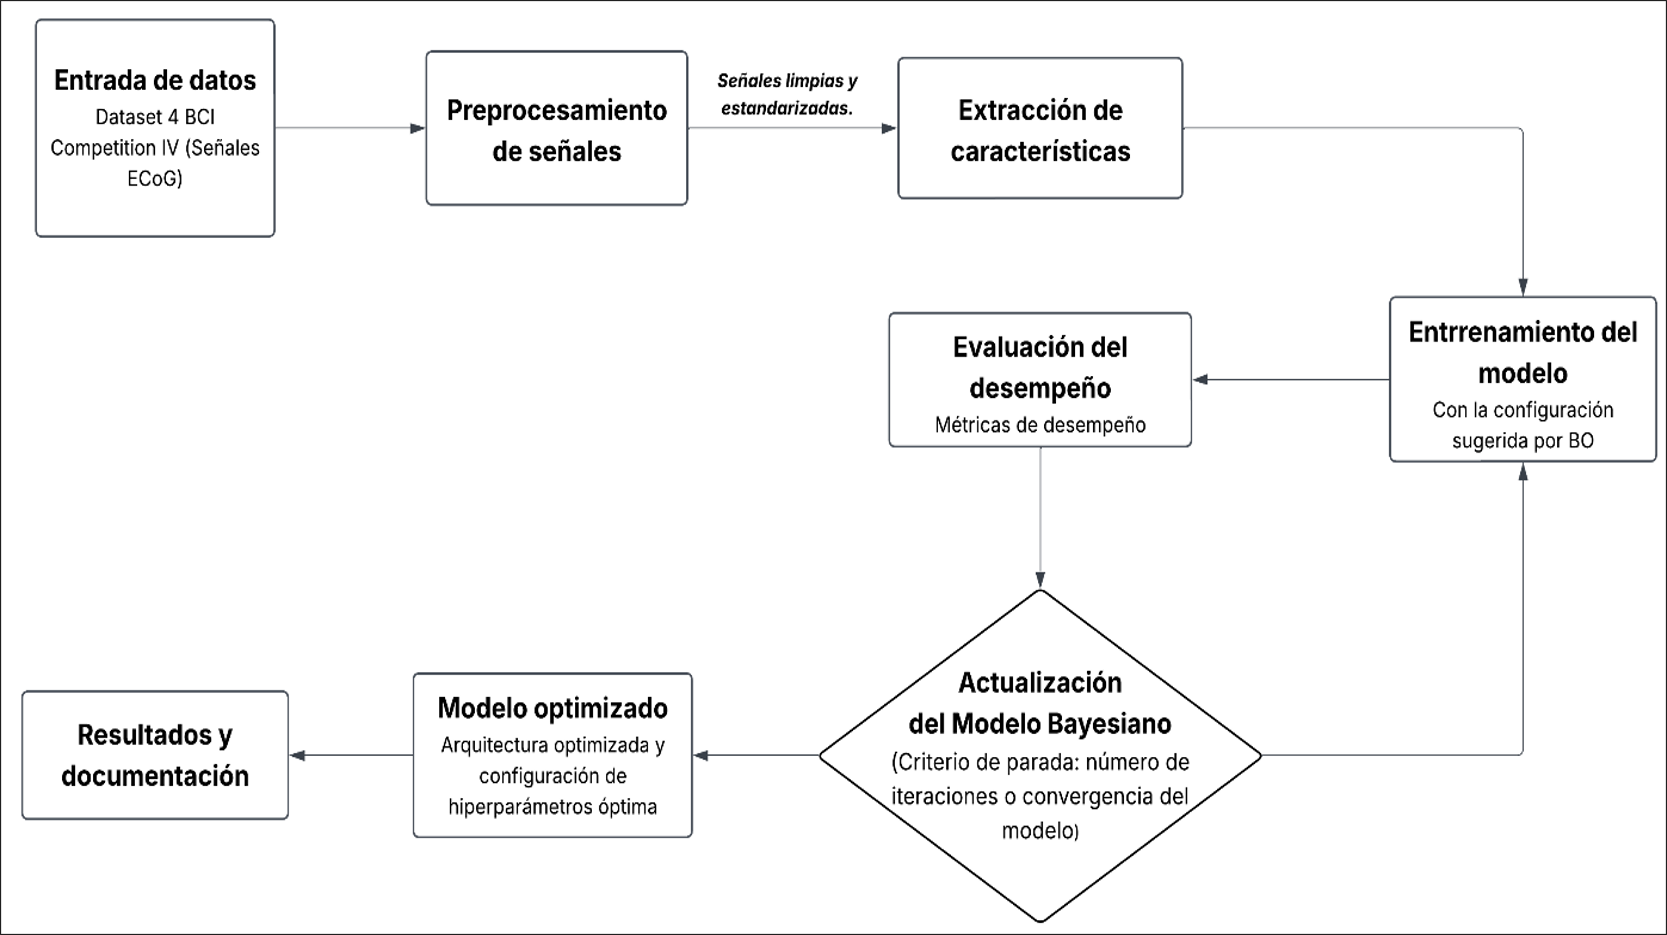
\includegraphics[width=\linewidth,height=0.44\textheight,keepaspectratio]{imgs/DiagramaProyecto.png}
      \figcap{A.1}{Flujo general del marco desarrollado desde la ingesta ECoG ($1000\text{ Hz}$) hasta la reconstrucci\'on continua de los 5 dedos ($100\text{ Hz}$). \textbf{Fuente:} Creaci\'on propia a partir de \cite{wirth2000crispdm} y el repositorio GitHub \cite{rodas_valencia_tpe_ecog}.}
    \end{column}
  \end{columns}

  \takeaway{El marco metodol\'ogico desacopla el preprocesamiento fijo (\texttt{P0}), el redise\~no arquitect\'onico (\texttt{A0}$\to$\texttt{A5}) y la optimizaci\'on bayesiana (\textbf{TPE}), permitiendo auditar el aporte de cada fase.}
\end{frame}

% --- ANEXO A2: EXCLUSIÓN DE CANALES CORRUPTOS ---
\begin{frame}{Anexo A2: Diagn\'ostico de Calidad y Exclusi\'on de Canales Corruptos}{Auditor\'ia f\'isica previa en TT1 para impedir la contaminaci\'on global de la rejilla cortical \cite{miller2008prediction,Schalk2011,rodas_valencia_tpe_ecog}}
  \begin{columns}[T,onlytextwidth]
    \begin{column}{0.48\textwidth}
      \centering
      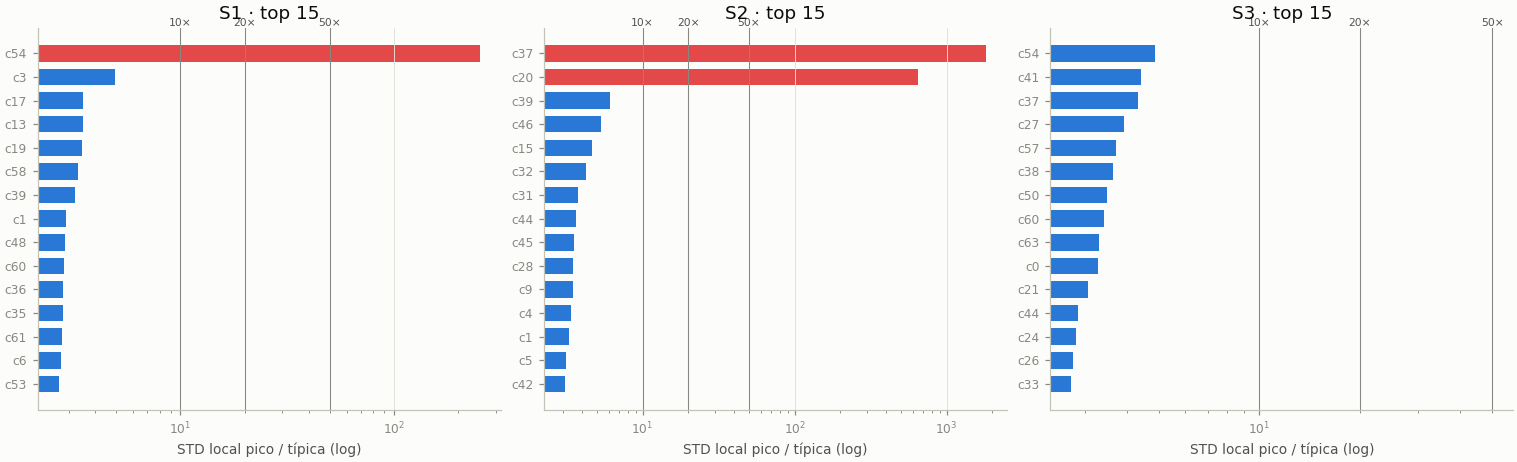
\includegraphics[width=\linewidth,height=0.46\textheight,keepaspectratio]{imgs/s02_ranking.png}
      \figcap{A.2}{Ranking de anomal\'ias de amplitud y varianza por electrodo en los tres sujetos (\texttt{S1}, \texttt{S2} y \texttt{S3}). \textbf{Fuente:} Obtenida del repositorio GitHub \cite{rodas_valencia_tpe_ecog}.}
    \end{column}
    \begin{column}{0.48\textwidth}
      \centering
      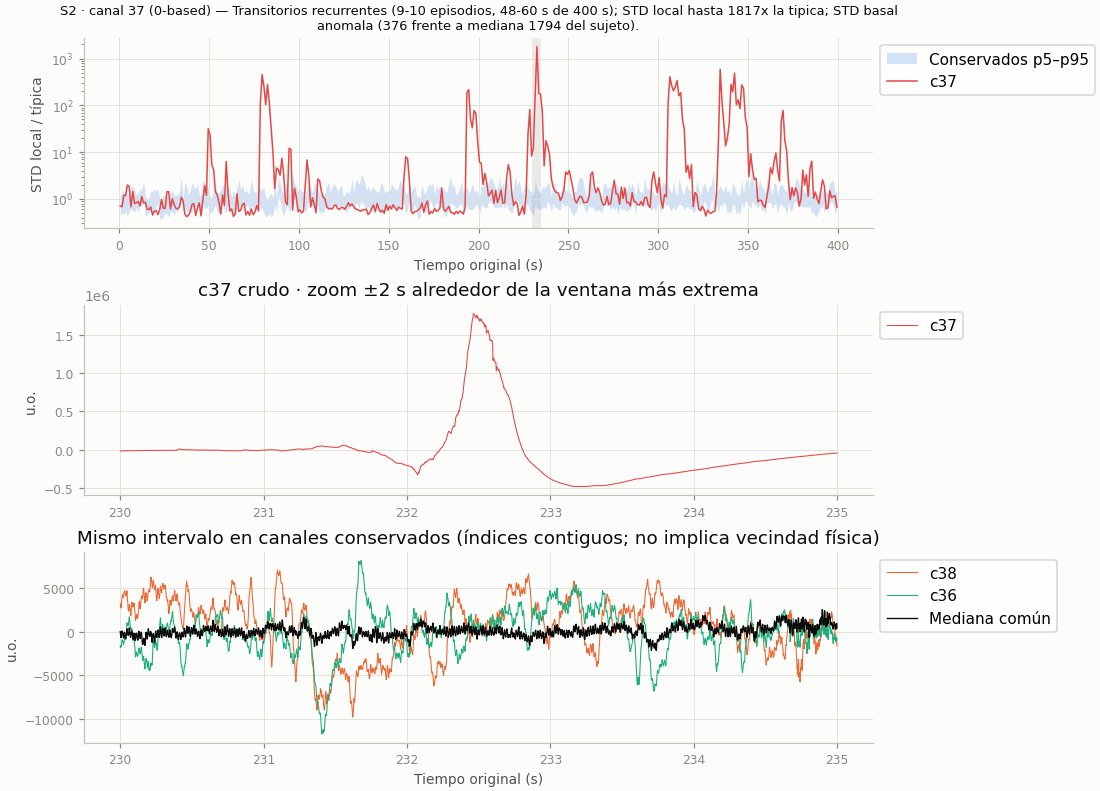
\includegraphics[width=\linewidth,height=0.46\textheight,keepaspectratio]{imgs/s02_S2_c037.png}
      \figcap{A.3}{Corrupci\'on instrumental severa en el canal \texttt{c037} del Sujeto 2 ($1817\times$ la desviaci\'on est\'andar basal). \textbf{Fuente:} Obtenida del repositorio GitHub \cite{rodas_valencia_tpe_ecog}.}
    \end{column}
  \end{columns}

  \takeaway{\textbf{Exclusi\'on fija previa:} \texttt{S1} excluye \texttt{c54} ($62\to 61$), \texttt{S2} excluye \texttt{c20} y \texttt{c37} ($48\to 46$), y \texttt{S3} excluye \texttt{c49} ($64\to 63$). Esto evita que un promedio com\'un inyecte pulsos de $>1800\sigma$ en los canales sanos antes de aplicar Referencia Mediana Com\'un (CMR) \cite{rodas_valencia_tpe_ecog}.}
\end{frame}

% --- ANEXO A3: EXTRACCIÓN DE CARACTERÍSTICAS HIGH-GAMMA ---
\begin{frame}{Anexo A3: Extracci\'on de Caracter\'isticas en la Banda High-Gamma}{Fundamento neurofisiol\'ogico de la banda $40\text{--}200\text{ Hz}$ abordado en TT1 \cite{kaplan2019decoding,Bundy2016,gruenwald2023highgamma}}
  \begin{columns}[c,onlytextwidth]
    \begin{column}{0.39\textwidth}
      \begin{block}{Biomarcadores Corticales en ECoG}
        \scriptsize
        \begin{itemize}\setlength{\itemsep}{3.5pt}
          \item \textbf{Bandas $\mu / \beta$ ($8\text{--}30\text{ Hz}$):} Exhiben desincronizaci\'on (ERD) difusa y no espec\'ifica al inicio del movimiento.
          \item \textbf{Banda High-Gamma ($40\text{--}200\text{ Hz}$):} Refleja el disparo poblacional neuronal local en la capa V de la corteza motora primaria (M1) \cite{Bundy2016,gruenwald2023highgamma}.
          \item \textbf{Selectividad somatot\'opica:} La potencia High-Gamma se correlaciona de forma directa y focalizada con la cinem\'atica individual de cada dedo \cite{kaplan2019decoding}.
        \end{itemize}
      \end{block}
    \end{column}

    \begin{column}{0.58\textwidth}
      \centering
      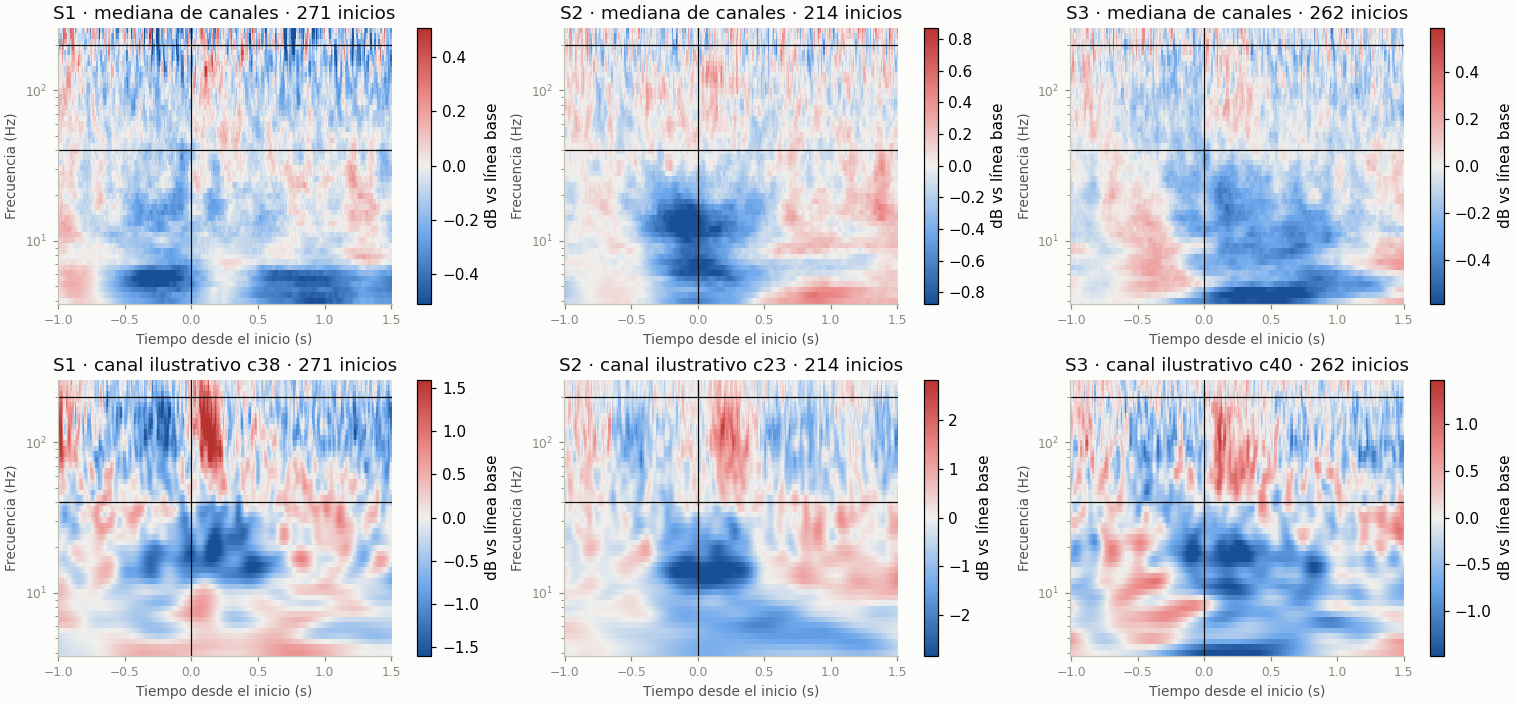
\includegraphics[width=\linewidth,height=0.52\textheight,keepaspectratio]{imgs/s04_ersp.png}
      \figcap{A.4}{Perturbaci\'on espectral ligada a eventos (ERSP) durante episodios de movimiento frente a reposo en la banda High-Gamma ($40\text{--}200\text{ Hz}$). \textbf{Fuente:} Obtenida del repositorio GitHub \cite{rodas_valencia_tpe_ecog}.}
    \end{column}
  \end{columns}

  \takeaway{La concentraci\'on de energ\'ia motora en la banda $40\text{--}200\text{ Hz}$ sustenta el uso de un banco denso de \textbf{40 ond\'iculas complejas de Morlet} para extraer la envolvente instant\'anea de potencia en cada electrodo \cite{kaplan2019decoding,rodas_valencia_tpe_ecog}.}
\end{frame}

% --- ANEXO A4: PIPELINE P0 Y COMPRESIÓN TEMPORAL DE DATOS ---
\begin{frame}{Anexo A4: Pipeline \texttt{P0} y Compresi\'on Temporal de Datos}{Acondicionamiento tiempo-frecuencia y reducci\'on de $1000\text{ Hz}$ a $100\text{ Hz}$ \cite{kaplan2019decoding,rodas_valencia_tpe_ecog}}
  \centering
  \begin{tikzpicture}[
    node distance=2.2mm,
    pbox/.style={rectangle, rounded corners=1.5mm, draw=ipnDark, fill=ipnSoft, thick, minimum height=9mm, inner sep=1.2mm, text width=1.82cm, align=center, font=\tiny\bfseries, text=textDark},
    arr/.style={-{Stealth[length=1.8mm]}, thick, ipnDark}
  ]
    \node[pbox] (b1) {1. Exclusi\'on y Clip\\$\pm 25\,\hat{\sigma}_{\text{MAD}}$};
    \node[pbox, right=of b1] (b2) {2. Referencia\\Mediana (CMR)};
    \node[pbox, right=of b2] (b3) {3. FIR Pasabanda\\y Notch Triple};
    \node[pbox, right=of b3] (b4) {4. CWT Morlet\\40 Bandas Log};
    \node[pbox, right=of b4] (b5) {5. Compresi\'on\\Kaiser $100\text{ Hz}$};
    \node[pbox, right=of b5, fill=rowHighlight] (b6) {6. Escalado Train\\Ventanas $W=256$};
    \draw[arr] (b1) -- (b2);
    \draw[arr] (b2) -- (b3);
    \draw[arr] (b3) -- (b4);
    \draw[arr] (b4) -- (b5);
    \draw[arr] (b5) -- (b6);
  \end{tikzpicture}

  \vspace{2mm}
  \begin{columns}[T,onlytextwidth]
    \begin{column}{0.48\textwidth}
      \begin{block}{Etapas 1 a 3: Limpieza y Filtrado Espectral}
        \scriptsize
        \begin{itemize}\setlength{\itemsep}{3pt}
          \item \textbf{Exclusi\'on fija + Clip MAD:} Canales v\'alidos ($\text{S1}:61, \text{S2}:46, \text{S3}:63$) y acotamiento $\pm 25\,\hat{\sigma}_{\text{MAD}}$.
          \item \textbf{Referencia Mediana Com\'un (CMR):} Sustracci\'on de la mediana espacial instant\'anea, inmune a valores at\'ipicos residuales.
          \item \textbf{Filtros FIR de fase cero:} Pasabanda en $\mathbf{40\text{--}200\text{ Hz}}$ ($331$ taps) y Notch en $\mathbf{60, 120, 180\text{ Hz}}$ ($1651$ taps).
        \end{itemize}
      \end{block}
    \end{column}

    \begin{column}{0.48\textwidth}
      \begin{block}{Etapas 4 a 6: Escalograma y Compresi\'on de Datos}
        \scriptsize
        \begin{itemize}\setlength{\itemsep}{3pt}
          \item \textbf{40 Wavelets de Morlet ($n_c=7$):} Potencia instant\'anea $P_{c,f_i}(t) = |(x_c * \psi_{f_i})(t)|^2$ en escala logar\'itmica.
          \item \textbf{Compresi\'on temporal ($10\times$) a $100\text{ Hz}$:} Decimaci\'on con filtro FIR Kaiser antialias ($243$ taps) y recorte de $\mathbf{\pm 125\text{ muestras}}$ de borde ($1250\text{ ms}$).
          \item \textbf{Escalado sin fuga:} \texttt{RobustScaler}$(10,90)$ en ECoG y \texttt{MinMaxScaler}$[0,1]$ en guante, ajustados \textbf{solo en train}.
        \end{itemize}
      \end{block}
    \end{column}
  \end{columns}
\end{frame}

% --- ANEXO A5: RECONSTRUCCIÓN DEL GUANTE Y ADELANTO TEMPORAL ---
\begin{frame}{Anexo A5: Reconstrucci\'on del Guante y Adelanto Temporal ($\tau = 20\text{ ms}$)}{Interpolaci\'on por Spline C\'ubico y compensaci\'on del desfase cortico-muscular \cite{miller2008prediction,rodas_valencia_tpe_ecog}}
  \begin{columns}[c,onlytextwidth]
    \begin{column}{0.39\textwidth}
      \begin{block}{Acondicionamiento de Etiquetas $y_d(t)$}
        \scriptsize
        \begin{itemize}\setlength{\itemsep}{3.5pt}
          \item \textbf{Problema del ZOH crudo:} El guante actualiza su lectura cada $40\text{ ms}$ ($25\text{ Hz}$), generando escalones artificiales con derivadas nulas y saltos discontinuos.
          \item \textbf{Interpolaci\'on Spline C\'ubico (\textit{Not-a-Knot}):} Se extraen los nodos reales ($n=40m$) y se reconstruye una curva suave con continuidad $C^2$ a $\mathbf{100\text{ Hz}}$.
          \item \textbf{Adelanto temporal ($\mathbf{\tau = 20\text{ ms}}$):} Desplazamiento de $+2\text{ muestras}$ a $100\text{ Hz}$ para compensar la latencia fisiol\'ogica entre la corteza motora y la flexi\'on mec\'anica del dedo.
        \end{itemize}
      \end{block}
    \end{column}

    \begin{column}{0.58\textwidth}
      \centering
      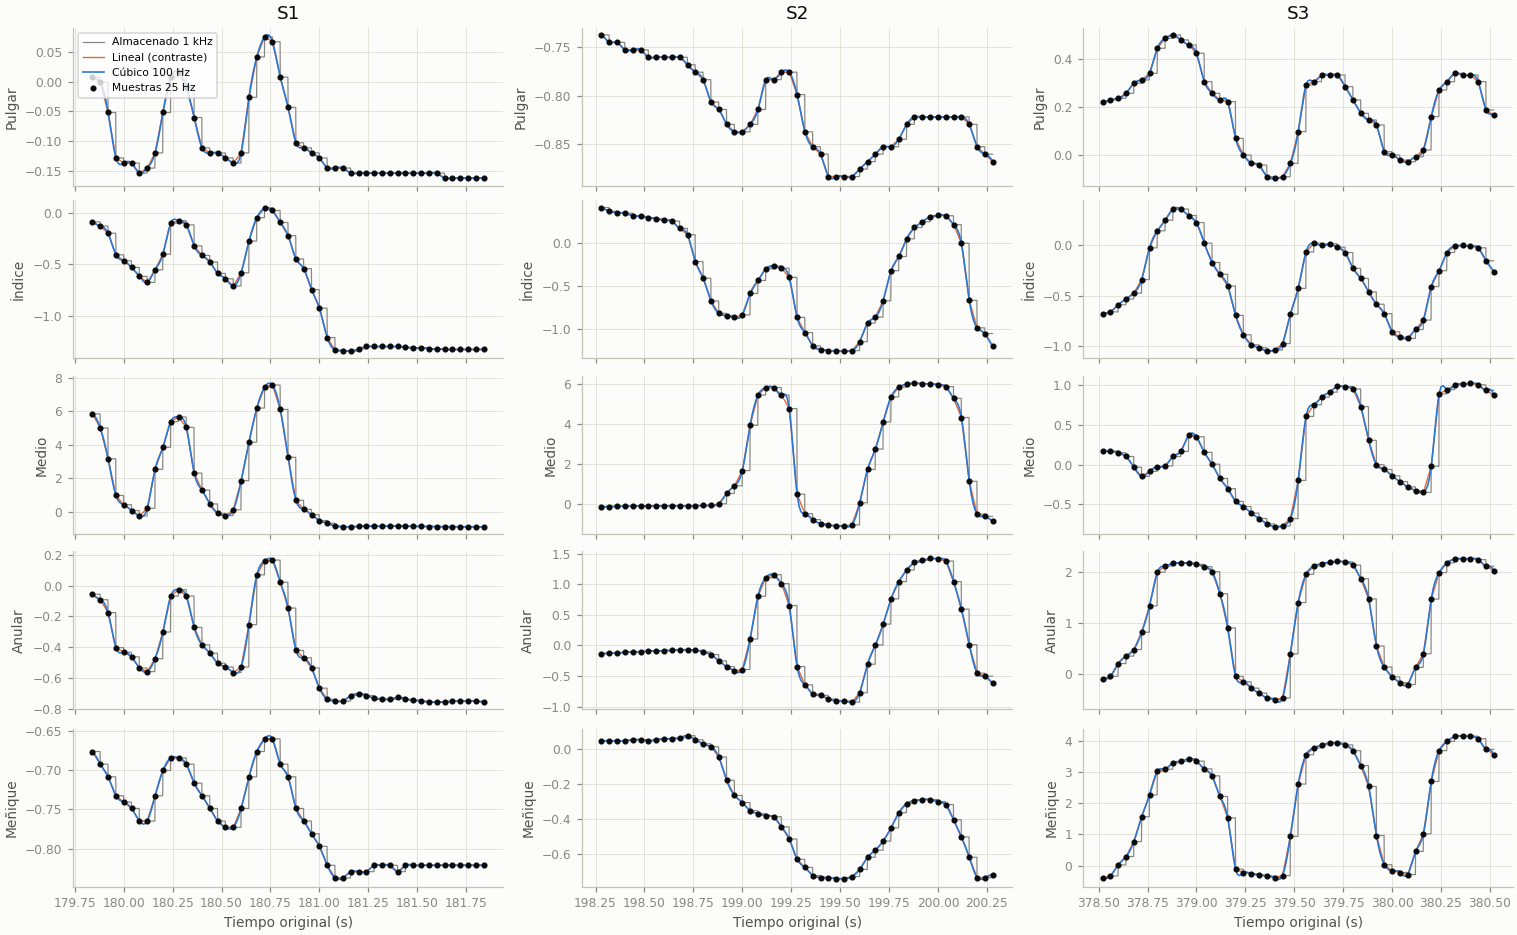
\includegraphics[width=\linewidth,height=0.48\textheight,keepaspectratio]{imgs/s08_glove_interpolation.png}
      \figcap{A.5}{Comparaci\'on entre la se\~nal escalonada original del guante (ZOH a $25\text{ Hz}$) y la trayectoria continua reconstruida mediante Spline C\'ubico a $100\text{ Hz}$. \textbf{Fuente:} Obtenida del repositorio GitHub \cite{rodas_valencia_tpe_ecog}.}
    \end{column}
  \end{columns}

  \takeaway{La interpolaci\'on por Spline C\'ubico elimina los artefactos de escal\'on del dataglove y permite entrenar la red neuronal con objetivos cinem\'aticos f\'isicamente diferenciables \cite{rodas_valencia_tpe_ecog}.}
\end{frame}

% --- ANEXO A6: DISEÑO DE LA ARQUITECTURA NEURONAL BASE A0 ---
\begin{frame}{Anexo A6: Dise\~no de la Arquitectura Base \texttt{A0} y Compresi\'on Espectral}{Topolog\'ia U-Net 1D (\texttt{EncoderDecoder1D}) desarrollada en TT1 \cite{ronneberger2015unet,Lomtev2022,rodas_valencia_tpe_ecog}}
  \centering
  \begin{tikzpicture}[
    node distance=3mm,
    ubox/.style={rectangle, rounded corners=1.5mm, draw=ipnDark, fill=ipnSoft, thick, minimum height=9mm, inner sep=1.2mm, text width=2.12cm, align=center, font=\tiny\bfseries, text=textDark},
    arr/.style={-{Stealth[length=2mm]}, thick, ipnDark}
  ]
    \node[ubox] (s1) {Entrada 2D\\$(C_{\text{v\'al}}\!\cdot\! 40) \times 256$};
    \node[ubox, right=of s1] (s2) {Bloque \textit{Stem}\\Compresi\'on $\to f$};
    \node[ubox, right=of s2] (s3) {Encoder 1D\\$L$ niveles ($d\in\{1,2,3\}$)};
    \node[ubox, right=of s3] (s4) {Decoder + \textit{Skips}\\Fusi\'on multiescala};
    \node[ubox, right=of s4, fill=rowHighlight] (s5) {Salida + OLA\\$5 \times 7750$ muestras};
    \draw[arr] (s1) -- (s2);
    \draw[arr] (s2) -- (s3);
    \draw[arr] (s3) -- (s4);
    \draw[arr] (s4) -- (s5);
    \draw[dashed, thick, ipnMed, -{Stealth[length=1.8mm]}] (s3.north) to[bend left=22] node[above, font=\tiny\bfseries, text=ipnMed] {Conexiones de salto (\textit{skip})} (s4.north);
  \end{tikzpicture}

  \vspace{2mm}
  \begin{columns}[T,onlytextwidth]
    \begin{column}{0.48\textwidth}
      \begin{block}{Compresi\'on Espectral y Codificador}
        \scriptsize
        \begin{itemize}\setlength{\itemsep}{3pt}
          \item \textbf{Compresi\'on espacial-espectral (\textit{Stem}):} Reduce la dimensi\'on de entrada ($2440, 1840\text{ o }2520$ canales tiempo-frecuencia) hacia $f \in \{64, 96\}$ mapas latentes.
          \item \textbf{Codificador con dilataci\'on:} $L \in \{4, 5\}$ niveles con multiplicadores $[1,2,4,8,8]\cdot f$, activaci\'on \texttt{GELU} y dilataci\'on $d \in \{1,2,3\}$ para ampliar el campo receptivo temporal.
        \end{itemize}
      \end{block}
    \end{column}

    \begin{column}{0.48\textwidth}
      \begin{block}{Decodificaci\'on y Reconstrucci\'on Continua}
        \scriptsize
        \begin{itemize}\setlength{\itemsep}{3pt}
          \item \textbf{Conexiones de salto (\textit{Skip Connections}):} Preservan la localizaci\'on temporal fina de las envolventes High-Gamma \cite{ronneberger2015unet}.
          \item \textbf{Reconstrucci\'on \textit{Overlap-Add} (OLA):} Las predicciones sobre $119$ ventanas deslizantes ($W=256$, paso $64$) se promedian para reconstruir los $N=7750$ instantes completos de cada bloque.
        \end{itemize}
      \end{block}
    \end{column}
  \end{columns}
\end{frame}

% 7. Anexos Adicionales de Defensa (Índice Extra y Anexos A7 a A20)
% =========================================================================
% MÓDULO 7: ANEXOS ADICIONALES DE DEFENSA PARA PREGUNTAS DEL JURADO (A7 A A20)
% =========================================================================

% --- ÍNDICE INTERACTIVO DE ANEXOS ADICIONALES ---
\begin{frame}{\'Indice de Anexos Adicionales para Preguntas del Jurado}{Respaldo t\'ecnico exhaustivo organizado por eje tem\'atico de defensa \cite{rodas_valencia_tpe_ecog}}
  \label{anexo:indice_extra}
  \vspace{-1.5mm}
  \begin{columns}[T,onlytextwidth]
    \begin{column}{0.49\textwidth}
      \begin{block}{1. Preprocesamiento y Filtrado Espectral}
        \tiny
        \begin{itemize}\setlength{\itemsep}{-0.5pt}
          \item \hyperlink{anexo:exclusion_canales}{\beamerbutton{Anexo A7}} Exclusi\'on fija de canales sin etiquetas (\texttt{c54, c20, c37, c49}).
          \item \hyperlink{anexo:cmr_notch}{\beamerbutton{Anexo A8}} Ecuaci\'on CMR vs.\ CAR y filtro FIR Notch ($1651$ taps).
          \item \hyperlink{anexo:ersp_antialias}{\beamerbutton{Anexo A9}} Justificaci\'on High-Gamma y decimaci\'on Antialias Kaiser.
          \item \hyperlink{anexo:ablacion_preproc}{\beamerbutton{Anexo A10}} Ablaciones secundarias de preprocesamiento (\texttt{P0, P1, P3, P5}).
        \end{itemize}
      \end{block}
      \vspace{-2.5mm}
      \begin{block}{2. Etiquetas, Auditor\'ia Antifuga y Ablaciones}
        \tiny
        \begin{itemize}\setlength{\itemsep}{-0.5pt}
          \item \hyperlink{anexo:zoh_overlap}{\beamerbutton{Anexo A11}} Desescalonado ZOH ($25\text{ Hz}$), purga $P=256$ y \textit{Overlap-Add}.
          \item \hyperlink{anexo:auditoria_v01_v14}{\beamerbutton{Anexo A12}} Huella SHA-256 y las 14 compuertas \texttt{V01--V14} (\texttt{pytest}).
          \item \hyperlink{anexo:ablaciones_detalle}{\beamerbutton{Anexo A13}} Desglose \texttt{A0}--\texttt{A5}/\texttt{A5b} y deltas apareados ($14/15$ folds).
        \end{itemize}
      \end{block}
    \end{column}

    \begin{column}{0.49\textwidth}
      \begin{block}{3. Par\'ametros, Checkpoint, TPE y Test Oficial}
        \tiny
        \begin{itemize}\setlength{\itemsep}{-0.5pt}
          \item \hyperlink{anexo:a5b_vs_a5_params}{\beamerbutton{Anexo A14}} Matem\'atica \texttt{A5b} vs.\ \texttt{A5} y conteo de par\'ametros ($9.35\text{--}28.03\text{ M}$).
          \item \hyperlink{anexo:checkpoint_retrospectivo}{\beamerbutton{Anexo A15}} Simulaci\'on retrospectiva de checkpoint ($0.6837 \to 0.7330$).
          \item \hyperlink{anexo:tpe_diagnostico}{\beamerbutton{Anexo A16}} Matem\'atica TPE ($\ell/g$), descomposici\'on de $+0.0672$ y 60 folds.
          \item \hyperlink{anexo:protocolos_test_brecha}{\beamerbutton{Anexo A17}} Protocolos de Test ($0.6333$ vs.\ $0.6669$) y brecha CV vs.\ Test.
        \end{itemize}
      \end{block}
      \vspace{-2.5mm}
      \begin{block}{4. Estado del Arte, Trazabilidad CSV y Poda}
        \tiny
        \begin{itemize}\setlength{\itemsep}{-0.5pt}
          \item \hyperlink{anexo:comparacion_dtcnet_dedos}{\beamerbutton{Anexo A18}} Comparaci\'on celda a celda ($15$ pares) \texttt{A5} vs.\ \textit{DTCNet} (2025).
          \item \hyperlink{anexo:trazabilidad_csv}{\beamerbutton{Anexo A19}} Matriz completa de 16 archivos CSV y 6 reglas de c\'alculo.
          \item \hyperlink{anexo:poda_y_privacidad}{\beamerbutton{Anexo A20}} Gobernanza de datos cl\'inicos y formulaci\'on de Poda Estructurada.
        \end{itemize}
      \end{block}
    \end{column}
  \end{columns}
\end{frame}

% --- ANEXO A7: EXCLUSIÓN FIJA DE CANALES DEFECTUOSOS ---
\begin{frame}{Anexo A7: Auditor\'ia de Calidad y Exclusi\'on Fija de Canales Defectuosos}{Pregunta del jurado: ?`Por qu\'e se excluyeron electrodos espec\'ificos y c\'omo garantizan que no usaron las etiquetas para elegirlos?}
  \label{anexo:exclusion_canales}
  \begin{columns}[T,onlytextwidth]
    \begin{column}{0.32\textwidth}
      \centering
      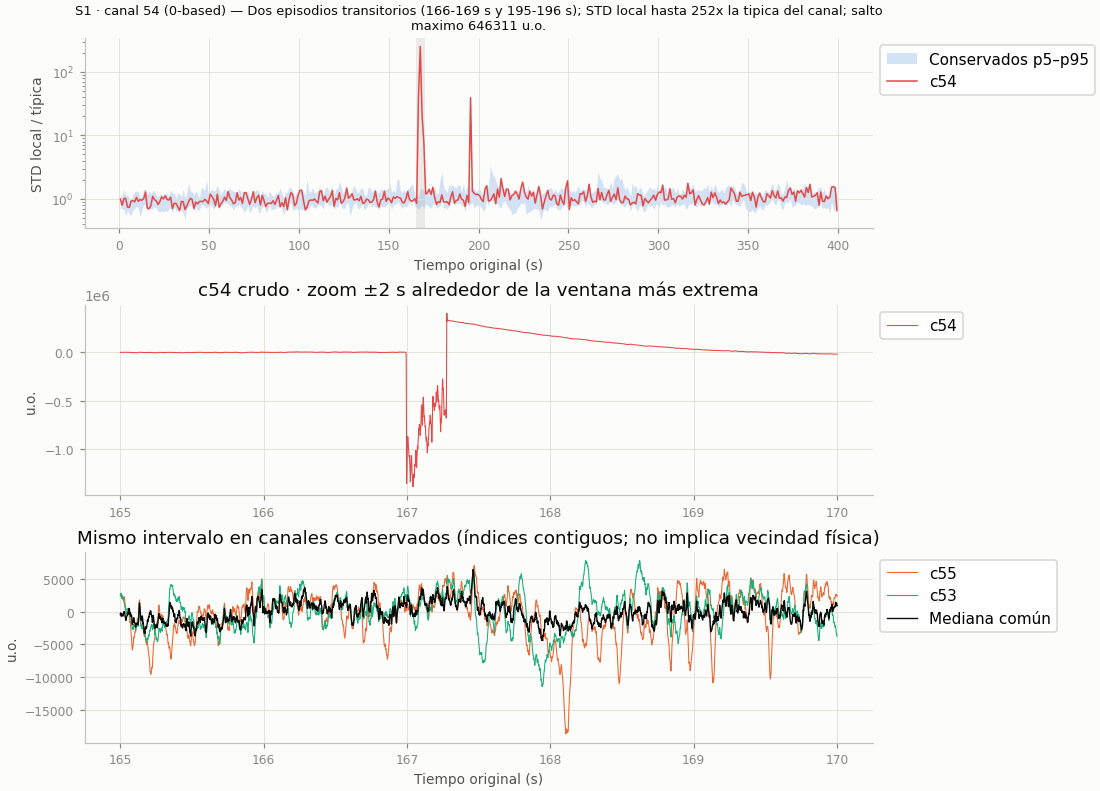
\includegraphics[width=\linewidth,height=0.36\textheight,keepaspectratio]{imgs/s02_S1_c054.png}
      \figcap{A.6}{Anomal\'ia en \texttt{S1-c054} ($62 \to 61$). \textbf{Fuente:} Obtenida de GitHub \cite{rodas_valencia_tpe_ecog}.}
    \end{column}
    \begin{column}{0.32\textwidth}
      \centering
      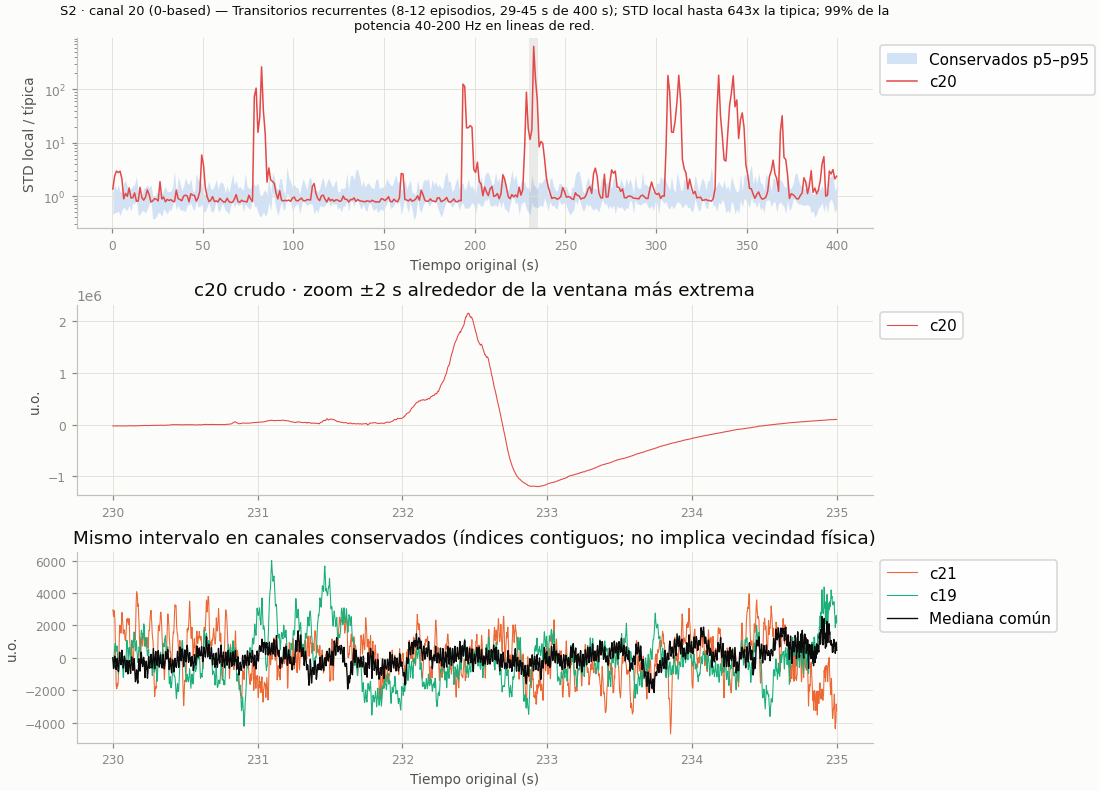
\includegraphics[width=\linewidth,height=0.36\textheight,keepaspectratio]{imgs/s02_S2_c020.png}
      \figcap{A.7}{Artefactos en \texttt{S2-c020} ($48 \to 46$). \textbf{Fuente:} Obtenida de GitHub \cite{rodas_valencia_tpe_ecog}.}
    \end{column}
    \begin{column}{0.32\textwidth}
      \centering
      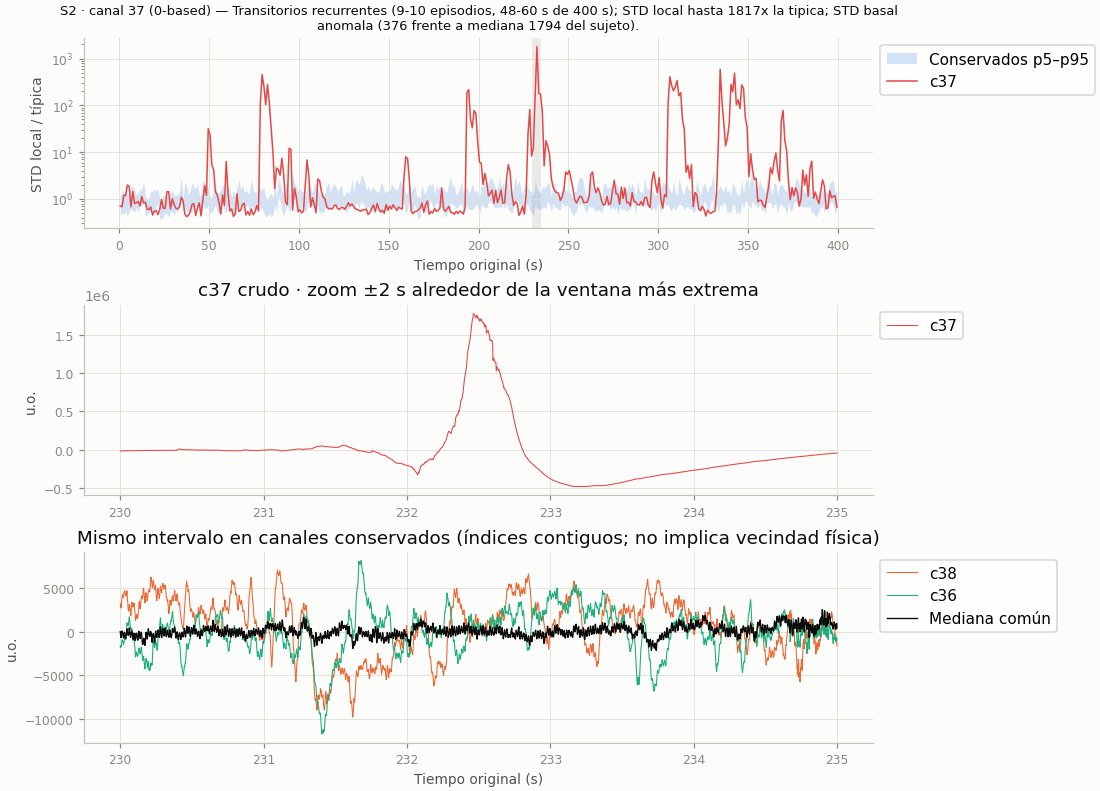
\includegraphics[width=\linewidth,height=0.36\textheight,keepaspectratio]{imgs/s02_S2_c037.png}
      \figcap{A.8}{Transitorio en \texttt{S2-c037} ($>1800\sigma$). \textbf{Fuente:} Obtenida de GitHub \cite{rodas_valencia_tpe_ecog}.}
    \end{column}
  \end{columns}

  \vspace{1mm}
  \begin{block}{Inspecci\'on Ciega a Etiquetas y Extirpaci\'on Previa a la Referencia Espacial}
    \scriptsize
    \begin{itemize}\setlength{\itemsep}{1.5pt}
      \item \textbf{Auditor\'ia exclusivamente sobre ECoG crudo de desarrollo:} La detecci\'on de saturaci\'on y varianza an\'omala se ejecut\'o sin consultar las trayectorias del guante (\texttt{dataglove}), bloqueando cualquier sesgo de selecci\'on de caracter\'isticas \cite{rodas_valencia_tpe_ecog}.
      \item \textbf{Canales extirpados antes de la CMR:} \texttt{S1}: canal $54$ ($62 \to 61$); \texttt{S2}: canales $20$ y $37$ ($48 \to 46$); \texttt{S3}: canal $49$ ($64 \to 63$). \hfill\hyperlink{anexo:indice_extra}{\beamerbutton{Volver al \'Indice Extra}}
    \end{itemize}
  \end{block}
\end{frame}

% --- ANEXO A8: CMR VS CAR Y FILTRADO FIR NOTCH ---
\begin{frame}{Anexo A8: Referencia Com\'un a la Mediana (CMR) vs.\ CAR y Filtrado FIR Notch}{Pregunta del jurado: ?`Por qu\'e usar CMR en lugar del promedio com\'un (CAR) y c\'omo se elimin\'o el ruido de l\'inea de $60\text{ Hz}$?}
  \label{anexo:cmr_notch}
  \begin{columns}[T,onlytextwidth]
    \begin{column}{0.48\textwidth}
      \centering
      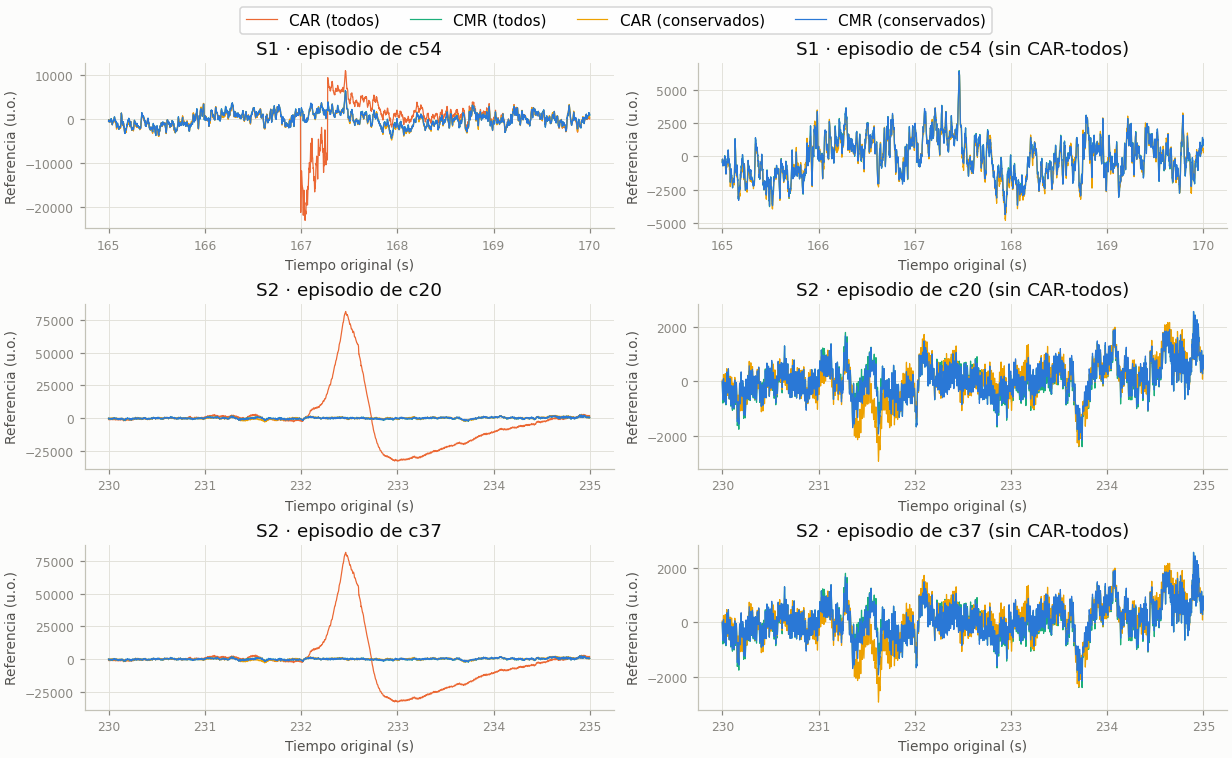
\includegraphics[width=\linewidth,height=0.37\textheight,keepaspectratio]{imgs/s03_reference_episodes.png}
      \figcap{A.9}{Inmunidad de CMR frente a contaminaci\'on global en CAR. \textbf{Fuente:} Obtenida de GitHub \cite{rodas_valencia_tpe_ecog}.}
    \end{column}
    \begin{column}{0.48\textwidth}
      \centering
      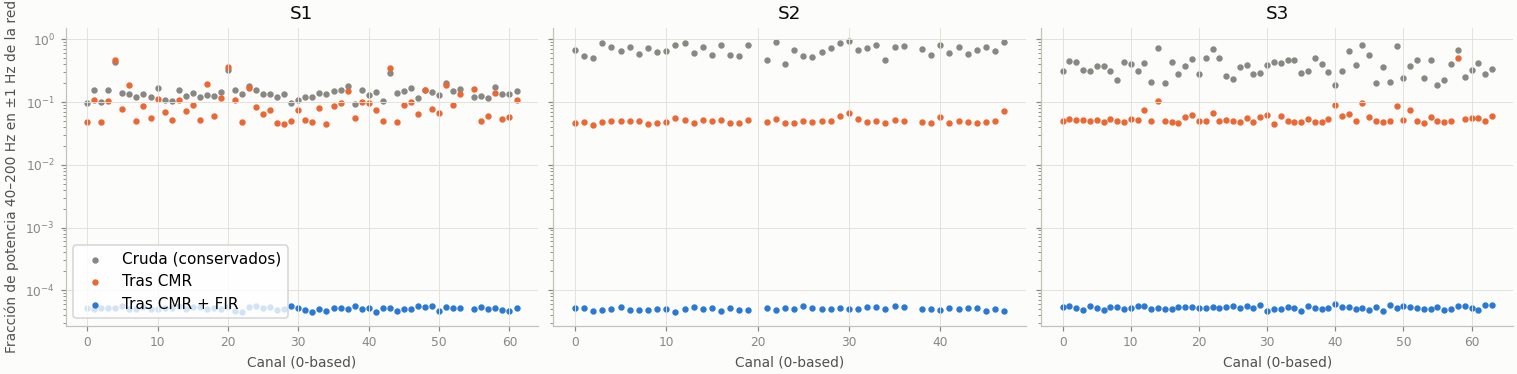
\includegraphics[width=\linewidth,height=0.37\textheight,keepaspectratio]{imgs/s05_line_fraction.png}
      \figcap{A.10}{Supresi\'on el\'ectrica en $60, 120, 180\text{ Hz}$ con Notch triple. \textbf{Fuente:} Obtenida de GitHub \cite{rodas_valencia_tpe_ecog}.}
    \end{column}
  \end{columns}

  \vspace{0.5mm}
  \begin{block}{Fundamento Matem\'atico de Robustez Espacial y Espectral}
    \scriptsize
    \begin{itemize}\setlength{\itemsep}{1.5pt}
      \item \textbf{Referencia Com\'un a la Mediana (CMR):} $\widetilde{X}_{c,t} = X_{c,t} - \operatorname{mediana}_{j \in C_{\text{v\'alidos}}}(X_{j,t})$. La mediana posee un \textbf{punto de ruptura del $50\%$} e impide que un artefacto local residual contamine a los canales sanos, a diferencia del promedio CAR \cite{Schalk2011,rodas_valencia_tpe_ecog}.
      \item \textbf{Filtro FIR Notch de fase cero ($1651$ taps):} Aten\'ua $>40\text{ dB}$ en $\mathbf{60, 120\text{ y }180\text{ Hz}}$ sin distorsi\'on de fase. \hfill\hyperlink{anexo:indice_extra}{\beamerbutton{Volver al \'Indice Extra}}
    \end{itemize}
  \end{block}
\end{frame}

% --- ANEXO A9: JUSTIFICACIÓN HIGH-GAMMA Y DECIMACIÓN ANTIALIAS KAISER ---
\begin{frame}{Anexo A9: Justificaci\'on High-Gamma ($40\text{--}200\text{ Hz}$) y Decimaci\'on Antialias Kaiser}{Pregunta del jurado: ?`Por qu\'e acotar las wavelets de Morlet a $40\text{--}200\text{ Hz}$ y c\'omo evitaron el aliasing al bajar de $1000\text{ Hz}$ a $100\text{ Hz}$?}
  \label{anexo:ersp_antialias}
  \begin{columns}[T,onlytextwidth]
    \begin{column}{0.48\textwidth}
      \centering
      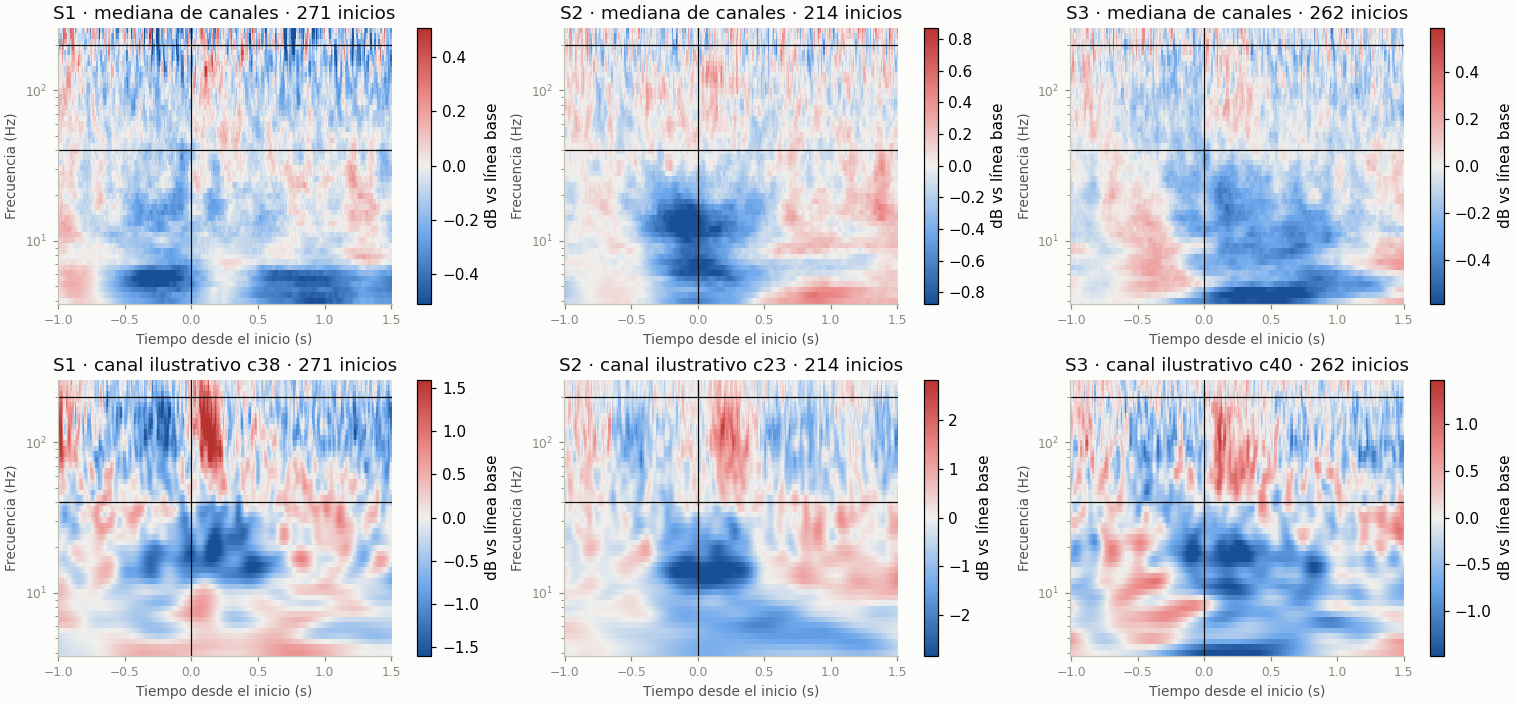
\includegraphics[width=\linewidth,height=0.37\textheight,keepaspectratio]{imgs/s04_ersp.png}
      \figcap{A.11}{Actividad motora acoplada en banda High-Gamma ($40\text{--}200\text{ Hz}$). \textbf{Fuente:} Obtenida de GitHub \cite{rodas_valencia_tpe_ecog}.}
    \end{column}
    \begin{column}{0.48\textwidth}
      \centering
      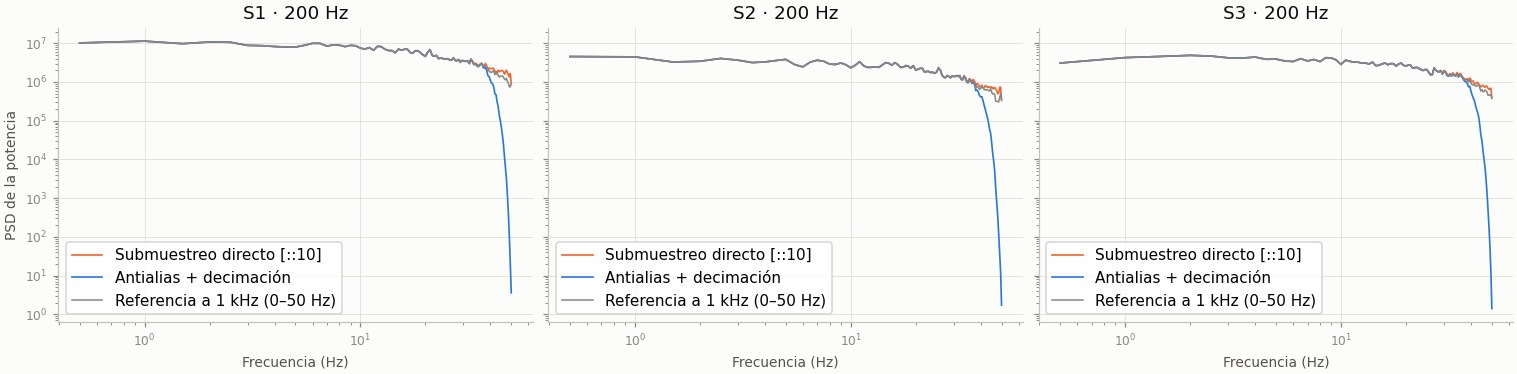
\includegraphics[width=\linewidth,height=0.37\textheight,keepaspectratio]{imgs/s07_naive_vs_antialias.png}
      \figcap{A.12}{Decimaci\'on FIR Kaiser ($243$ taps, $-60\text{ dB}$). \textbf{Fuente:} Obtenida de GitHub \cite{rodas_valencia_tpe_ecog}.}
    \end{column}
  \end{columns}

  \vspace{0.5mm}
  \begin{block}{Acoplamiento Tiempo-Frecuencia y Prevenci\'on del Plegado Espectral (\textit{Aliasing})}
    \scriptsize
    \begin{itemize}\setlength{\itemsep}{1.5pt}
      \item \textbf{Banco CWT de Morlet ($40$ escalas logar\'itmicas, $n_c=7$ ciclos):} Captura la envolvente de potencia sin\'aptica local en $40\text{--}200\text{ Hz}$ \cite{kaplan2019decoding,Bundy2016}.
      \item \textbf{Decimaci\'on Antialias ($1000\text{ Hz} \to 100\text{ Hz}$, Nyquist $=50\text{ Hz}$):} El filtro FIR con ventana de Kaiser ($243$ taps, rechazo de $-60\text{ dB}$) elimina fluctuaciones r\'apidas antes de diezmar por factor $10$, evitando el plegado espectral sobre la envolvente \cite{rodas_valencia_tpe_ecog}. \hfill\hyperlink{anexo:indice_extra}{\beamerbutton{Volver al \'Indice Extra}}
    \end{itemize}
  \end{block}
\end{frame}

% --- ANEXO A10: ABLACIONES SECUNDARIAS DE PREPROCESAMIENTO ---
\begin{frame}{Anexo A10: Ablaciones Secundarias de Preprocesamiento (\texttt{P0}, \texttt{P1}, \texttt{P3}, \texttt{P5})}{Pregunta del jurado: ?`Qu\'e ocurri\'o cuando probaron variantes del preprocesamiento sobre la red base \texttt{A0}?}
  \label{anexo:ablacion_preproc}
  \centering
  \resizebox{\textwidth}{!}{%
    \renewcommand{\arraystretch}{1.18}
    \begin{tabular}{>{\bfseries}l l c c c c c}
      \toprule
      \rowcolor{ipnDark}
      \textcolor{white}{Variante} & \textcolor{white}{Descripci\'on del cambio en el pipeline (sobre red base \texttt{A0}, \'epoca 50)} & \textcolor{white}{\texttt{S1}} & \textcolor{white}{\texttt{S2}} & \textcolor{white}{\texttt{S3}} & \textcolor{white}{Media CV ($r$)} & \textcolor{white}{$\Delta r$ vs.\ \texttt{P0}} \\
      \midrule
      \texttt{P0} (Fijado) & Pipeline de referencia fijado (Exclusi\'on + CMR + FIR + 40 Morlet + Kaiser) & $0.4990$ & $0.4289$ & $0.7187$ & $0.5489$ & --- \\
      \rowcolor{rowHighlight}
      \texttt{P1} & Sin referencia espacial CMR (conservando el resto de \texttt{P0} id\'entico) & $0.4992$ & $\mathbf{0.5446}$ & $0.7220$ & $\mathbf{0.5886}$ & $\mathbf{+0.0397}$ \\
      \texttt{P3} & Variante espectral secundaria evaluada en Secci\'on 3.6 & --- & --- & --- & $0.5572$ & $+0.0084$ \\
      \rowcolor{rowLight}
      \texttt{P5} & Variante de acondicionamiento secundaria evaluada en Secci\'on 3.6 & --- & --- & --- & $0.5498$ & $+0.0009$ \\
      \bottomrule
    \end{tabular}%
  }
  \fuente{Creaci\'on propia, obtenida del repositorio GitHub \cite{rodas_valencia_tpe_ecog}.}

  \vspace{1.5mm}
  \begin{block}{Lectura Metodol\'ogica Rigurosa (Secci\'on 3.6 del Reporte Experimental)}
    \scriptsize
    \begin{itemize}\setlength{\itemsep}{2.5pt}
      \item \textbf{Origen de la diferencia en \texttt{P1}:} Al evaluar \texttt{P1} (sin CMR) sobre la arquitectura inicial \texttt{A0} en la \'epoca 50, la media subi\'o a $\mathbf{0.5886}$ ($\Delta = +0.0397$), concentrada casi por completo en el \textbf{Sujeto 2 ($\mathbf{+0.1157}$)}.
      \item \textbf{Por qu\'e \texttt{P0} se mantuvo fijo:} La b\'usqueda bayesiana \textbf{TPE} y las ablaciones \texttt{A1}--\texttt{A5} se ejecutaron con \texttt{P0} congelado para garantizar comparabilidad estricta; \texttt{P1} no fue evaluado de forma controlada con la arquitectura final \texttt{A5} optimizada.
      \item \textbf{Interpretaci\'on honesta:} Por ello, \texttt{P0} se documenta como el \textbf{pipeline de referencia fijado para la comparabilidad experimental}, y no como el mejor preprocesamiento posible demostrado \cite{rodas_valencia_tpe_ecog}. \hfill\hyperlink{anexo:indice_extra}{\beamerbutton{Volver al \'Indice Extra}}
    \end{itemize}
  \end{block}
\end{frame}

% --- ANEXO A11: DESESCALONADO ZOH, PURGA Y OVERLAP-ADD ---
\begin{frame}{Anexo A11: Desescalonado ZOH ($25\text{ Hz}$), Purga ($P=256$) y \textit{Overlap-Add}}{Pregunta del jurado: ?`C\'omo se corrigi\'o el escalonado del guante y c\'omo se reconstruye la trayectoria continua para medir Pearson?}
  \label{anexo:zoh_overlap}
  \begin{columns}[c,onlytextwidth]
    \begin{column}{0.48\textwidth}
      \begin{block}{1. Desescalonado ZOH y Purga Antifuga}
        \scriptsize
        \begin{itemize}\setlength{\itemsep}{2pt}
          \item \textbf{Almacenamiento ZOH:} El guante muestrea a $25\text{ Hz}$ pero se repite cada $40$ muestras a $1000\text{ Hz}$: $\texttt{train\_dg}[n] = g_{\text{real}}[\lfloor n/40 \rfloor]$.
          \item \textbf{Spline + Adelanto:} Se extraen las muestras reales ($n=40m$), se interpola con Spline C\'ubico \textit{Not-a-Knot} a $100\text{ Hz}$ y se adelanta $\tau = 20\text{ ms}$ ($+2$ muestras).
          \item \textbf{Bordes y Purga:} Recorte de $\pm 125$ muestras por bloque ($N=7750$ v\'alidas) y purga de $\mathbf{P=256\text{ muestras}}$ en fronteras de train adyacentes a validaci\'on.
        \end{itemize}
      \end{block}

      \begin{block}{2. Reconstrucci\'on \textit{Overlap-Add} ($119$ Ventanas)}
        \scriptsize
        Se deslizan $118$ ventanas ($W=256, s=64$) m\'as la ventana $\#119$ anclada en $[7494, 7750)$, promediando $\widehat{Y}_d[k] = S_d[k]/C[k]$ antes de medir Pearson sobre la trayectoria completa.
      \end{block}
    \end{column}

    \begin{column}{0.49\textwidth}
      \centering
      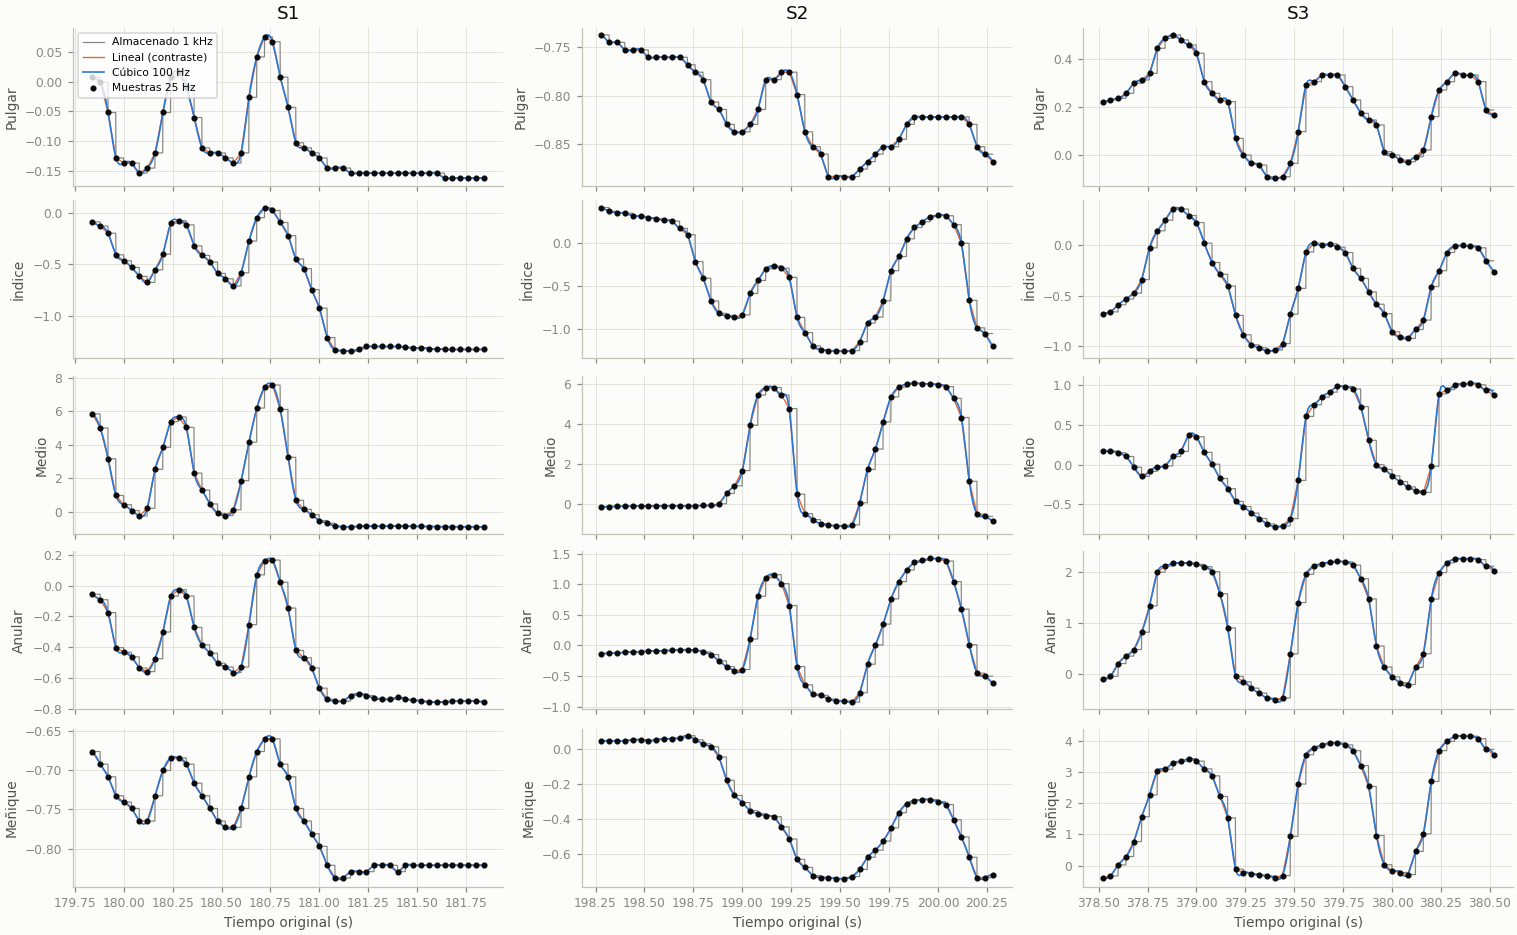
\includegraphics[width=\linewidth,height=0.45\textheight,keepaspectratio]{imgs/s08_glove_interpolation.png}
      \figcap{A.13}{Eliminaci\'on de escalones ZOH ($25\text{ Hz}$) mediante Spline C\'ubico a $100\text{ Hz}$. \textbf{Fuente:} Obtenida del repositorio GitHub \cite{rodas_valencia_tpe_ecog}.}
      \vspace{1mm}
      \hfill\hyperlink{anexo:indice_extra}{\beamerbutton{Volver al \'Indice Extra}}
    \end{column}
  \end{columns}
\end{frame}

% --- ANEXO A12: HUELLA SHA-256 Y COMPUERTAS V01-V14 ---
\begin{frame}{Anexo A12: Huella Criptogr\'afica SHA-256 y las 14 Compuertas (\texttt{V01--V14})}{Pregunta del jurado: ?`Qu\'e pruebas de software certifican que no existi\'o fuga de datos (\textit{data leakage}) entre bloques?}
  \label{anexo:auditoria_v01_v14}
  \centering
  \scriptsize
  \renewcommand{\arraystretch}{1.18}
  \begin{tabularx}{\textwidth}{>{\bfseries\color{ipnDark}}l l >{\raggedright\arraybackslash}X}
    \toprule
    \rowcolor{ipnDark}
    \textcolor{white}{Bloque} & \textcolor{white}{Compuertas \texttt{pytest}} & \textcolor{white}{Verificaci\'on automatizada y garant\'ia metodol\'ogica certificada} \\
    \midrule
    \texttt{V01--V03} & Integridad de origen y canales & Inmutabilidad de archivos \texttt{.mat} crudos, bloqueo estricto de \texttt{test\_labels} durante desarrollo y exclusi\'on fija de canales corruptos previa al c\'alculo de la mediana espacial CMR. \\
    \rowcolor{rowLight}
    \texttt{V04--V06} & Partici\'on, escalado y latencia & Separaci\'on cronol\'ogica con purga $P=256$, ajuste de \texttt{RobustScaler}$(10,90)$ y \texttt{MinMaxScaler}$[0,1]$ exclusivamente sobre train, y alineaci\'on temporal $\tau=20\text{ ms}$. \\
    \rowcolor{rowHighlight}
    \texttt{V07--V08} & \textbf{Experimento contrafactual bit a bit} & Se inyecta un impulso gigante ($\mathbf{10^6 \times \max|\text{ECoG}|}$) en el bloque de validaci\'on crudo; al regenerar el fold, los tensores v\'alidos de entrenamiento permanecen \textbf{id\'enticos bit a bit ($\text{tolerancia} = 0.0$)}. \\
    \texttt{V09--V14} & Soporte DSP, OLA y m\'etricas & Verificaci\'on de bordes FIR/Morlet ($\pm 125$ muestras), conteo exacto de $119$ ventanas, cobertura $C[k]\ge 1$ en \textit{overlap-add}, validez de \texttt{A0--A5} y f\'ormulas de $r$, $\operatorname{CCC}$ y $\operatorname{MSE}$. \\
    \bottomrule
  \end{tabularx}
  \fuente{Creaci\'on propia, obtenida del repositorio GitHub \cite{rodas_valencia_tpe_ecog}.}

  \vspace{2mm}
  \begin{block}{Identificador Inmutable \texttt{pipeline\_id} (SHA-256)}
    \scriptsize
    Cada artefacto preprocesado registra un hash criptogr\'afico \textbf{SHA-256} derivado de los hiperpar\'ametros de filtrado, escalado y partici\'on, impidiendo mezclar tensores de distintas configuraciones \cite{rodas_valencia_tpe_ecog}. \hfill\hyperlink{anexo:indice_extra}{\beamerbutton{Volver al \'Indice Extra}}
  \end{block}
\end{frame}

% --- ANEXO A13: DESGLOSE COMPLETO DE ABLACIONES ARQUITECTÓNICAS ---
\begin{frame}{Anexo A13: Desglose de Ablaciones Arquitect\'onicas (\texttt{A0}--\texttt{A5}, \texttt{A5b}) y Deltas}{Pregunta del jurado: ?`Por qu\'e no se puede afirmar que \texttt{ConvTranspose1d} mejora el rendimiento por s\'i sola?}
  \label{anexo:ablaciones_detalle}
  \begin{columns}[c,onlytextwidth]
    \begin{column}{0.48\textwidth}
      \centering
      \resizebox{\linewidth}{!}{%
        \renewcommand{\arraystretch}{1.16}
        \begin{tabular}{>{\bfseries}l l c c}
          \toprule
          \rowcolor{ipnDark}
          \textcolor{white}{Red} & \textcolor{white}{Configuraci\'on (\'epoca 50 fija)} & \textcolor{white}{Media CV} & \textcolor{white}{$\Delta r$ vs.\ \texttt{A0}} \\
          \midrule
          \texttt{A0/P0} & Base U-Net 1D (\texttt{BatchNorm1d}) & $0.5489$ & --- \\
          \rowcolor{rowLight}
          \texttt{A1} & + \texttt{LayerNorm} por grupo temporal & $0.6094$ & $+0.0605$ \\
          \texttt{A2} & + \texttt{Dropout} espacial $p=0.10$ & $0.6219$ & $+0.0731$ \\
          \rowcolor{ipnSoft}
          \texttt{A3} & + \texttt{ConvTranspose1d} aislada & $\mathbf{0.5173}$ & $\mathbf{-0.0316}$ \\
          \texttt{A4} & + \textit{Skip} previo a \texttt{Conv1d} & $0.5806$ & $+0.0317$ \\
          \rowcolor{rowLight}
          \texttt{A5b} & Combinada (\texttt{A1+A2+A4}) con interp. & $0.6779$ & $+0.1291$ \\
          \rowcolor{rowHighlight}
          \texttt{A5} & Combinada + \texttt{ConvTranspose} \textit{depthwise} & $\mathbf{0.6837}$ & $\mathbf{+0.1349}$ \\
          \bottomrule
        \end{tabular}%
      }
      \fuente{Creaci\'on propia, obtenida del repositorio GitHub \cite{rodas_valencia_tpe_ecog}.}

      \vspace{1.5mm}
      \begin{block}{Deltas Apareados $\texttt{A0} \to \texttt{A5}$ ($14/15$ Folds $+$) }
        \tiny
        \texttt{S1}: $+0.1048$ ($4/5$ folds; \'unica excepci\'on \texttt{S1-B3} con $-0.0359$).\\
        \texttt{S2}: $\mathbf{+0.1927}$ ($5/5$ folds) \,|\, \texttt{S3}: $\mathbf{+0.1070}$ ($5/5$ folds).
      \end{block}
    \end{column}

    \begin{column}{0.49\textwidth}
      \centering
      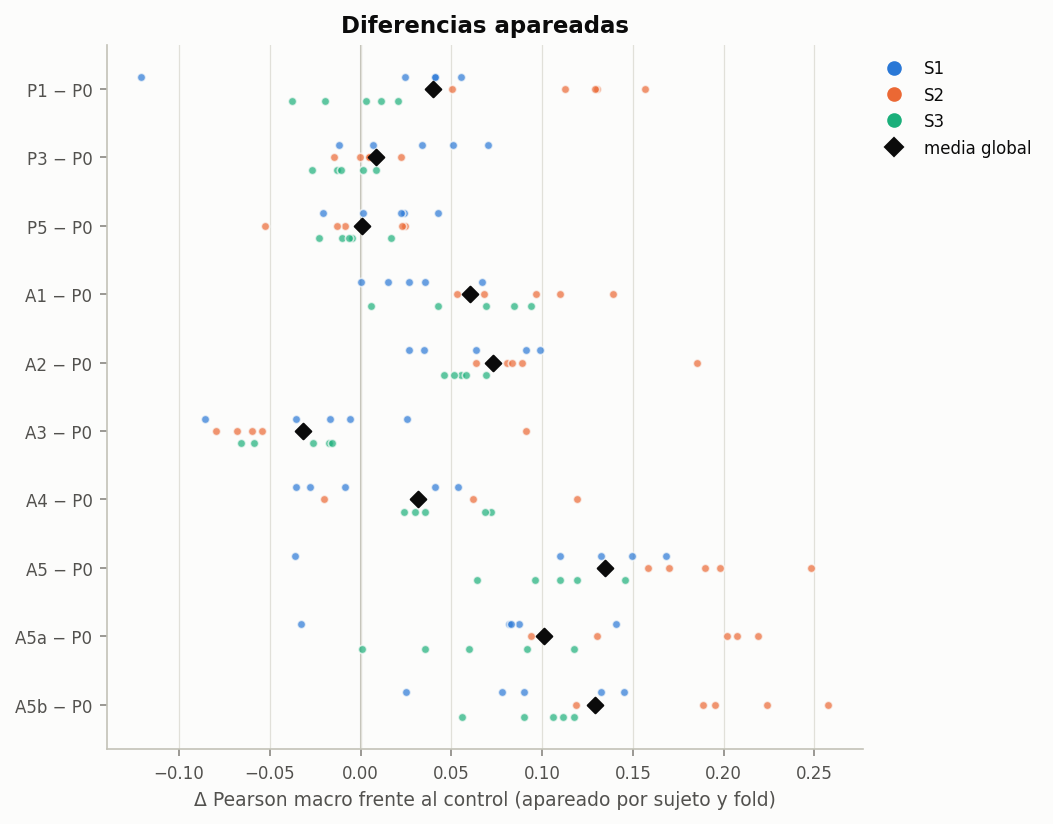
\includegraphics[width=0.48\linewidth,height=0.36\textheight,keepaspectratio]{imgs/paired_deltas.png}\hfill
      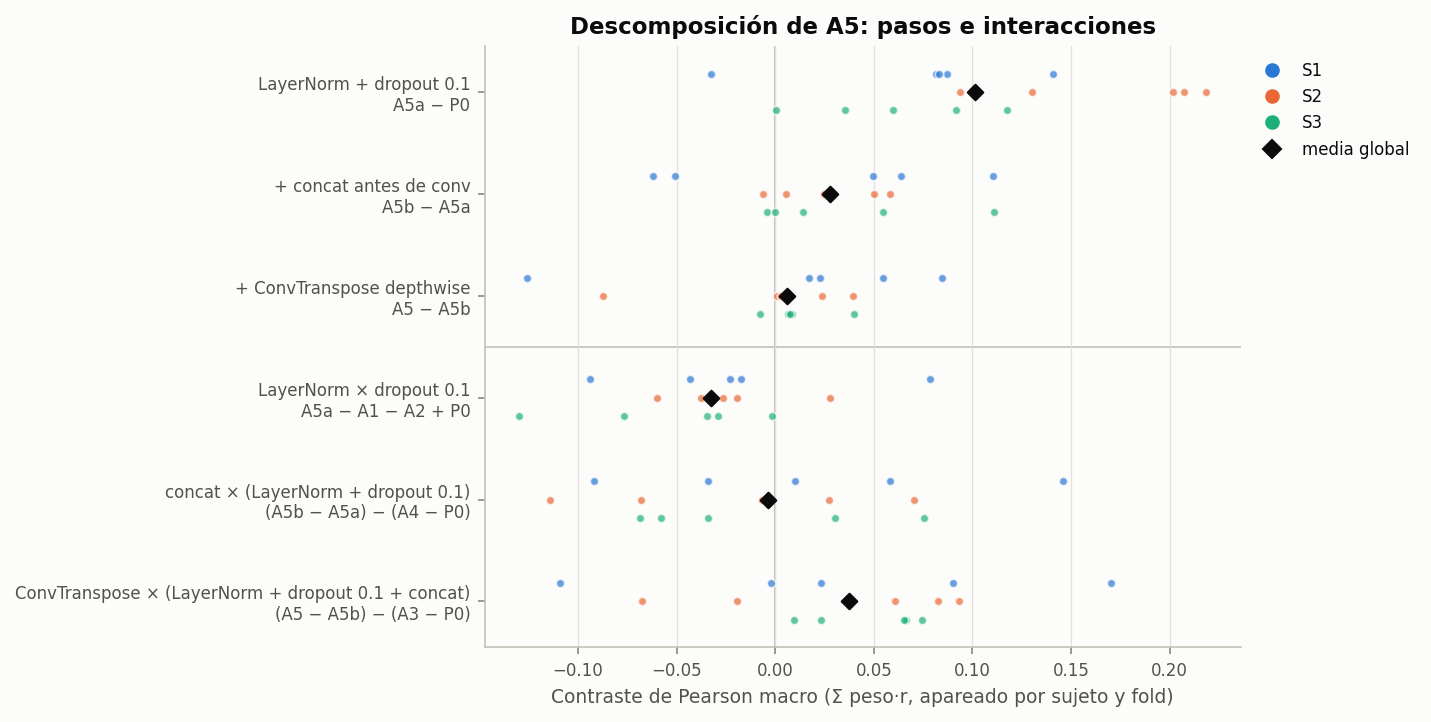
\includegraphics[width=0.48\linewidth,height=0.36\textheight,keepaspectratio]{imgs/contrasts.png}
      \figcap{A.14}{Izquierda: deltas apareados por pliegue ($\texttt{A0}\to\texttt{A5}$). Derecha: contrastes de efectos individuales y sin\'ergicos. \textbf{Fuente:} Obtenida del repositorio GitHub \cite{rodas_valencia_tpe_ecog}.}
      \vspace{1mm}
      \hfill\hyperlink{anexo:indice_extra}{\beamerbutton{Volver al \'Indice Extra}}
    \end{column}
  \end{columns}
\end{frame}

% --- ANEXO A14: MATEMÁTICA A5B VS A5 Y CONTEO DE PARÁMETROS ---
\begin{frame}{Anexo A14: Matem\'atica \texttt{A5b} vs.\ \texttt{A5} y Conteo de Par\'ametros por Sujeto}{Pregunta del jurado: ?`Cu\'al es la diferencia matem\'atica entre el decoder de \texttt{A5b} y \texttt{A5}, y cu\'antos par\'ametros tiene cada red?}
  \label{anexo:a5b_vs_a5_params}
  \begin{columns}[T,onlytextwidth]
    \begin{column}{0.48\textwidth}
      \begin{block}{1. Interpolaci\'on (\texttt{A5b}) vs.\ \texttt{ConvTranspose1d} (\texttt{A5})}
        \scriptsize
        \begin{itemize}\setlength{\itemsep}{3pt}
          \item \textbf{Variante \texttt{A5b} ($0$ par\'ametros en sobremuestreo):} Emplea interpolaci\'on lineal vectorizada con pesos geom\'etricos fijos ($0.75$ y $0.25$) para duplicar la resoluci\'on temporal en cada nivel del decodificador.
          \item \textbf{Variante \texttt{A5} (\texttt{ConvTranspose1d} \textit{depthwise}):} Configura $k=4, s=2, p=1, \text{groups}=C$, a\~nadiendo solo $\mathbf{4C\text{ pesos por nivel}}$. Incluye a la interpolaci\'on lineal como caso particular exacto y aprende el perfil de reconstrucci\'on temporal por canal \cite{rodas_valencia_tpe_ecog}.
        \end{itemize}
      \end{block}
    \end{column}

    \begin{column}{0.49\textwidth}
      \begin{block}{2. Conteo de Par\'ametros Ganadores (\texttt{tpe\_trials.csv})}
        \centering
        \resizebox{\linewidth}{!}{%
          \renewcommand{\arraystretch}{1.18}
          \begin{tabular}{>{\bfseries}l c c c r}
            \toprule
            \rowcolor{ipnDark}
            \textcolor{white}{Sujeto} & \textcolor{white}{Trial} & \textcolor{white}{Topolog\'ia ($k, L, f$)} & \textcolor{white}{Canales ECoG} & \textcolor{white}{Par\'ametros} \\
            \midrule
            \texttt{S1} & $\#10$ & $k=5, L=5, f=64$ & $61 \times 40$ & $\mathbf{9.35\text{ M}}$ \\
            \rowcolor{rowHighlight}
            \texttt{S2} & $\#30$ & $k=7, L=5, f=96$ & $46 \times 40$ & $\mathbf{28.03\text{ M}}$ \\
            \texttt{S3} & $\#26$ & $k=7, L=5, f=64$ & $63 \times 40$ & $\mathbf{12.71\text{ M}}$ \\
            \bottomrule
          \end{tabular}%
        }
        \fuente{Creaci\'on propia, obtenida del repositorio GitHub \cite{rodas_valencia_tpe_ecog}.}
        \vspace{1mm}

        \scriptsize\raggedright El mayor tama\~no en \texttt{S2} ($28.03\text{ M}$) responde al incremento conjunto del ancho base ($f=96$) y del kernel ($k=7$) elegido por TPE.
      \end{block}
      \vspace{1mm}
      \hfill\hyperlink{anexo:indice_extra}{\beamerbutton{Volver al \'Indice Extra}}
    \end{column}
  \end{columns}
\end{frame}

% --- ANEXO A15: SIMULACIÓN RETROSPECTIVA DE CHECKPOINT (ETAPA 2B) ---
\begin{frame}{Anexo A15: Simulaci\'on Retrospectiva de Checkpoint antes de TPE (Etapa 2b)}{Pregunta del jurado: ?`Por qu\'e es indispensable reportar $0.7330$ por separado antes de evaluar el aporte de TPE?}
  \label{anexo:checkpoint_retrospectivo}
  \begin{columns}[c,onlytextwidth]
    \begin{column}{0.48\textwidth}
      \centering
      \resizebox{\linewidth}{!}{%
        \renewcommand{\arraystretch}{1.18}
        \begin{tabular}{>{\bfseries}l c c c}
          \toprule
          \rowcolor{ipnDark}
          \textcolor{white}{Sujeto} & \textcolor{white}{\texttt{A5} \'Epoca 50} & \textcolor{white}{\texttt{A5} Checkpoint (2b)} & \textcolor{white}{Ganancia $\Delta r$} \\
          \midrule
          \texttt{S1} & $0.6038$ & $\mathbf{0.7103}$ & $\mathbf{+0.1066}$ \\
          \rowcolor{rowLight}
          \texttt{S2} & $0.6216$ & $0.6466$ & $+0.0250$ \\
          \texttt{S3} & $0.8258$ & $0.8422$ & $+0.0164$ \\
          \midrule
          \rowcolor{rowHighlight}
          Media & $0.6837$ & $\mathbf{0.7330}$ & $\mathbf{+0.0493}$ \\
          \bottomrule
        \end{tabular}%
      }
      \fuente{Creaci\'on propia, obtenida del repositorio GitHub \cite{rodas_valencia_tpe_ecog}.}

      \vspace{1.5mm}
      \begin{block}{Separaci\'on Rigurosa de Efectos (\texttt{ablation\_retrospective.csv})}
        \scriptsize
        Al aplicar retrospectivamente la regla de \textit{Early Stopping} ($\text{min}=15, \text{paciencia}=10, \text{max}=50$) sobre \texttt{history\_A5.csv}, la media sube $+0.0493$. Este incremento se debe al criterio de selecci\'on de \'epoca y \textbf{no debe acreditarse a TPE}.
      \end{block}
    \end{column}

    \begin{column}{0.49\textwidth}
      \centering
      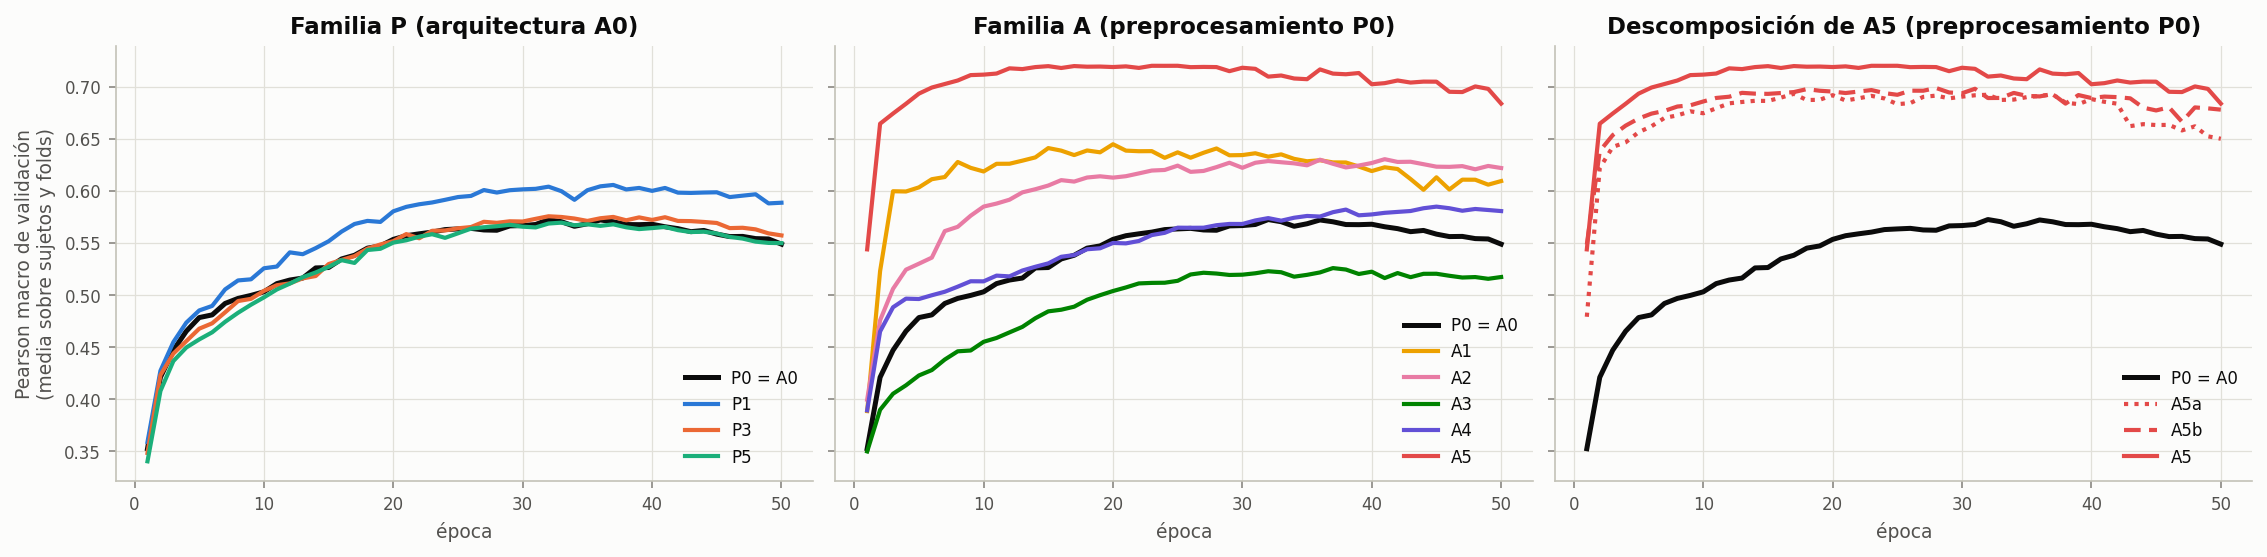
\includegraphics[width=\linewidth,height=0.44\textheight,keepaspectratio]{imgs/training_curves.png}
      \figcap{A.15}{Curvas de validaci\'on de \texttt{A5} donde el \'optimo en \texttt{S1} se alcanza antes de la \'epoca 50. \textbf{Fuente:} Obtenida del repositorio GitHub \cite{rodas_valencia_tpe_ecog}.}
      \vspace{1mm}
      \hfill\hyperlink{anexo:indice_extra}{\beamerbutton{Volver al \'Indice Extra}}
    \end{column}
  \end{columns}
\end{frame}

% --- ANEXO A16: MATEMÁTICA DE TPE, DESCOMPOSICIÓN DE +0.0672 Y VERIFICACIÓN ---
\begin{frame}{Anexo A16: Matem\'atica TPE ($\ell(\lambda)/g(\lambda)$), Descomposici\'on de $+0.0672$ y 60 Folds}{Pregunta del jurado: ?`Cu\'anto mejor\'o realmente TPE durante la b\'usqueda y cu\'anto beneficio persisti\'o al cambiar las semillas?}
  \label{anexo:tpe_diagnostico}
  \begin{columns}[c,onlytextwidth]
    \begin{column}{0.49\textwidth}
      \centering
      \resizebox{\linewidth}{!}{%
        \renewcommand{\arraystretch}{1.16}
        \begin{tabular}{>{\bfseries}l c c c c}
          \toprule
          \rowcolor{ipnDark}
          \textcolor{white}{Transici\'on / Etapa en CV} & \textcolor{white}{\texttt{S1}} & \textcolor{white}{\texttt{S2}} & \textcolor{white}{\texttt{S3}} & \textcolor{white}{Media CV} \\
          \midrule
          1. \texttt{A5} \'epoca 50 fija & $0.6038$ & $0.6216$ & $0.8258$ & $0.6837$ \\
          \rowcolor{rowLight}
          2. \texttt{A5} con checkpoint ($\Delta=+0.0493$) & $0.7103$ & $0.6466$ & $0.8422$ & $0.7330$ \\
          3. Mejor trial TPE ($\Delta=+0.0179$) & $0.7117$ & $0.6879$ & $0.8532$ & $0.7509$ \\
          \rowcolor{rowHighlight}
          4. \texttt{A5} TPE verificado ($\Delta=+0.0041$) & $0.6928$ & $\mathbf{0.6785}$ & $0.8402$ & $\mathbf{0.7372}$ \\
          \texttt{A5b} TPE verificado (60 runs) & $0.6682$ & $0.6540$ & $0.8114$ & $0.7112$ \\
          \bottomrule
        \end{tabular}%
      }
      \fuente{Creaci\'on propia, obtenida del repositorio GitHub \cite{rodas_valencia_tpe_ecog}.}

      \vspace{1.5mm}
      \begin{block}{Diagn\'ostico Estad\'istico del Aporte de TPE}
        \tiny
        \begin{itemize}\setlength{\itemsep}{1.5pt}
          \item \textbf{B\'usqueda ($+0.0179$):} Sujeta al optimismo de elegir el m\'aximo de 32 trials.
          \item \textbf{Verificaci\'on (2 semillas nuevas $\times$ 5 folds):} Ganancia global de $+0.0041$, pero mejora s\'olida y real en \textbf{\texttt{S2} ($\mathbf{+0.0319}$)}. Adem\'as, \texttt{A5} supera a \texttt{A5b} por $\mathbf{+0.0260}$ en los 3 sujetos.
        \end{itemize}
      \end{block}
    \end{column}

    \begin{column}{0.48\textwidth}
      \centering
      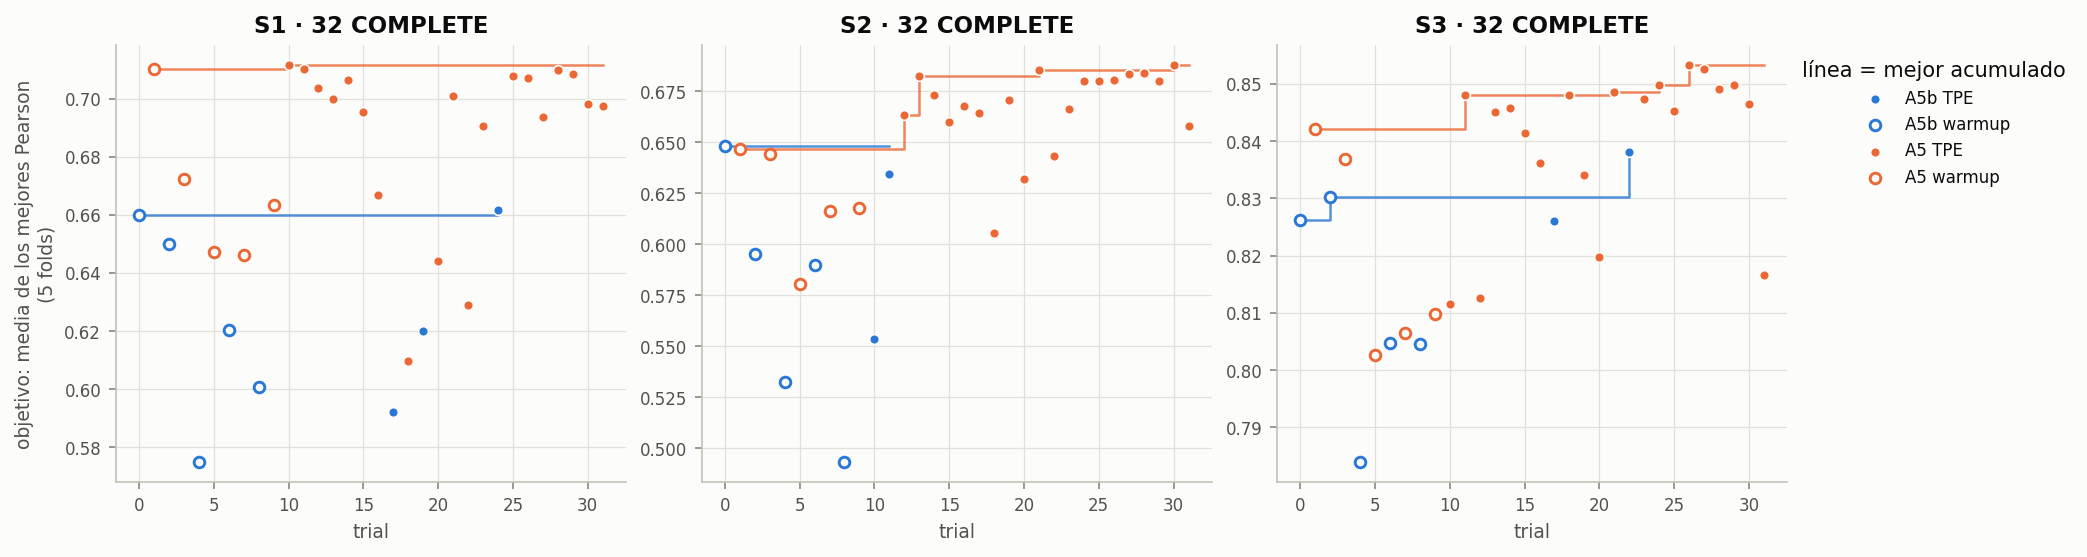
\includegraphics[width=0.48\linewidth,height=0.36\textheight,keepaspectratio]{imgs/optimization_history.png}\hfill
      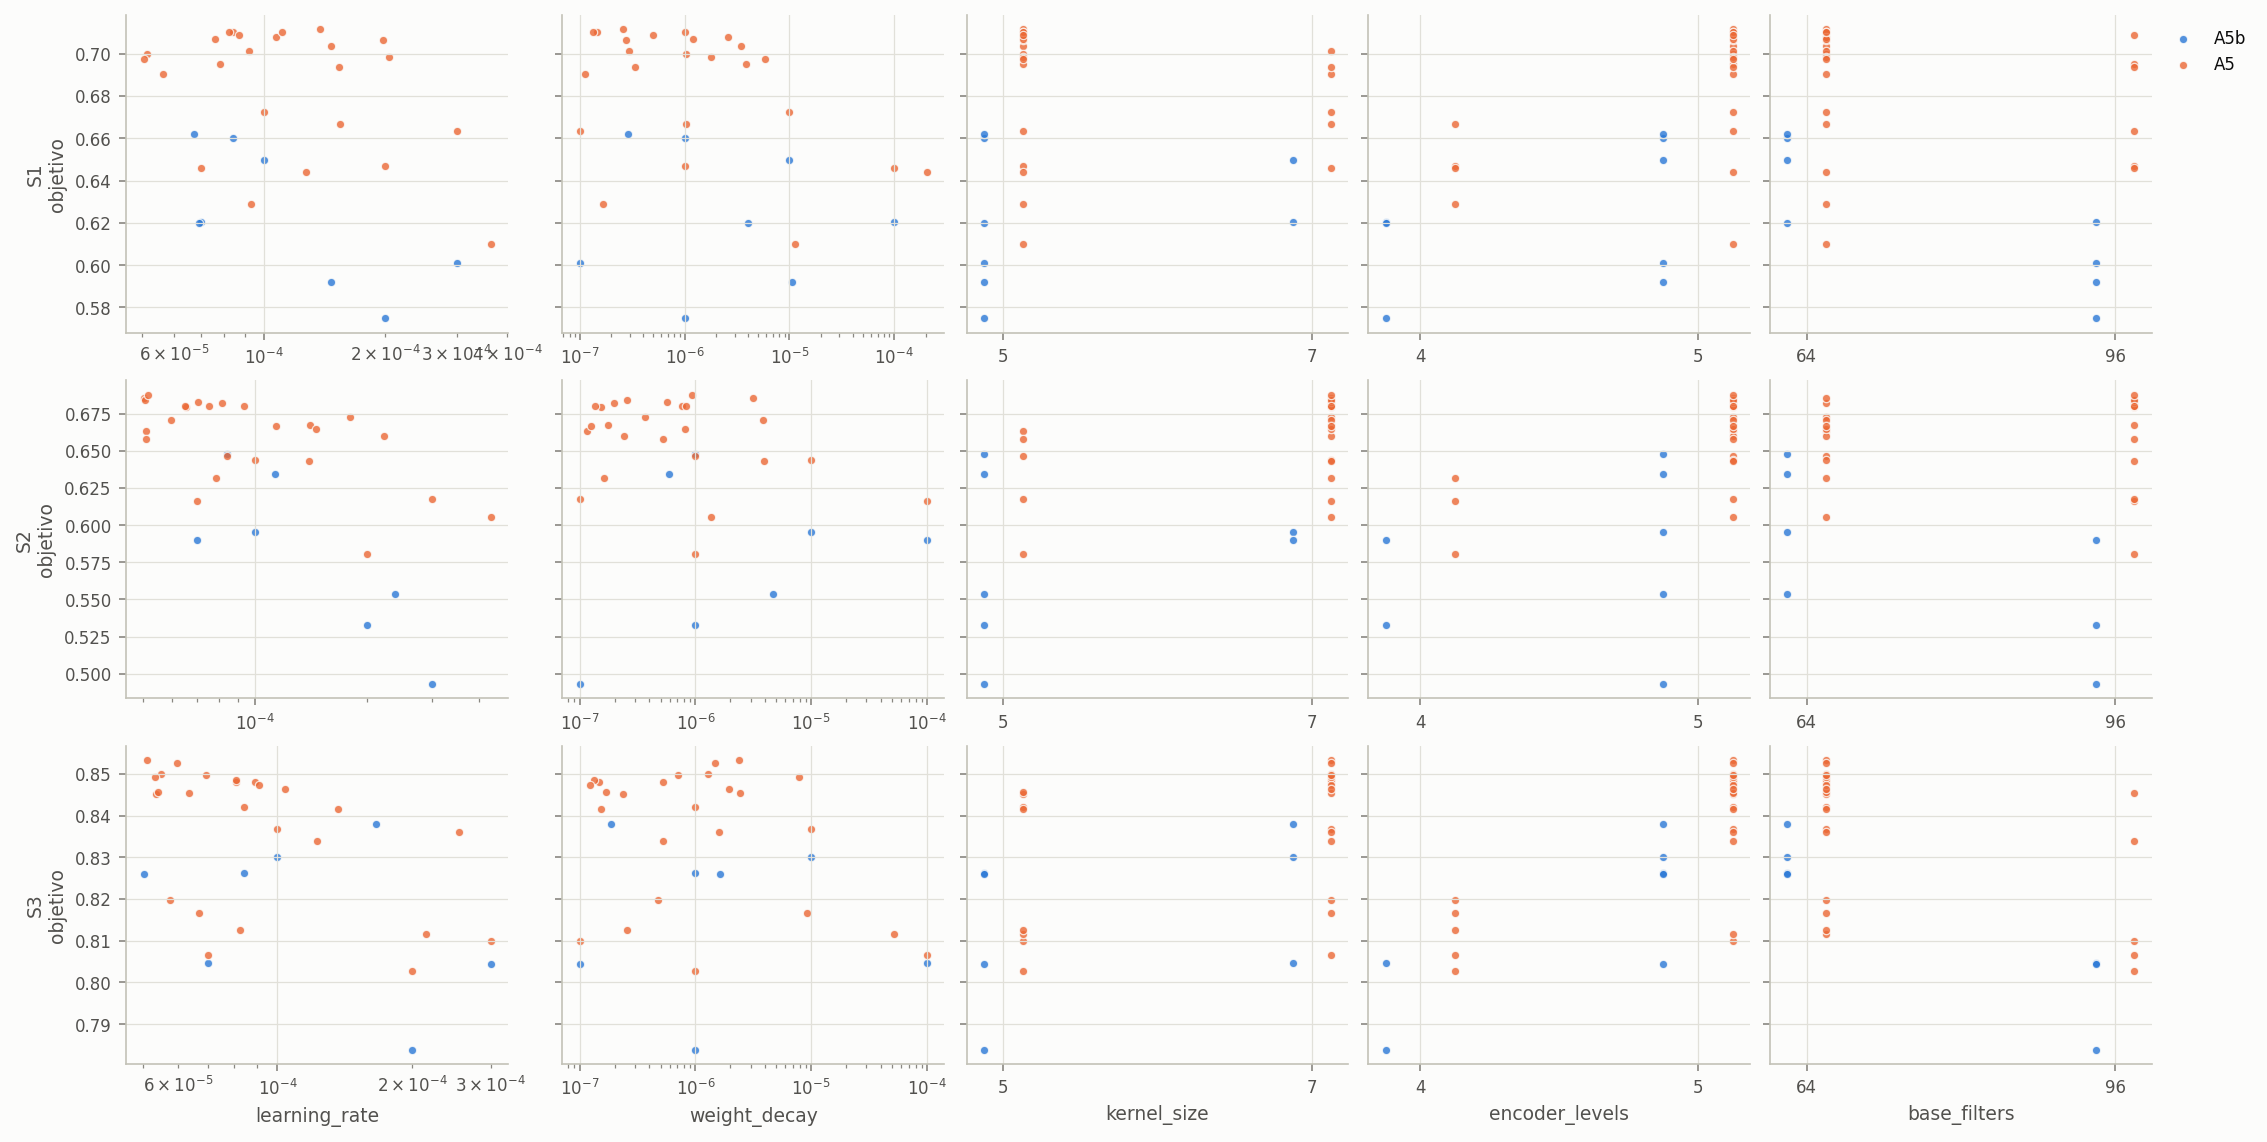
\includegraphics[width=0.48\linewidth,height=0.36\textheight,keepaspectratio]{imgs/params_vs_objective.png}
      \figcap{A.16}{Historial de los 96 trials TPE y relaci\'on par\'ametros vs.\ objetivo. \textbf{Fuente:} Obtenida del repositorio GitHub \cite{rodas_valencia_tpe_ecog}.}
      \vspace{1mm}
      \hfill\hyperlink{anexo:indice_extra}{\beamerbutton{Volver al \'Indice Extra}}
    \end{column}
  \end{columns}
\end{frame}

% --- ANEXO A17: COMPARACIÓN DE PROTOCOLOS DE TEST Y BRECHA CV VS TEST ---
\begin{frame}{Anexo A17: Protocolos de Test ($0.6333$ vs.\ $0.6669$) y Brecha CV vs.\ Test}{Pregunta del jurado: ?`Por qu\'e existe un primer test de $0.6333$ y un segundo de $0.6669$, y por qu\'e difieren del $0.7372$ de CV?}
  \label{anexo:protocolos_test_brecha}
  \centering
  \resizebox{\textwidth}{!}{%
    \renewcommand{\arraystretch}{1.18}
    \begin{tabular}{>{\bfseries}l l c c c c c c}
      \toprule
      \rowcolor{ipnDark}
      \textcolor{white}{Protocolo de Test} & \textcolor{white}{Esquema de entrenamiento final (3 semillas/sujeto)} & \textcolor{white}{\texttt{S1}} & \textcolor{white}{\texttt{S2}} & \textcolor{white}{\texttt{S3}} & \textcolor{white}{Media $r$} & \textcolor{white}{$\operatorname{CCC}$} & \textcolor{white}{$\operatorname{MSE}$} \\
      \midrule
      \texttt{b1b4\_es\_b5} (Inicial) & Entrena en \texttt{B1--B4} + \textit{Early Stopping} monitoreando \texttt{B5} & $0.6087$ & $0.5226$ & $0.7685$ & $0.6333$ & $0.5412$ & $0.6962$ \\
      \rowcolor{rowHighlight}
      \texttt{b1b5\_fixed} (Posterior) & Entrena en \texttt{B1--B5} ($100\%$) + \'epocas fijas ($21, 32, 28$) & $\mathbf{0.6723}$ & $\mathbf{0.5490}$ & $\mathbf{0.7796}$ & $\mathbf{0.6669}$ & $\mathbf{0.5759}$ & $\mathbf{0.6257}$ \\
      \midrule
      \rowcolor{rowLight}
      Diferencia ($\Delta$) & Mejora consistente en $\mathbf{9/9}$ pares sujeto-semilla & $+0.0635$ & $+0.0264$ & $+0.0111$ & $\mathbf{+0.0337}$ & $+0.0347$ & $-0.0705$ \\
      \bottomrule
    \end{tabular}%
  }
  \fuente{Creaci\'on propia, obtenida del repositorio GitHub \cite{rodas_valencia_tpe_ecog}.}

  \vspace{1.5mm}
  \begin{block}{Interpretaci\'on Prudente y Explicaci\'on de la Diferencia entre CV ($0.7372$) y Test ($0.6669$)}
    \scriptsize
    \begin{itemize}\setlength{\itemsep}{2.5pt}
      \item \textbf{Por qu\'e se reportan ambos protocolos (\texttt{tpe\_test\_protocols.csv}):} El salto de $+0.0337$ refleja el cambio de protocolo completo (incorporar \texttt{B5} al entrenamiento y fijar \'epocas de CV); como \texttt{b1b5\_fixed} se formul\'o tras observar $0.6333$, se reporta transparentemente como resultado final exploratorio.
      \item \textbf{Por qu\'e $0.7372$ (CV) vs.\ $0.6669$ (Test) no es una ``ca\'ida de entrenamiento'':} Son mediciones sobre particiones distintas: la CV promedia $5$ bloques internos de desarrollo ($320\text{ s}$), mientras que el Test eval\'ua un segmento temporal futuro e independiente ($200\text{ s}$) sujeto a deriva no estacionaria de la se\~nal ECoG \cite{rodas_valencia_tpe_ecog}. \hfill\hyperlink{anexo:indice_extra}{\beamerbutton{Volver al \'Indice Extra}}
    \end{itemize}
  \end{block}
\end{frame}

% --- ANEXO A18: COMPARACIÓN CELDA A CELDA A5 VS DTCNET ---
\begin{frame}{Anexo A18: Comparaci\'on Celda a Celda por Dedo y Sujeto: \texttt{A5} vs.\ \textit{DTCNet} (2025)}{Pregunta del jurado: ?`C\'omo se comporta nuestro modelo 1D \texttt{A5} frente a \textit{DTCNet} (3D) en cada dedo individual?}
  \label{anexo:comparacion_dtcnet_dedos}
  \begin{columns}[c,onlytextwidth]
    \begin{column}{0.55\textwidth}
      \centering
      \resizebox{\linewidth}{!}{%
        \renewcommand{\arraystretch}{1.16}
        \begin{tabular}{>{\bfseries}l c c c c c c}
          \toprule
          \rowcolor{ipnDark}
          \textcolor{white}{Sujeto (Modelo)} & \textcolor{white}{Pulgar} & \textcolor{white}{\'Indice} & \textcolor{white}{Medio} & \textcolor{white}{Anular} & \textcolor{white}{Me\~nique} & \textcolor{white}{Media} \\
          \midrule
          \texttt{S1} --- \texttt{A5} vs.\ \textit{DTCNet} & $0.6135 / 0.69$ & $\mathbf{0.7909} / 0.76$ & $0.6320 / 0.76$ & $0.7188 / 0.74$ & $\mathbf{0.6061} / 0.60$ & $0.6723 / 0.71$ \\
          \rowcolor{rowLight}
          \texttt{S2} --- \texttt{A5} vs.\ \textit{DTCNet} & $\mathbf{0.6241} / 0.62$ & $0.6087 / 0.67$ & $0.4107 / 0.52$ & $\mathbf{0.6280} / 0.56$ & $0.4733 / 0.58$ & $0.5490 / 0.59$ \\
          \texttt{S3} --- \texttt{A5} vs.\ \textit{DTCNet} & $\mathbf{0.8367} / 0.82$ & $\mathbf{0.7487} / 0.73$ & $0.6798 / 0.72$ & $\mathbf{0.8137} / 0.81$ & $\mathbf{0.8190} / 0.77$ & $\mathbf{0.7796} / 0.77$ \\
          \midrule
          \rowcolor{rowHighlight}
          Media \texttt{A5} vs.\ \textit{DTCNet} & $0.6914 / 0.70$ & $0.7161 / 0.72$ & $0.5742 / 0.67$ & $\mathbf{0.7202 / 0.70}$ & $0.6328 / 0.65$ & $0.6669 / 0.69$ \\
          Diferencia ($\Delta r$) & $-0.0086$ & $-0.0039$ & $\mathbf{-0.0958}$ & $\mathbf{+0.0202}$ & $-0.0172$ & $-0.0231$ \\
          \bottomrule
        \end{tabular}%
      }
      \fuente{Creaci\'on propia a partir de \cite{wang2025dtcnet} y el repositorio GitHub \cite{rodas_valencia_tpe_ecog}.}

      \vspace{1.5mm}
      \begin{block}{Hallazgo Clave de la Comparaci\'on en las 15 Celdas}
        \tiny
        \texttt{A5} \textbf{supera a \textit{DTCNet} \cite{wang2025dtcnet} en 8 de los 15 pares sujeto-dedo}, en la media del \textbf{Sujeto 3 ($0.7796$ vs.\ $0.77$)} y en el promedio global del \textbf{dedo Anular ($+0.0202$)}. M\'as del $\mathbf{83\%}$ de la brecha global proviene exclusivamente del dedo Medio ($-0.0958$).
      \end{block}
    \end{column}

    \begin{column}{0.42\textwidth}
      \centering
      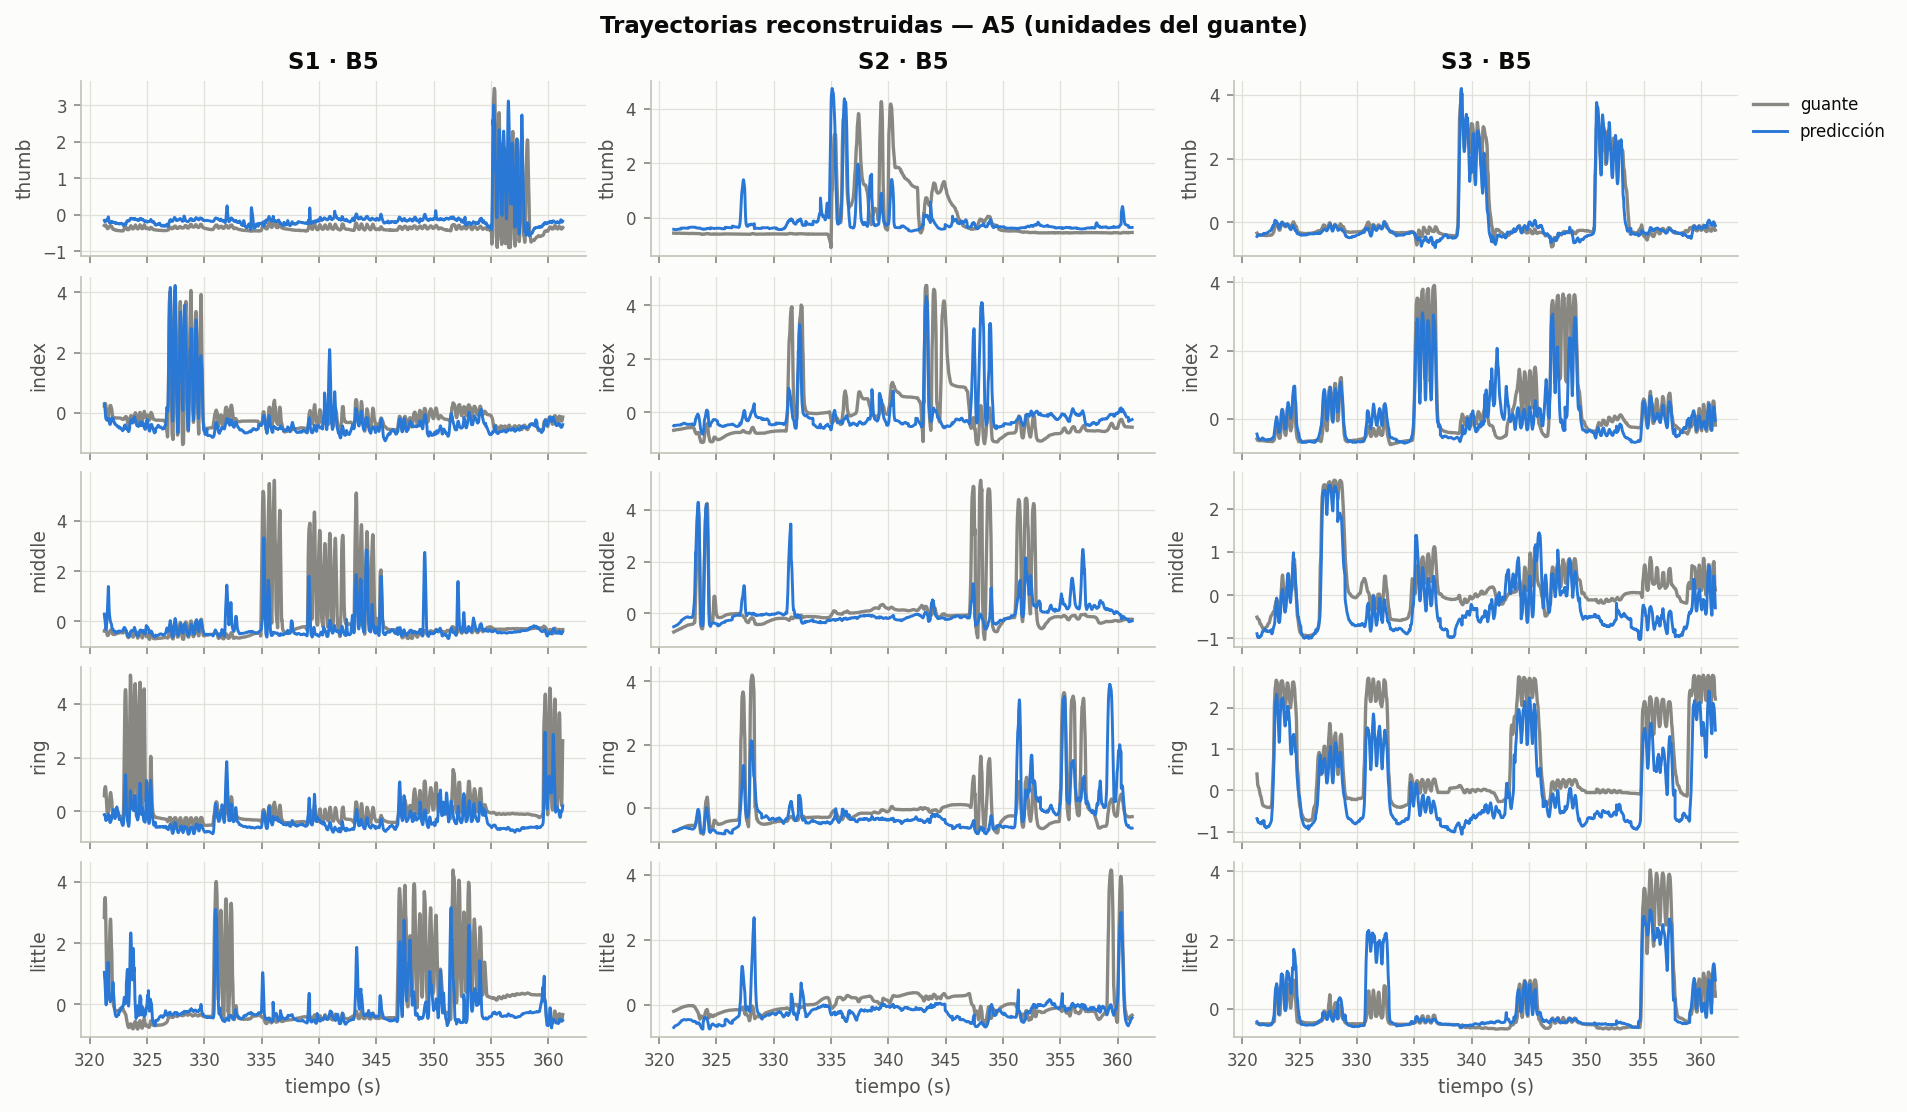
\includegraphics[width=\linewidth,height=0.42\textheight,keepaspectratio]{imgs/example_predictions_A5_B5.png}
      \figcap{A.17}{Reconstrucci\'on de \texttt{A5} en \texttt{B5}. \textbf{Fuente:} Obtenida de GitHub \cite{rodas_valencia_tpe_ecog}.}
      \vspace{1mm}
      \hfill\hyperlink{anexo:indice_extra}{\beamerbutton{Volver al \'Indice Extra}}
    \end{column}
  \end{columns}
\end{frame}

% --- ANEXO A19: MATRIZ DE TRAZABILIDAD COMPUTACIONAL ---
\begin{frame}{Anexo A19: Matriz Completa de Trazabilidad Computacional (Archivos CSV)}{Pregunta del jurado: ?`De qu\'e archivo exacto proviene cada cifra reportada en el documento y en las diapositivas?}
  \label{anexo:trazabilidad_csv}
  \begin{columns}[T,onlytextwidth]
    \begin{column}{0.60\textwidth}
      \centering
      \tiny
      \renewcommand{\arraystretch}{0.95}
      \begin{tabularx}{\linewidth}{>{\ttfamily\color{ipnDark}}l >{\raggedright\arraybackslash}X}
        \toprule
        \rowcolor{ipnDark}
        \textcolor{white}{\normalfont\textbf{Archivo CSV de Respaldo}} & \textcolor{white}{\textbf{Contenido Experimental Auditado (Secci\'on 9)}} \\
        \midrule
        results\_subjects.csv & Medias por sujeto en ablaciones (\'epoca 50, \texttt{A0--A5}, \texttt{P0--P5}). \\
        \rowcolor{rowLight}
        results\_all.csv & Resultados por pliegue, sujeto y dedo en ablaciones. \\
        history\_A5b / history\_A5.csv & Curvas train/val \'epoca por \'epoca ($1\text{--}50$). \\
        \rowcolor{rowLight}
        paired\_deltas[\_summary].csv & Deltas apareados por pliegue ($\texttt{A0}\to\texttt{A5}$, $14/15$ $+$). \\
        summary/ablation\_retrospective.csv & Simulaci\'on retrospectiva de checkpoint ($0.6837 \to 0.7330$). \\
        \rowcolor{rowLight}
        summary/tpe\_trials / tpe\_folds.csv & Historial de los $96$ trials TPE y m\'etricas por fold/par\'ametros. \\
        summary/tpe\_comparison.csv & Descomposici\'on entre \'epoca 50, checkpoint y TPE. \\
        \rowcolor{rowLight}
        summary/tpe\_verification.csv & Verificaci\'on multi-semilla ($60$ runs: \texttt{A5} $0.7372$ vs.\ \texttt{A5b} $0.7112$). \\
        summary/tpe\_selected\_models.csv & Hiperpar\'ametros ganadores y mediana de \'epoca ($21, 32, 28$). \\
        \rowcolor{rowLight}
        summary/tpe\_verification\_paired*.csv & Contrastes apareados en verificaci\'on (\texttt{S2} $+0.0319$). \\
        summary/tpe\_test[\_summary].csv & Test Oficial por semilla, sujeto y dedo ($r=0.6669$). \\
        \rowcolor{rowLight}
        summary/tpe\_test\_protocols.csv & Comparaci\'on \texttt{b1b4\_es\_b5} ($0.6333$) vs.\ \texttt{b1b5\_fixed} ($0.6669$). \\
        \bottomrule
      \end{tabularx}
      \fuente{Creaci\'on propia a partir de los registros del repositorio GitHub \cite{rodas_valencia_tpe_ecog}.}
    \end{column}

    \begin{column}{0.38\textwidth}
      \begin{block}{6 Reglas Oficiales de C\'alculo}
        \tiny
        \begin{enumerate}\setlength{\itemsep}{1pt}
          \item \textbf{Precisi\'on completa:} Toda media se calcula en coma flotante antes de redondear a $4$ decimales.
          \item \textbf{Jerarqu\'ia:} $5\text{ dedos} \to \text{pliegue/semilla} \to \text{sujeto} \to \text{media global}$.
          \item \textbf{Trayectoria completa:} Pearson medido tras \textit{overlap-add}, nunca en ventanas sueltas.
          \item \textbf{Deltas apareados:} $\Delta r$ calculado sin redondear ($\pm 0.0001$).
          \item \textbf{Verificaci\'on limpia:} Excluye la semilla de b\'usqueda.
          \item \textbf{Cero edici\'on manual:} Exportaci\'on directa desde scripts.
        \end{enumerate}
      \end{block}
      \hfill\hyperlink{anexo:indice_extra}{\beamerbutton{Volver al \'Indice Extra}}
    \end{column}
  \end{columns}
\end{frame}

% --- ANEXO A20: GOBERNANZA DE DATOS Y PODA ESTRUCTURADA ---
\begin{frame}{Anexo A20: Gobernanza de Datos Biom\'edicos y Poda Estructurada (Trabajo Futuro)}{Pregunta del jurado: ?`C\'omo se cumple el manejo de datos sensibles y c\'omo reducir el tama\~no ($9.35\text{--}28.03\text{ M}$) para un sistema embebido?}
  \label{anexo:poda_y_privacidad}
  \begin{columns}[T,onlytextwidth]
    \begin{column}{0.45\textwidth}
      \begin{block}{1. Gobernanza y Anonimizaci\'on de Datos Cl\'inicos}
        \scriptsize
        \begin{itemize}\setlength{\itemsep}{3pt}
          \item \textbf{Benchmark p\'ublico internacional:} Se utiliz\'o exclusivamente el corpus \textit{BCI Competition IV --- Dataset 4} \cite{miller2008prediction}, recolectado en el \textit{Harborview Medical Center} (University of Washington).
          \item \textbf{Anonimizaci\'on de origen:} Los registros ECoG se distribuyen desprovistos de metadatos personales (\texttt{sub1}, \texttt{sub2}, \texttt{sub3}), cumpliendo con los protocolos internacionales de privacidad biom\'edica.
        \end{itemize}
      \end{block}
    \end{column}

    \begin{column}{0.52\textwidth}
      \begin{block}{2. Formulaci\'on Proyectiva de Poda Estructurada (Trabajo Futuro)}
        \scriptsize
        Para comprimir las capas profundas ($4f$ y $8f$) de \texttt{A5} hacia hardware neuroprot\'esico de bajo consumo, se plantea como \textbf{propuesta matem\'atica de trabajo futuro} evaluar la importancia de cada filtro $o \in \{1,\dots,C_{\text{out}}\}$ mediante la norma $\ell_1$ y el factor de escala $\gamma_o$ de \texttt{LayerNorm}:
        \[
          \mathcal{I}_{\ell_1}(o) = \sum_{c=1}^{C_{\text{in}}}\sum_{m=1}^{k} |W_{o,c,m}|, \qquad \mathcal{I}_{\text{LN}}(o) = |\gamma_o|\cdot \|\mathbf{W}_{o,:,:}\|_2
        \]
        eliminando f\'isicamente los canales con menor contribuci\'on antes de reentrenar (\textit{fine-tuning}) o destilar hacia un modelo estudiante ligero \cite{rodas_valencia_tpe_ecog}.
      \end{block}
      \vspace{1mm}
      \hfill\hyperlink{anexo:indice_extra}{\beamerbutton{Volver al \'Indice Extra}}
    \end{column}
  \end{columns}
\end{frame}

\annexslidefalse


\end{document}
